\documentclass[12pt]{article}
% AAU theme adapted from the preamble supplied by the project team.
\usepackage[a4paper,margin=1in]{geometry}
\usepackage{lmodern}
\usepackage[T1]{fontenc}
\usepackage{microtype}
\usepackage{graphicx}
\usepackage{float}
\usepackage{amsmath}
\usepackage[table]{xcolor}
\usepackage{titlesec}
\usepackage{fancyhdr}
\usepackage[most]{tcolorbox}
\PassOptionsToPackage{obeyspaces}{url}
\usepackage[hidelinks]{hyperref}
\usepackage{array}
\usepackage{tabularx}
\usepackage{enumitem}
\usepackage{booktabs}
% Vector UML artwork and multipage test tables.
\usepackage{longtable}
\usepackage{pdflscape}
\definecolor{aauRed}{RGB}{164,22,35}
\definecolor{aauGreen}{RGB}{0,122,88}
\definecolor{darkGray}{RGB}{60,60,60}
\definecolor{softGray}{RGB}{245,245,245}
\pagestyle{fancy}\fancyhf{}\fancyfoot[C]{\thepage}
\renewcommand{\headrulewidth}{0pt}\renewcommand{\footrulewidth}{0pt}
\titleformat{\section}{\normalfont\Large\bfseries\color{aauRed}}{\thesection}{0.6em}{}[{\color{aauRed!65}\titlerule[1.1pt]}]
\titlespacing*{\section}{0pt}{12pt}{8pt}
\titleformat{\subsection}{\normalfont\normalsize\bfseries\color{aauRed!85!black}}{\thesubsection}{0.6em}{}
\titlespacing*{\subsection}{0pt}{10pt}{4pt}
\newtcolorbox{objectivebox}{enhanced,colback=aauRed!5,colframe=aauRed!80!black,boxrule=0.3mm,arc=1mm,left=10pt,right=10pt,top=6pt,bottom=6pt,borderline west={2.5pt}{0pt}{aauRed}}
% Each short use/test case stays on one page, including its heading.
\newtcolorbox{contentbox}[1][]{enhanced,colback=softGray,colframe=black!35,boxrule=0.25mm,arc=2mm,left=9pt,right=9pt,top=7pt,bottom=7pt,before skip=9pt,after skip=9pt,title={\textbf{#1}},fonttitle=\bfseries,coltitle=darkGray,colbacktitle=black!8}
\newcommand{\blankline}{\rule{\linewidth}{0.35pt}}
\newcommand{\insertfigure}[3]{\begin{figure}[H]\centering\fbox{\parbox[c][#2][c]{0.88\textwidth}{\centering\textcolor{black!50}{\Large #1}}}\caption{#3}\end{figure}}
\newcommand{\screen}[3][0.98]{\begin{figure}[H]\centering\includegraphics[width=#1\linewidth]{../assets/#2}\caption{#3}\end{figure}}
% Give wide UML models a dedicated landscape page with readable labels.
\newenvironment{umlpage}{%
\newgeometry{margin=0.65in}\begin{landscape}\pagestyle{empty}%
\AddToHook{shipout/foreground}[arena/umlfooter]{%
\begin{tikzpicture}[remember picture,overlay]
\node[rotate=90,anchor=south,inner sep=0pt] at ([xshift=-23pt]current page.east)
{\normalfont\normalsize\thepage};
\end{tikzpicture}}%
}{\end{landscape}\RemoveFromHook{shipout/foreground}[arena/umlfooter]\pagestyle{fancy}\restoregeometry}
\newcommand{\umlfigure}[2]{\begin{figure}[H]\centering
\includegraphics[width=\linewidth,height=13cm,keepaspectratio]{../assets/uml/#1.pdf}
\caption{#2}\end{figure}}
\providecommand{\reportdate}{10 November 2026}
% Two intentionally sized figures fit together with a heading on an A4 page.
\newcommand{\screenpair}[5][0.30]{%
\begin{figure}[H]\centering
\includegraphics[width=0.96\linewidth,height=#1\textheight,keepaspectratio]{../assets/#2}\caption{#3}
\vspace{8pt}
\includegraphics[width=0.96\linewidth,height=#1\textheight,keepaspectratio]{../assets/#4}\caption{#5}
\end{figure}}
\setlength{\parindent}{0pt}\setlength{\parskip}{5pt}
\setlist[itemize]{leftmargin=1.5em,itemsep=2pt,topsep=3pt}
\setlist[enumerate]{leftmargin=1.7em,itemsep=3pt,topsep=4pt}
\setlength{\emergencystretch}{2em}
\widowpenalty=10000\clubpenalty=10000\displaywidowpenalty=10000
\brokenpenalty=10000
\raggedbottom
\renewcommand{\arraystretch}{1.16}
\setlength{\abovecaptionskip}{7pt}
\setlength{\belowcaptionskip}{4pt}
\setlength{\intextsep}{12pt plus 2pt minus 2pt}
\newcolumntype{Y}{>{\raggedright\arraybackslash}X}
\BeforeBeginEnvironment{tabularx}{\par\noindent}
\AfterEndEnvironment{tabularx}{\par}
\newcommand{\code}[1]{{\small\expandafter\nolinkurl\expandafter{\detokenize{#1}}}}
\newcommand{\command}[1]{\mbox{\small\ttfamily\detokenize{#1}}}
\newcommand{\projecttitle}[2]{%
\hypersetup{pageanchor=false}\begin{titlepage}\centering\vspace*{-0.45cm}
\noindent\begin{minipage}[c]{0.66\textwidth}\raggedright
{\Large\bfseries Al Ain University (AAU)\par}
\end{minipage}\hfill
\begin{minipage}[c]{0.28\textwidth}\raggedleft
% The supplied PNG is unchanged; trim removes only its transparent margins.
\includegraphics[width=3.1cm,trim=1731bp 871bp 1735bp 878bp,clip]{../../aau.png}
\end{minipage}\par
\vspace{0.45cm}
{\scshape\large Object Oriented Analysis and Design\par}
\vspace{0.10cm}
{\normalsize System Analysis \& Design\par}
\vspace{0.10cm}
{\small Course codes: 0103430 \;|\; 0102331\par}
\vspace{0.3cm}\noindent\rule{\linewidth}{0.5mm}\par\vspace{0.3cm}
{\huge\bfseries Arena\par}
\vspace{0.18cm}{\Large\color{aauRed}#1\par}
\vspace{0.15cm}{\normalsize\color{darkGray}#2\par}
\vspace{0.12cm}{\color{aauRed}\rule{\linewidth}{1.2pt}\par}
\vspace{0.35cm}{\normalsize\bfseries Prepared by\par}\vspace{0.15cm}
\begin{tabular}{@{}lr@{}}\textbf{Name}&\textbf{Student ID}\\\midrule
Khaled Alkhawaldeh&202410091\\Abdulrahman Alnaqbi&202340042\\Yousif Alhammadi&202310707\\Ahmed Alsamma&202320192\end{tabular}\par
\vspace{0.22cm}{\color{aauRed!55}\rule{0.6\textwidth}{1.2pt}\par}
\vspace{0.15cm}{\normalsize\textbf{Section:} 61D\par}
\vspace{0.15cm}{\normalsize\textbf{Submitted to:} Dr. Yazeed Ghadi\par}
\vspace{0.3cm}
\begin{tcolorbox}[colback=gray!5,colframe=black!70,title=\textbf{Project Summary},fonttitle=\bfseries,width=0.95\textwidth,boxrule=0.4mm,arc=3mm,left=7pt,right=7pt,top=4pt,bottom=4pt]
A Java desktop workspace for organizing campus competitions, coordinating teams, collecting submissions, evaluating work, and publishing results. Project, programming, and quiz scoring are separated from score-ranking, knockout, and league progression through object-oriented strategies. The application is developed for Al Ain University in the United Arab Emirates.
\end{tcolorbox}
\vfill{\normalsize Fall, 2026--2027\par}{\small Version 2.0 \;|\; \reportdate\par}
\end{titlepage}\pagenumbering{roman}\hypersetup{pageanchor=true}\tableofcontents\clearpage\pagenumbering{arabic}}


\geometry{a4paper,margin=0.85in}
\hypersetup{pdftitle={Understanding Arena: From Requirements to Running Code},pdfauthor={Arena project learning guide}}
\newcommand{\topic}[1]{\needroom{9\baselineskip}\section{#1}}
\newcommand{\needroom}[1]{\par\begingroup\dimen0=\pagegoal\advance\dimen0 by -\pagetotal\ifdim\dimen0<#1\newpage\fi\endgroup}
\newcommand{\method}[2]{\par\textcolor{aauGreen}{\code{#1}}. #2\par}
\begin{document}
\hypersetup{pageanchor=false}
\begin{titlepage}
\centering
\includegraphics[width=3.3cm,trim=1731bp 871bp 1735bp 878bp,clip]{../aau.png}\par
\vspace{1cm}
{\large Al Ain University\par}
\vspace{0.5cm}
{\huge\bfseries Understanding Arena\par}
\vspace{0.4cm}
{\Large From requirements to running Java code\par}
\vspace{0.3cm}
{\color{aauRed}\rule{\linewidth}{1.2pt}}
\vspace{0.4cm}
{\large Arena\par}
\vspace{0.7cm}
\begin{objectivebox}
This guide explains the actual repository for a reader who already knows basic Java. It connects the assignment, reports, UML, domain model, application service, interface, persistence, tests, and presentation. It also identifies simplifications and limitations so you can explain the project accurately.
\end{objectivebox}
\vspace{0.5cm}
{\normalsize Object Oriented Analysis and Design / System Analysis \& Design\par}
{\normalsize 0103430 / 0102331\quad Section 61D\par}
{\normalsize Instructor: Dr. Yazeed Ghadi\par}
\vspace{0.6cm}
Khaled Alkhawaldeh\quad 202410091\par
Abdulrahman Alnaqbi\quad 202340042\par
Yousif Alhammadi\quad 202310707\par
Ahmed Alsamma\quad 202320192\par
\vfill
Personal study companion, not an additional assessed report\par
Code reviewed: 10 November 2026\par
File locations updated: 10 November 2026\par
\small Prepared with AI assistance; individual development contributions are not inferred.
\end{titlepage}
\pagenumbering{roman}
\hypersetup{pageanchor=true}
\tableofcontents
\clearpage\pagenumbering{arabic}

\topic{The whole project in one connected explanation}
Arena organizes campus competitions from the moment an organizer defines an event until its results are published and archived. A student joins a team; that team's captain registers it. A project or programming team submits work. Assigned judges enter assessments. A knockout judge instead decides matches. The organizer advances the competition only when the work required for its current stage is complete.

The central design problem is \textbf{variation}. A project wins through quality scores, a programming entry through solved problems and penalties, and a knockout entrant through elimination matches. Those are different rules and different workflows. The system reuses accounts, teams, registrations, publication, and storage while making the differences explicit.

\begin{contentbox}[Your first explanation to the professor]
``Our system manages the complete competition lifecycle. We model shared concepts such as users, teams, and registrations, then separate format-specific validation and scoring through a CompetitionRules and TournamentRules interfaces. ArenaService enforces permissions and workflow guards. Swing presents those operations, and Repository saves the data locally. We demonstrate project, programming and quiz scoring, knockout progression and league standings because they require different policies.''
\end{contentbox}

\subsection{What exists, and what each part contributes}
\begin{tabularx}{\linewidth}{lY}\toprule Part & Purpose\\\midrule
Assignment outlines & What academic sections and deliverables were requested.\\
Analysis report & What problem is being solved, who uses it, and what behavior is required.\\
Design report & How responsibilities, objects, dependencies, and policies are organized.\\
Java application & Executable implementation of those decisions.\\
Browser prototype & A separate interactive demonstration of appearance and intended flows.\\
Tests and evidence & Repeatable checks, plus stored results of a particular execution.\\
Implementation report & What was built, why choices were made, limits, and how to run it.\\
Presentation & A selective explanation and live demonstration of the strongest OOAD ideas.\\\bottomrule
\end{tabularx}

The Java app is a local desktop program. Swing creates native Java windows. There is no web backend, remote API, SQL server, or connection from the browser prototype to the Java app. Different people use different accounts sequentially in one application process.

\subsection{Follow one action across the architecture}
\begin{enumerate}
\item A captain clicks Register my team in the Swing interface.
\item AppDialogs collects a team choice and calls \code{service.register(competitionId, teamId)}.
\item ArenaService gets the authenticated identity from its own session. It checks captain ownership, phase, deadline, capacity, roster size, duplicate registration, and overlapping members.
\item The service creates a Registration record inside its \code{change} helper. This also creates an audit entry.
\item Repository saves the complete State. If saving fails, the service restores its previous in-memory snapshot.
\item The interface reloads the competition view. The team appears only after the operation succeeds.
\end{enumerate}
This is the same idea shown by the registration sequence diagram. A button click is merely the beginning of the use case; the important behavior is the controlled state change behind it.

\topic{What the assignment and reports actually mean}
\subsection{The professor's requirement versus our design choices}
The supplied professor message approved the topic and explicitly asked for more than registration and scheduling, including different competition formats and variations in rules and workflows. The original text files provide report outlines. They do not prescribe a 40/35/25 rubric, a 20-minute penalty, Swing, Java serialization, or a particular package structure. Those are documented implementation decisions, not quotations from the assignment.

Analysis means deciding \emph{what the system must do}. Design means deciding \emph{how software responsibilities will realize it}. Implementation means writing executable code. Verification means checking it against its requirements. Validation asks whether it solves the intended user problem. Automated checks provide verification evidence; they do not replace a real user study.

\subsection{Read the System Analysis report}
The Introduction explains fragmented competition management, the objectives, scope, technology assumptions, and team identity. The Overview introduces users and contrasts the formats. Functional Requirements describe observable actions. Nonfunctional Requirements describe qualities and constraints. System Models show actors, interactions, flow, state, and domain relationships. UI material translates those ideas into screens. The glossary explains terms; references identify the technical material used.

\begin{longtable}{p{0.14\linewidth}p{0.78\linewidth}}\toprule Requirement & Meaning in this project\\\midrule\endhead
FR-01 & Email/password authentication and sign-out. A failed login clears the previous session.\\
FR-02 & Administrator-created accounts with unique email, assigned role, and password validation; users change their own password.\\
FR-03 & Create and edit drafts, assign judges, and advance through guarded phases. Only the owner or an administrator manages an event.\\
FR-04 & Captain-led registration and withdrawal. Reject full events, duplicate entries, oversized rosters, overlap, and late registration.\\
FR-05 & Student team creation, joining, leaving as a noncaptain, and roster locking after registration.\\
FR-06 & Registered captains submit or replace work while Active and before the deadline. Submission reads are scoped.\\
FR-07 & Assigned judges evaluate during Judging. Validate score ranges and feedback; replace only that judge's earlier review.\\
FR-08 & Protected provisional results, publication completeness, shared ranks, and CSV export.\\
FR-09 & Programming scores: solved count and penalty; one official result owner per entry.\\
FR-10 & Power-of-two knockout entries, seeded rounds, final match decisions, and champion progression.\\
FR-11 & Successful changes produce audit entries; staff can see the latest 2,000.\\\bottomrule
\end{longtable}

NFR-01 concerns responsiveness for small datasets. The under-one-second target is an unmeasured design goal. NFR-02 concerns password derivation, permissions, and constrained deserialization. NFR-03 concerns clear screens, labels, empty states, and minimum window size. NFR-04 concerns persistence, rollback, locks, and preserving corrupt files. NFR-05 concerns separation and testability. An NFR is not automatically satisfied just because it appears in a report: look for implementation and evidence, and retain stated gaps.

\subsection{Read the System Design report}
The design goals explain the intended structure. Subsystem decomposition assigns responsibilities to the UI, service, model/rules, and infrastructure. Hardware/software mapping means one JVM on one computer. Persistent data management describes how records become a file. Access control identifies who may act. Boundary conditions describe first launch, existing data, bad input, duplicate instances, and closing.

Subsystem services are groups of use cases, not separate network services. Low-level design discusses records, role composition, Strategy, and storage trade-offs. The class catalogue maps domain concepts to fields and methods. Its invariants are facts that must remain true after valid service operations: for example, a match winner must be one of its two entrants.

\subsection{Read the Implementation Report and User Guide}
The implementation section names the technologies and delivered features. Challenges explain why particular fixes were necessary. Design changes distinguish decisions made during implementation from an imaginary previously approved architecture. The testing summary points to evidence. Project status distinguishes delivered work from exclusions. Team collaboration labels individual responsibilities as proposed, not verified historical authorship. The appendix is the User Guide: setup, accounts, procedures, screenshots, and troubleshooting.

Do not say the team independently implemented a particular feature unless that contribution is confirmed. The reports disclose AI assistance. Presentation ownership is an allocation of speaking responsibilities, not proof of development authorship.

\subsection{Read the Testing and Interface reports}
The Testing Report explains strategy, setups, steps, expected outcomes, recorded outcomes, defects, and gaps. Its tables come from CSV evidence; they are not a list of tests that merely ought to exist. A test's date matters because later edits are not automatically covered by an older execution.

The Interface Mock-ups document contains monochrome skeletons, browser prototype captures, and actual Swing renders. A wireframe shows information placement. A prototype simulates interaction and visual style. A screenshot records an implemented screen. They are three different types of evidence.

\subsection{How the LaTeX documents work}
Each report now has one clearly named source in \code{reports/source}, such as \code{system-analysis.tex}. That file contains both the compilation entry point and the report text. It loads the shared AAU style before the document content. The preamble controls A4 margins, fonts, AAU red/green colors, headings, boxes, tables, page numbers, cover, and image helpers. Content uses sections, tables, formulas, captions, and input statements rather than manually positioning every word.

\code{aau.png} is the original university logo. LaTeX trims its transparent margins for display without editing the file. \code{screenpair} places two captures on a page. \code{umlfigure} embeds a vector PDF; \code{umlpage} uses landscape pages. SVG originals are editable drawings; matching PDFs are LaTeX-compatible vector assets. These are necessary illustrations, not screenshots of entire report pages. Compilation produces the final five PDFs; intermediate logs and auxiliary files belong in ignored build folders.

\topic{Actors, permissions, and the domain language}
\subsection{Roles are not the same as ownership}
The four Role values are ADMIN, ORGANIZER, JUDGE, and STUDENT. Captain is a relationship: a student's ID equals a particular team's captainId. Owner is another relationship: an organizer's ID equals a competition's organizerId. Assigned judge means the user ID belongs to a competition's judgeIds set.

A judge role alone does not authorize scoring every competition. An organizer role alone does not authorize changing another organizer's event. An administrator may manage any event and create accounts, but cannot record a judge's evaluation merely by being an administrator. The code deliberately separates management authority from judging authority.

\begin{tabularx}{\linewidth}{Ycccc}\toprule Action & Student & Judge & Organizer & Admin\\\midrule
Browse / official results & Yes & Yes & Yes & Yes\\
Create / join teams & Yes & No & No & No\\
Register / submit & Captain & No & No & No\\
Create event & No & No & Yes & Yes\\
Edit / advance event & No & No & Owner & Any\\
Evaluate / decide match & No & Assigned & No & No\\
Create accounts & No & No & No & Yes\\
Read audit & No & No & Yes & Yes\\\bottomrule\end{tabularx}

Authentication answers ``who signed in?'' Authorization answers ``may that person do this to this event now?'' A valid identity can still be rejected for wrong role, wrong ownership, wrong phase, or invalid data. Hiding a UI button improves usability; service checks enforce the boundary even when tests call methods directly.

\subsection{The objects you must keep separate}
A User is an account. A Team is a persistent group of students. A Competition is an event with rules and a phase. A Registration links one team to one event. A team can enter multiple events without being copied into multiple Team records.

A Submission is the team's current title, description, and URL for one entry. An Evaluation is one judge's assessment of an entry. Replacing a submission does not mean creating a team. Revising a review does not mean registering again. A Match pairs two team IDs in one round. A Standing is a calculated result row; it is not another stored score. Audit records a successful change.

\begin{contentbox}[Example using stable IDs]
Team Alpha has ID \code{alpha}, captain \code{student1}, and members \code{student1}, \code{student2}. A Registration can link \code{alpha} to \code{hackathon}, and another can link the same team to \code{robotics}. A judge's evaluation stores the competition ID, team ID, and judge ID. The service follows these IDs to retrieve the relevant records.
\end{contentbox}

\subsection{Type, tournament format and phase answer different questions}
CompetitionType answers what participants do: PROJECT, PROGRAMMING, QUIZ or MATCH. TournamentFormat answers how a winner emerges: score ranking, knockout or round robin. Phase answers where the event is in its lifecycle. A quiz can use points ranking, a knockout bracket or a league. Project and programming only support ranking; general matches support knockout or league. The compatibility check belongs to the model/service, so bypassing the form cannot create an unsupported combination.

\topic{Competition types, tournament formats and their complete workflows}
\subsection{The shared lifecycle}
\begin{center}\small
Draft $\rightarrow$ Registration $\rightarrow$ Active $\rightarrow$ Judging $\rightarrow$ Published $\rightarrow$ Archived
\end{center}
There is one explicit phase value per event. The owning organizer or an administrator requests each transition. No scheduler advances phases automatically. Transitions are forward-only; Archive is terminal. The service uses the enum order, so reordering Phase values would change behavior.

\begin{longtable}{p{0.24\linewidth}p{0.68\linewidth}}\toprule Transition & Guard and effect\\\midrule\endhead
Draft to Registration & Deadline must still be in the future. Rules become non-editable.\\
Registration to Active & At least two entries. Project/programming must still be before the submission deadline. Match formats require 2--16 entries. Knockout creates round one with byes; round robin creates every pair once.\\
Active to Judging & Project/programming: every registered team submitted. Quiz ranking requires no submission. Match tournaments require every match completed.\\
Judging to Published & Project: every assigned judge reviewed every entry. Programming/quiz: one official result per entry. Match tournaments already passed completion at certification.\\
Published to Archived & Manager action; results remain viewable. No reverse transition.\\\bottomrule
\end{longtable}

The same deadline field limits registration and submissions. A project/programming ranking organizer must start the event before that deadline so teams can submit. An exact-deadline submission is late because the check is strictly \code{now().isBefore(deadline)}. Withdrawal checks Registration phase but does not separately check the deadline. Knockout starting has the entry-count guard but no additional start-before-deadline guard. These are precise implementation behaviors.

\subsection{Project showcase: independent quality reviews}
Each review stores innovation $I$, execution $E$, and presentation $P$, each an integer from 0 to 100. The weighted score is
\[ S_j = 0.40 I_j + 0.35 E_j + 0.25 P_j. \]
For $(90,80,70)$ this is $36+28+17.5=81.5$. If a second judge awards $(80,90,80)$, the score is $32+31.5+20=83.5$. The team's mean is $(81.5+83.5)/2=82.5$. The three weights sum to one, so a full score remains 100.

For the seeded Hackathon, three teams and two judges mean \textbf{six required reviews}. A judge can revise their own review during Judging. The old review for that judge/entry is removed before its replacement is inserted inside the transaction, so the average never counts both versions. Publication refuses incomplete review sets. A manager may preview incomplete results; a team with no review yet is omitted from that preview. An empty preview does not mean registrations disappeared.

\subsection{Programming: solved first, penalty second}
The three stored integers mean solved problems, elapsed minutes, and wrong attempts. Allowed ranges are 0--10, 0--300, and 0--100. The system does not run source code or inspect whether a solution is correct. An assigned judge enters the official result after external assessment.
\[ \mathrm{penalty} = \mathrm{elapsed\ minutes} + 20\times\mathrm{wrong\ attempts}. \]
More solved problems always wins. Penalty breaks a tie in solved count; it is not subtracted from solved count. The seeded values demonstrate this:
\begin{tabularx}{\linewidth}{Yrrr}\toprule Team & Solved & Penalty & Rank\\\midrule
Code Warriors & 9 & $240+20(1)=260$ & 1\\
Team Alpha & 8 & $180+20(2)=220$ & 2\\
Innovators & 8 & $190+20(2)=230$ & 3\\\bottomrule\end{tabularx}
Code Warriors wins despite a larger penalty. Alpha beats Innovators because both solved eight and 220 is less than 230. The first assigned judge to score a particular team owns that result; another judge cannot overwrite it. Different assigned judges may own different teams' results. This is a simplified coursework policy, not a full implementation of ICPC rules.

\subsection{Knockout: progression instead of rubric scoring}
Every entrant count from 2 to 16 is supported. KnockoutTournamentRules finds the next power-of-two bracket size and gives early registration seeds byes where needed. A bye contains one team, is already decided and is not counted as a played win. Capacity is a maximum, not a requirement to fill all slots. Registration order sets seeds; there is no random draw or skill seeding. With five entrants, a bracket of eight has three byes and one played opening match. Later rounds combine all advancing teams. Any knockout with n entrants requires n-1 played matches.

Four entries create two round-one matches: Alpha versus Warriors, and Innovators versus Circuit Breakers. Recording Alpha's win does not create the final yet. After Innovators wins the other match, all round-one results exist, so the service creates Alpha versus Innovators in round two. Alpha winning that match makes it champion. Four entrants require $4-1=3$ matches and $\log_2(4)=2$ rounds; eight entrants require seven matches and three rounds.

The service replaces an undecided Match with a decided Match, then asks the tournament strategy for a next round inside the same saved transaction. It rejects outsiders, an unassigned judge, a wrong phase or a second decision. General-match knockout records a winner; quiz knockout records both point totals and rejects a draw. A tied real quiz match must have an external tie-break before entry. Standings rank the champion first, then elimination depth. Equal elimination depth shares rank; displayed played wins exclude byes. This avoids rewarding a team merely for receiving a bye. The organizer certifies completion and then publishes.

\subsection{Quiz: one official points result}
An organizer sets a maximum from 1 to 10,000. QuizRules accepts integer points from zero to that maximum and requires the unused evaluation b/c fields to be zero. A score-ranking quiz needs no submission and collects results in Judging. One assigned judge owns each team's official result and can revise it until publication. Scores 20,20,10 produce ranks 1,1,3. There is no question engine: assessment happens externally and the official total is entered here.

\subsection{Round robin: every pair meets once}
RoundRobinRules uses a rotating list. It keeps the first slot fixed and rotates the others after each round, pairing opposite ends. An odd entrant count adds a temporary null rest slot and omits that pairing. Every real pair appears exactly once, and a team never plays twice in a round. There are n(n-1)/2 fixtures. Three teams produce three fixtures; four produce six.

During Active, an assigned judge enters both scores. A draw is legal. A general match allows 0--10,000 per side; quiz matches use the configured quiz maximum. A decided result is final. The derived table counts played, wins, draws, losses, scores for, scores against and points. Points are 3W+D. A 2--1 win earns three points, a 1--1 draw earns one each, and a loss earns zero.

Sort by points, wins, score difference, then scores for, descending. If still tied, compare team names ignoring case and then stable IDs ascending. This produces a deterministic unique final rank and champion; it is not a head-to-head or playoff rule. Before all fixtures finish the table is provisional. Only after completion can the owner certify and publish.

\subsection{Rank is different from score and display order}
The service sorts score descending, programming penalty ascending, then team name for stable display. Equal scores and equal penalties share rank. With scores 90, 90, 80, ranks are 1, 1, 3, called competition ranking. Alphabetical order between tied teams does not award one a better rank. Project equality uses a $10^{-6}$ tolerance; displayed values are rounded to two decimal places, but the calculation uses unrounded doubles.

\topic{Object-oriented design, without exaggerating it}
\subsection{Encapsulation and immutability}
ArenaService privately holds the session and State. Callers ask for use cases rather than directly editing its maps. Domain records expose values through accessors. Team and Competition defensively copy their member list and judge set. A changed team or phase is represented by a new record replacing the old map value.

Records are not automatically deeply immutable if they contain mutable objects; the collection copies matter. State itself is mutable: it holds seven maps and an audit list. Its accessors expose these internal collections to trusted application code. The service does not return State or those maps to the UI. Distinguish immutable domain values from the mutable aggregate that organizes them.

\subsection{Abstraction, polymorphism, and Strategy}
CompetitionRules encapsulates scoring for the activity. ProjectRules, ProgrammingRules, QuizRules and the legacy-named KnockoutRules implement it. ArenaService chooses with \code{CompetitionRules.forCompetition(c)}. TournamentRules separately encapsulates fixtures, rounds, completion and match standings. ScoreRankingRules, KnockoutTournamentRules and RoundRobinRules implement that interface. Calling an interface method invokes the selected implementation: this is runtime polymorphism. Scoring and progression vary independently within the supported compatibility matrix.

The static switch that constructs a strategy is a simple factory. It is not a separate implementation of the GoF Factory Method pattern using subclass-overridden creation methods. Likewise, the phase enum plus guards implements a state machine, not the GoF State pattern with a separate class for every state.

ArenaService still coordinates permissions, lifecycle and transactions, and contains the programming ranking comparison. Match generation and progression now live in tournament strategies. KnockoutRules remains the no-rubric/no-submission policy for general matches; it does not generate the bracket. Adding a type changes the type/factory, compatibility and relevant UI/tests; adding a tournament changes the tournament factory and strategy. This is useful extensibility, not a claim that every feature can be added without modifying existing files.

\subsection{Relationships and responsibility boundaries}
User has a Role value. There are no Student extends User or Judge extends User classes because the account fields are shared and permission differences live in operations. Team membership and competition ownership are associations implemented with IDs. Do not describe every association as composition: students exist independently of teams, and teams independently of a registration.

ArenaApp depends on ArenaService for behavior. ArenaService depends on Repository and rule strategies. Repository saves State without understanding who is authorized to publish an event. This is a layered design with an application facade. It is not a network microservice system or a strict ports-and-adapters architecture: the service directly depends on the concrete Repository.

\subsection{Where SOLID applies and where it remains imperfect}
Single responsibility is improved by separating forms, views, service policy, storage, and password work. ArenaService remains a substantial application facade with several related responsibilities. Open/closed support comes partly from the rule interface, but new formats still require edits elsewhere. The broad rule contract is less elegant for knockout, whose rubric methods reject use. Interface segregation could improve that in a larger version. Constructor-injected Repository and Clock make collaborators explicit, but there is no repository interface or dependency-injection framework. These are proportionate coursework trade-offs, not claims of perfect SOLID compliance.

\topic{Every model and rule file}
\subsection{Java idioms used throughout these files}
The explanations below assume you know classes, variables, conditions, loops, and methods. These particular idioms are useful when following Arena:
\begin{itemize}
\item \code{state.teams().values().stream().filter(...).toList()} means take all stored teams, retain those satisfying a condition, and return a result list. It does not remove the other teams from storage. A read pipeline differs from \code{removeIf}, which changes the collection.
\item A lambda such as \code{t -> t.captainId().equals(user.id())} is a small function taking t and returning a boolean. A Runnable callback has no result; Supplier<T> returns T. Passing a callback does not create another thread.
\item \code{Evaluation::judgeId} is a method reference equivalent to \code{e -> e.judgeId()}. \code{rules::score} asks the chosen strategy to score each evaluation. \code{allMatch} asks whether every element satisfies a predicate; \code{anyMatch} whether at least one does; \code{noneMatch} whether none do.
\item \code{findFirst()} returns Optional because the list may contain no match. The UI uses map/orElse to preload an existing submission or default fields; orElseThrow rejects an absent required test fixture.
\item \code{List.copyOf} and \code{Set.copyOf} create unmodifiable collections. Their use inside a record constructor prevents a caller from later changing its members through the original mutable collection.
\item \code{Comparator.comparingDouble(...).reversed().thenComparingInt(...)} means score descending, then integer penalty ascending if scores tie. A later team-name comparison stabilizes order without changing shared-rank rules.
\item \code{try (Repository r = ...)} closes the resource on block exit because Repository implements AutoCloseable. A finally block performs cleanup even after an error; it does not turn that error into success.
\item A switch expression returns a selected value, as in the strategy factory and nextAction. Records create accessors, equality, and other value-object behavior; final fields cannot be reassigned through setters. Enum equality is checked with ==.
\item \code{Locale.ROOT} provides locale-independent normalization/number formatting where stable behavior matters. LocalDateTime represents local wall-clock time without its own stored time-zone offset; Clock supplies time and zone during creation.
\end{itemize}
For each stream, identify its source, selection condition, transformation, and result. For each mutation lambda, identify the enclosing change call that saves it. This is more useful than reading every chained expression as unfamiliar syntax.

\subsection{Model.java: the persisted vocabulary}
The outer final Model class is a namespace for nested types and cannot be instantiated. Static imports let other files say Team rather than Model.Team. Role, legacy Format, CompetitionType, TournamentFormat and Phase are enums. Serializable domain records retain the original \code{edu.aau.ccms.Model} binary identity. That internal name is a compatibility requirement, not the application's visible name. Schema-one records without new components are mapped in the Competition constructor to explicit activity and tournament values.

\begin{longtable}{p{0.19\linewidth}p{0.73\linewidth}}\toprule Type & Exact role of its fields and helpers\\\midrule\endhead
User & id identifies the account; name and email identify the person in the UI; role controls permission categories; password stores the derivation string. It is internal, not an account-list response. Its toString displays name and role.\\
Team & id and name identify the team; captainId identifies the responsible student; members is a copied List of member IDs. toString supplies the name in selection controls.\\
Competition & id, title, description, legacy format, type, tournamentFormat, quizMaxPoints, phase, organizerId, capacity, teamSize, LocalDateTime deadline, copied Set of judgeIds. withPhase(next) returns a new otherwise identical record; toString returns title.\\
Registration & id, competitionId, teamId. Represents one team's entry. Uniqueness of the pair is enforced by the service, not by a SQL unique constraint.\\
Submission & id, competitionId, teamId, title, description, url, LocalDateTime submittedAt. Only the current version is kept.\\
Evaluation & id, competitionId, teamId, judgeId, integers a/b/c, feedback. Their meanings depend on format. No separate criterion object exists.\\
Match & id, competitionId, round, leftTeamId, rightTeamId, nullable winnerId and Integer leftScore/rightScore, boolean drawn. winner(id) or result(left,right) returns a replacement decided record; bye() detects one participant.\\
Standing & rank, teamId, team name, double score, detail. Derived on request, not serialized as stored rankings.\\
Audit & LocalDateTime time, actor name, action text. Describes a successful mutation.\\
State & schema 2, serialVersionUID 1, LinkedHashMap collections for users, teams, competitions, registrations, submissions, evaluations, matches; ArrayList audit. Getters provide internal collection access.\\\bottomrule
\end{longtable}

LinkedHashMap preserves insertion order. This matters because registrations are read in insertion order when the first bracket round is generated. New application records use UUIDs; fixtures use readable IDs. Associations store IDs rather than recursively embedding full related objects.

Model stays at \code{edu.aau.ccms.Model} despite the package cleanup. Java serialized class names include the package and nested type name, such as Model\$Team. Moving those types would break version-one file compatibility without migration. The separate \code{model/UserSummary.java} holds the new credential-free response with id, name, email, and role. It is intentionally a different type from persisted User.

\subsection{CompetitionRules.java and its implementations}
\method{explanation()}{Returns human-readable policy text displayed in the competition workspace.}
\method{validate(a,b,c)}{Rejects scores outside the selected format's allowed ranges before an evaluation is inserted.}
\method{score(evaluation)}{Computes a review's sortable score: weighted quality for project, solved count for programming.}
\method{detail(results)}{Returns descriptive text for the leaderboard, such as number of reviews or penalty minutes.}
\method{requiresSubmission()}{Defaults to true; knockout overrides it to false. The submission operation uses this to reject bracket work uploads.}
\method{forCompetition(competition)}{Selects a scoring policy using the competition type and quiz maximum. The old forFormat overload remains a compatibility adapter. Concrete strategies are public final classes; callers normally use the interface.}
\method{range(value,max,name)}{Shared inclusive 0-to-max validation with a readable field-specific error.}

ProjectRules implements the 40/35/25 formula and 0--100 bounds. ProgrammingRules validates 10/300/100 bounds, returns solved count as score, and describes elapsed plus wrong-attempt penalty. KnockoutRules says no submission is required, rejects numeric evaluation, and describes match wins. The service handles bracket wins directly, so it never needs to call knockout's unsupported rubric score method in a valid flow.

\topic{ArenaService: every operation and why it exists}
This file is the application's main use-case boundary. Read it in groups: construction and helpers; authentication and reads; transaction handling; account/team changes; competition/entry changes; judging and progression; rankings/export. The appendix provides exact source starting lines from the reviewed snapshot.

\subsection{Construction and small helpers}
\method{ArenaService(repository,demo)}{Uses the system's default-zone Clock by delegating to the three-argument constructor.}
\method{ArenaService(repository,demo,clock)}{Stores collaborators and loads State. Only an absent file returns null and triggers a new State, optional fictional seed, and initial save. An existing invalid file is not replaced with sample data. A demo=false empty State has no usable account through the GUI; normal startup uses demo=true.}
\method{now()}{Reads LocalDateTime from the injected Clock. Tests can freeze or move time without waiting.}
\method{id()}{Creates a UUID string for a new record. IDs remain stable even if a display name changes.}
\method{text(value,label,max)}{Rejects null, blank, or overlong stripped text and returns stripped text. This centralizes common input checks.}
\method{require(condition,message)}{Throws IllegalArgumentException for a failed business precondition. It keeps guard clauses readable.}

\subsection{Identity and access helpers}
\method{login(email,password)}{Clears any previous session first; requires non-null credentials; finds the account by case-insensitive stripped email; verifies its password derivation; stores the account ID in session; returns UserSummary. A failed login cannot leave the previous administrator active.}
\method{logout()}{Sets session to null. It does not delete or save accounts. The session is not part of persisted State.}
\method{currentAccount()}{Looks up session in the users map and rejects unsigned access. Returns the internal credential-bearing record only within the service.}
\method{role(roles...)}{Gets the authenticated account and requires its role in the allowed list. This accepts several permitted roles through Java varargs.}
\method{summary(user) / currentUser()}{Builds or returns the four-field safe account view. A caller never receives password through these APIs.}
\method{manages(competition)}{Returns true for an administrator or the event's owning organizer. An authenticated helper, not a persisted permission flag.}
\method{manager(competition)}{Turns a false manages result into an explanatory rejection for mutation operations.}
\method{captain(team)}{Requires the signed-in ID to equal captainId. Being another team member is insufficient.}

\subsection{Read APIs are also security boundaries}
\method{users()}{Administrator-only full directory of UserSummary values. This fixed the earlier complete-User-record exposure.}
\method{judges()}{Organizer/admin picker containing only judge summaries. Organizers do not need the entire account directory merely to assign judges.}
\method{teams() / competitions()}{Require sign-in and return copied lists. All authenticated roles can discover these objects. My teams currently displays the campus directory, with appropriate join/leave/captain controls.}
\method{audit()}{Organizer/admin-only copy of the global retained audit list; it is not filtered to only the organizer's own events.}
\method{registrations(cid)}{Checks that the competition exists and the caller is signed in, then returns its entries.}
\method{submissions(cid)}{Managers and assigned judges may read event work. Students may read only submissions for teams containing their ID. Unrelated staff are rejected.}
\method{evaluations(cid)}{Filters to manager-visible reviews, the judge's own reviews, or the student's own-team reviews after publication. A filtered empty list can mean lack of visibility, not lack of stored reviews.}
\method{matches(cid)}{Returns the event's matches to authenticated users. Confirmed bracket winners can therefore be viewed before official standings are published. Do not claim all match outcomes are secret until publication.}
\method{competition(cid) / team(tid)}{Authenticated single-record lookup; rejects a missing object instead of returning null.}
\method{userName(uid)}{Authenticated display lookup; returns Unknown for a missing ID. Used to turn stored IDs into readable names.}

\subsection{The transaction helper, line by line in meaning}
\begin{verbatim}
private <T> T change(String action, Supplier<T> operation)
\end{verbatim}
T is the return type of the specific operation: a Team, a Competition, a UserSummary, or null for an operation with no useful result. Supplier is a callback whose get() method performs the mutation. The lambda is passed in now and executed by change after the backup is ready; it is not asynchronous work.

\begin{enumerate}
\item Encode the current State into backup bytes. If this fails, stop before mutation.
\item Execute operation.get(), storing its return value.
\item Append an audit record using the active actor and local time. Remove the oldest entry if the list exceeds 2,000.
\item Save State through Repository. Only then return success and the result.
\item If the operation or save throws an Exception, decode the backup and replace the service's State. Rethrow a runtime business error or wrap a checked storage error with a useful message.
\end{enumerate}
This keeps memory consistent with failed writes in the supported error cases. It is not a general multi-thread transaction engine, and it does not promise recovery from every JVM crash or power loss. If restoration itself fails, it raises a separate serious error. Successful changes are audited; logins, reads, and rejected attempts are not recorded as successful mutations.

\subsection{Account and team mutations}
\method{createUser(name,email,role,password)}{Requires administrator; name up to 80 and email up to 120 characters; simple email syntax and case-insensitive uniqueness; non-null role; password derivation. Inserts internal User transactionally and returns only UserSummary.}
\method{changePassword(old,new)}{Requires current account and a matching old password. Derives a fresh salted value and replaces the User under the same ID. Does not change role, name, or email.}
\method{createTeam(name)}{Student-only; nonblank name up to 60, unique ignoring case. Creates the caller as captain and first member.}
\method{joinTeam(tid)}{Student-only; rejects existing membership, any registration of that team, and eight members already present. Copies the list, adds the student, and replaces Team.}
\method{leaveTeam(tid)}{Requires membership; captains cannot leave; any registration locks the roster. Copies the list without the caller and replaces Team.}

The lock is based on \emph{any existing registration}, even an archived event. Withdrawing from one event does not unlock a team if it is registered elsewhere. No captain transfer, delete-team, invitation, or team rename operation exists in the Java app. Students can belong to multiple teams globally; overlap is prohibited within one competition at registration time.

\subsection{Competition creation and entry}
\method{createCompetition(...)}{Organizer/admin; assigns the caller as owner, validates all settings, and inserts a Draft competition in change.}
\method{editCompetition(cid,...)}{Owner/admin and Draft only. Retains event ID and original owner, revalidates settings, then replaces the record.}
\method{validatedCompetition(...)}{Central constructor guard: title up to 100, description up to 2,000, supported type/tournament combination, quiz maximum 1--10,000 when relevant, ranking capacity 2--64, maximum team size 1--8, future deadline, and at least one real judge ID. Match capacity is limited to every integer from 2 through 16. Copies judges through Competition.}
\method{register(cid,tid)}{Captain only; Registration phase; strictly before deadline; roster within event limit; available capacity; no existing entry for that team; no shared member with any other entered team. Creates a Registration in change. Guard order can affect which error is shown when multiple conditions fail.}
\method{withdraw(cid,tid)}{Captain, Registration phase, and existing entry required. Removes the entry for that pair transactionally. It does not remove the Team.}
\method{registered(cid,tid)}{Internal boolean search for an entry with both IDs. It supports submit/withdraw/evaluate checks.}

The former power-of-two restriction has been removed. KnockoutTournamentRules doubles the bracket size until it can contain all entrants, then calculates byes as bracketSize minus entrantCount. Service validation still enforces 2--16 match entrants. The regression suite exercises every count in that range and checks that there are exactly n-1 played matches.

\subsection{Submitting and evaluating}
\method{submit(cid,tid,title,description,url)}{Requires captain, a format that accepts submissions, Active phase, time before deadline, and registration. Title up to 100, description up to 4,000, URL up to 500. URI must have HTTP or HTTPS scheme, a host, and no embedded user-info. Removes the previous submission for that pair and inserts a new timestamped record in one transaction.}
The URL is syntax-checked, not fetched. A structurally valid link can be unavailable or unsuitable. No source-code execution, file upload, or historical revision store is implemented. Uppercase HTTPS is accepted; a relative path is rejected without a null-pointer error.

\method{evaluate(cid,tid,a,b,pointsC,feedback)}{Requires JUDGE, assignment to this event, Judging phase, registered team, and a submission only for project/programming ranking. Calls strategy validation and requires feedback up to 1,000 characters. Programming and quiz reject a competing result owner. The transaction replaces only this judge's review for this entry. pointsC avoids confusion with the local Competition variable c.}

\subsection{Advancement and bracket operations}
\method{advance(cid)}{Applies the lifecycle table's guards, calculates the next Phase from enum order, and saves a replacement Competition. Starting knockout also creates the first-round matches within the same change, so phase and bracket creation succeed together.}
\method{addMatch(cid,round,left,right)}{Private insertion helper for an undecided Match with a new ID. Called from an already controlled transaction; it does not save independently.}
\method{recordWinner(matchId,winnerId)}{Requires an existing match, assigned judge, Active phase, undecided result, and a non-null participating winner. Replaces Match; if every match in that round is decided and there is more than one match, creates pairs of winners in the next round.}
\method{champion(cid)}{Finds the highest round. Returns its winner only when that round contains exactly one match; otherwise null. An undecided final also returns null.}
\method{rawEvaluations(cid,tid)}{Private unfiltered-by-viewer lookup for calculations and completeness checks. It is not a public way to bypass review visibility.}

\subsection{Results and export}
\method{standings(cid)}{Allows a manager preview or a Published/Archived event. Loops over registered teams. Knockout counts wins; other formats calculate mean strategy score and detail. Programming separately records penalty. Sorts, assigns shared ranks, and returns newly created Standing records. It does not mutate or save scores.}
\method{standingsCsv(cid)}{Calls standings, so it uses the same permission guard, order, and rank calculation. Writes Rank,Team,Score,Details with CRLF rows and two-decimal, locale-independent score formatting.}
\method{csv(value)}{Quotes text and doubles embedded quotation marks. Prefixes an apostrophe when text begins with a common spreadsheet formula character (=, +, @, -, tab, or carriage return). This is a specific export protection, not a claim to sanitize every possible spreadsheet interpretation.}

\topic{Repository, passwords, and first-run data}
\subsection{Repository.java: one persistent snapshot}
State lives in memory while the app runs. Serialization turns it into bytes; deserialization reconstructs it on restart. The default file is \code{data/campus.bin}. It is a Java object snapshot, not a SQL database and not an encrypted archive. Changing the data path chooses another independent workspace.

\method{Repository(path)}{Converts the path to an absolute path, creates the parent directory, opens a companion .lock file, and acquires an exclusive FileLock. Another open repository for the same path is rejected. A leftover lock filename by itself does not prove that a process owns the operating-system lock.}
\method{load()}{Absent data returns null. Existing data is limited to 20,000,000 bytes, decoded through the filter, and required to have schema 1 or 2, then upgraded in memory. Corruption stops startup and preserves the file.}
\method{encode(state)}{Writes the entire aggregate to a byte-array stream through ObjectOutputStream. try-with-resources closes the streams even on an exception. Also used for rollback backups.}
\method{decode(bytes)}{Uses ObjectInputStream with maximum depth 40, references 200,000, arrays 200,000, and bytes 20,000,000. Allows Model nested classes and Java base classes, rejects other classes, then reads State. These are structural restrictions, not full semantic validation of every relationship in a maliciously edited file.}
\method{save(state)}{Requires an open channel and valid lock. Serializes, checks the size, and decodes the result to ensure readability under its own filter before touching the existing data. Creates a new .tmp file, writes all bytes, flushes with force(true), and replaces the data file atomically where supported; otherwise uses ordinary replacement.}
\method{close()}{Releases a valid lock and closes the channel. Repeated close is safe. An attempted save after close is rejected.}

CREATE\_NEW matters: an existing temporary path is preserved and causes failure rather than being overwritten. Repository cleans up only the temporary file created by that save. Cleanup errors are suppressed onto the original exception. The write loop handles partial writes; atomic replacement is preferred, with normal replacement as fallback. A targeted migration accepts schemas one and two. This is not a general database migration framework, backup rotation system or multi-client transaction server.

\subsection{Passwords.java: verification without storing plaintext}
\method{hash(password)}{Requires 8--1,024 characters. Generates a random 16-byte salt and derives a 32-byte value using PBKDF2WithHmacSHA256 with 120,000 iterations. Stores iterations:salt:derived-value, with the last two encoded in Base64.}
\method{verify(password,stored)}{Rejects null/overlong input or malformed stored values. Parses exactly three parts, bounds stored iterations to 10,000--1,000,000, and checks salt/hash lengths. Derives using the stored salt and compares with MessageDigest.isEqual. Malformed input returns false.}
\method{derive(password,salt,iterations)}{Uses SecretKeyFactory and PBEKeySpec to obtain the derived key. Clears the PBEKeySpec password in finally. Passwords are still passed as Java Strings elsewhere; do not claim all secret memory is wiped.}

Salt makes equal passwords have different stored derivations. Iterations make guessing more expensive. Hash derivation is not reversible encryption; verification recomputes and compares. Base64 only represents bytes as text and is not encryption. The file remains sensitive even though account APIs no longer expose hashes. The local demonstration has no email verification, online reset, rate limiting, or institutional identity integration.

\subsection{DemoData.java: fixtures, not real users}
populate(state,now) directly creates a prepared fixture. Helpers user, team, competition, and registration populate their respective maps. This bypasses the public lifecycle deliberately so the demonstration can begin with events at different phases. It does not prove those phases were reached through recorded user actions.

The seed creates 16 fictional accounts: ten students, three judges, two organizers and one administrator. Five two-person teams use odd-numbered students as captains. Five events demonstrate the workflows: Hackathon in Registration, Programming Contest already Published, Robotics Challenge Active, Academic Quiz in Judging, and Campus League Active. There are 16 registrations, three submissions, three evaluations and five undecided matches (two knockout semifinals and three league fixtures).

All five events belong to organizer1. Hackathon uses judges1/2, programming judge1, robotics and league judge3, quiz judge2. Quiz has a maximum of 20 points. Deadlines are first creation plus 30 days, except robotics at 45. Existing files are never reseeded. Accounts use the fictional campus.test domain and initial password Campus@2026, independently salted. These fixture identities are separate from the actual AAU group names.

\topic{The Swing interface: every file and interaction layer}
\subsection{ArenaApp.java: startup, navigation, and pages}
ArenaApp extends JFrame, the main top-level Swing window. It holds ArenaService, AppDialogs, CompetitionViews, body/shell panels, competition tabs, navigation buttons, and a date formatter. The current activePage field is assigned during navigation but is not otherwise used; it is not a separate application-state machine.

\method{constructor}{Sets the title, minimum 1100 by 720 size, default 1440 by 1000 size, centered placement, close behavior, theme, and initial login page. Creates dialog/view collaborators.}
\method{theme()}{Sets UIManager defaults for fonts and common control backgrounds.}
\method{button(text,action,primary)}{Creates a themed button and wraps its Runnable callback in attempt.}
\method{attempt(action)}{Runs the callback; catches Exception and shows a warning dialog with its message. It does not itself undo changes; the service owns rollback.}
\method{showLogin()}{Creates the two-column sign-in page, named email/password fields, demo hint, and default Enter action. Successful login clears the password field and opens the shell.}
\method{showShell()}{Builds sidebar, logo, account/role heading, navigation, password change, and sign-out. Filters People, Activity, and Judging studio by role, then opens Overview.}
\method{showPage(page)}{Highlights navigation and dispatches to the appropriate page method. Rejects an unknown page.}
\method{page(eyebrow,heading,subtitle)}{Replaces the body, creates a common heading/date area and scrollable content, and returns the content panel for the caller to populate.}
\method{refresh()}{Calls revalidate and repaint so Swing recalculates layout and draws updated components. This is not a data persistence operation.}
\method{overview() / metric(...)}{Builds the greeting, hero artwork, three counts, and first three competition cards. Counts come from service reads, not hardcoded screenshot text. The greeting currently says Good morning regardless of time.}
\method{competitionList()}{Creates search and format controls, the staff create button, and a render callback. A DocumentListener refreshes matches as search text changes; a combo listener filters format. The format mapping depends on enum order.}
\method{judgingPage()}{Filters competitions by the signed-in judge's assignment and shows an explanatory empty state if needed.}
\method{showCompetition(cid)}{Composes title, owner, description, capacity, maximum roster, deadline, rule explanation, phase strip, permitted action buttons, and detail tabs. Teams is always present. Knockout gets Bracket, round robin gets Fixtures, ranking gets Reviews and only project/programming gets Submissions. Results preview is manager-only before publication.}
The submission reader uses \code{convertRowIndexToModel} after a table row selection, because user sorting changes displayed row order. Without this conversion, selecting a sorted row could open a different submission. Links are shown for copying, not automatically launched.
\method{nextAction(competition)}{Maps phase to button text: Open registration, Start competition, Begin judging or Certify bracket, Publish results, Archive. It does not perform the transition.}
\method{teamsPage()}{Displays all teams with captain and roster names. Students can create/join/leave when applicable; service validation still rejects locked teams.}
\method{resultsPage()}{Lists only Published/Archived events and builds their leaderboards. An empty state explains that publication is pending.}
\method{peoplePage()}{Shows safe account summaries and account creation. The service enforces administrator access.}
\method{activityPage()}{Copies and reverses the audit list for newest-first display. It does not reverse stored history.}
\method{capture(directory) / saveScreen(path)}{Renders eight real Swing screens to PNG using printAll on the content pane. Capture signs in with demo identities, navigates known sample IDs, paints into BufferedImage, and disposes the window. These are application renders, not physical desktop photographs.}
\method{main(args)}{Parses --data and --capture, creates Repository and ArenaService, schedules the JFrame on the EDT, and releases storage on window closure. Startup failures print and, if a display is available, show an error. Unknown command options return exit status 2; startup/capture failures return 1.}

The EDT is Swing's event-dispatch thread. UI creation and updates run there through invokeLater; tests use invokeAndWait. This prevents unsynchronized access to Swing controls. Service saves and password work currently also run during event callbacks, so heavy data or slow storage can pause the UI. No background-worker architecture is implemented.

\subsection{AppDialogs.java: gathering input and calling the service}
The constructor retains the app and service. form creates a GridBagLayout panel. row adds a visible label, label-for association, accessible name, dimensions, and input control. inputArea makes a wrapping editable description field. dialog creates a modal window, Escape/Cancel behavior, and Save. The save callback runs before dispose, so a thrown validation error leaves the form open for correction.

\method{competitionDialog(c)}{Null means create; an existing Competition means edit. Populates title, description, format, capacity, maximum members, ISO local deadline, and multi-select judge list. Converts selected summaries to IDs, parses date, calls create/edit, and returns to the competition list.}
\method{captainTeams()}{Filters the team's directory to teams captained by the current user.}
\method{registrationDialog(c,withdraw)}{Prompts for a captained team and calls register or withdraw. The choices include captain teams; the service decides whether a particular choice is valid for the event.}
\method{submissionDialog(c)}{Offers registered captain teams; preloads their current submission when available; saves title, description, and link through submit; reloads the competition page.}
\method{evaluationDialog(c)}{Offers submitted teams. Project labels and spinner ranges differ from programming. Preloads the current judge's review; shows a live weighted total or penalty; requires feedback through the service on Save.}
The live preview repeats the simple formula in the UI for immediate feedback; official saved-result computation still comes from the service/rule layer. This is a small duplication to recognize if the rubric ever changes.
\method{winnerDialog(c,match)}{Offers only the two participants and warns that the result is final. Calls recordWinner and reloads the page. The selected tab remains open after refresh.}
\method{userDialog()}{Collects account name, email, role, and password; invokes administrator-only createUser; clears the password and refreshes People.}
\method{passwordDialog()}{Collects current and new password, calls changePassword, and clears both fields on success.}

\subsection{CompetitionViews.java: repeated competition displays}
\method{constructor / competitionCards(list)}{Retains app/service; renders a responsive one-, two- or three-column grid or a no-matches state. Calculates row count and sizing.}
\method{competitionCard(c)}{Shows format-specific tint and icon, phase, title, description, entry count, date, and an Explore button named with the event ID for tests.}
\method{bracket(c)}{Reads matches and entry count, computes the number of rounds, creates columns and match cards, conditionally adds judge controls, and shows a champion or waiting state. It displays service data; it does not generate the next round. A scroll pane accommodates larger brackets.}
\method{leaderboard(c)}{Reads standings into a table and offers CSV export. A file chooser selects the destination and asks before replacing an existing file. The CSV string comes from the service, preventing a second ranking implementation.}

\subsection{UiComponents.java: small reusable UI building blocks}
panel creates a colored panel with a layout. stack uses vertical BoxLayout; add aligns children left; gap adds vertical spacing. card creates a padded rounded white container. field and styleField make consistently styled inputs. paragraph creates wrapping, noneditable explanatory text. title turns enum names into readable text. formatName provides user-facing format names.

label disables Swing HTML interpretation before setting text. wrappedLabel explicitly enables HTML but first escapes text. escape replaces ampersand and angle brackets. plainRenderer makes list/combo text literal. chooseTeam uses that renderer and returns a selected Team or null on cancel.

grid creates a noneditable, sortable, single-selection JTable with alternating row backgrounds, styled headers, literal text, and escaped tooltips. table wraps it in a scroll pane. empty creates an explanatory empty panel. The returned table model values are display data, not editable storage fields.

\subsection{ArenaTheme.java: consistent visual identity}
Color constants name ink, muted text, paper, burgundy accent, green, line, white, gold, and hero tint. heading uses Georgia to match the prototype's serif titles. rounded custom-paints antialiased panels. actionButton custom-paints normal, rollover, and focus states. Both copy and dispose Graphics2D to avoid leaking graphics state.

universityLogo reads the classpath aau.png, subsamples the large image, finds nontransparent bounds, scales a display crop, and caches the icon. It falls back to readable university text if artwork loading fails. heroArtwork draws the orbit motif. formatIcon draws an activity symbol including quiz. styleTabs customizes spacing, active underlining, backgrounds, and focus cues. These are appearance responsibilities; none authorize registration or decide winners.

\topic{The browser prototype and the project assets}
\subsection{The three prototype files}
index.html defines the shell: sidebar, navigation links, role selector, content region, modal dialog, toast status, and logo. styles.css defines layout, palette variables, type scale, cards, forms, bracket, and responsive adjustments. app.js keeps temporary JavaScript state and generates the content for the selected hash route.

The dollar helper selects DOM elements; escapeHtml escapes inserted user text. initialState constructs the sample roles, entries, scores, and winners. eventById looks up a sample event. stageBadge, button, heading, card, and phases return reusable HTML fragments. overview, competitions, filteredCards, eventDetail, eventActions, projectSubmission, programmingTable, bracketPanel, teams, judging, results, and projectResults render their respective screens or sections.

render reads the URL hash, selects a page, replaces the main region, marks navigation, and updates role/filter controls. modal creates a native HTML dialog and submit callback; finish closes it and rerenders with a toast. projectTotal computes a demonstration rubric total. advance checks the simplified walkthrough prerequisites and asks for confirmation before changing the sample phase.

The document click handler dispatches data-action attributes for registration, team rename, submitting, reviewing, score entry, winner choice, and advancing. Input/change listeners handle live search, scoring preview, and format filtering. Role changes rerender; reset recreates initialState; hash changes rerender and move focus. There is no database call, fetch request to Java, or persistent login session.

\subsection{Consistency does not mean identical behavior}
Both interfaces share colors, serif headings, cards, lifecycle terms, activity types and tournament formats. The browser uses an explicit role switch and temporary independent data; Java authenticates local fixture accounts and persists changes. The prototype creation dialog previews compatibility/settings and directs persistent creation to Java. A sample team rename is prototype-only. Neither interface implements venue scheduling. Seven prototype images are labelled separately from thirteen actual Swing screen/dialog renders.

The prototype simplifies project judging to one sample review and permits decimal rubric inputs, whereas Java uses integer criteria and all assigned judges. Its tables number rows sequentially instead of implementing Java's complete shared-rank policy. It allows broader judging previews in places. Present the Java application as authoritative for business behavior and tests; the prototype demonstrates design, not security or full acceptance coverage.

\subsection{Why image and diagram files are necessary}
reports/assets/wireframes contains editable skeletons and their previews. reports/assets/prototype contains four browser captures. reports/assets/screenshots contains eight Java renders. reports/assets/uml contains nine supplied SVGs and matching vector PDFs. The reports load these assets; removing them would break rebuilds. Temporary full-page PDF preview images used for checking layout belong under ignored build folders, not among submission content.

\topic{How to read every UML diagram}
\subsection{Use cases and the registration sequence}
Actors are external roles, ellipses are goals, and association lines identify who can perform each goal. Signed-in user lists common sign-in/out, password, browsing and results capabilities shared by all four roles. Captain is a student responsibility. Preconditions such as authentication and phase guards belong to the use-case text rather than artificial include arrows.

In the sequence diagram, time runs downward. A captain selects a team, ArenaApp calls ArenaService.register, the service validates, snapshots state and adds the registration/audit, then Repository saves. Dashed replies represent success. Validation failures make no change; a failed save restores the snapshot. Boundary, control and stored-state responsibilities explain the OOAD interaction even though Repository is a persistence component rather than a domain entity.
\subsection{State and activity models}
The state diagram describes one competition's allowed phases. Guards on transitions express readiness. The activity diagram describes actions and branches by tournament format: ranking, knockout, or league. Ranking branches further by whether a submission is required. A merge joins alternative flows; it is not a parallel synchronization bar. Completion must be verified before publication.
\subsection{Analysis class model}
This model describes the problem concepts: users, teams, competitions, registrations, submissions, evaluations and matches. Multiplicities constrain each relationship. A team has 1--8 members; each registration links one team and competition; an entry has zero or one current submission and zero or more reviews. Evaluations attach to entries because a quiz has no submission. A match has one participant only when it is a bye, otherwise two.
\subsection{Architecture and package dependencies}
ArenaApp and UI helpers present actions. ArenaService enforces permission and lifecycle policy. Scoring and tournament interfaces select domain behavior. Repository persists State; Passwords handles derivations. Dashed package arrows identify dependencies, not runtime timing. UI startup constructs Repository, so this is a pragmatic layered application rather than strict abstract ports.
\subsection{Strategy diagram}
Two independent interfaces separate scores from progression. Dashed lines ending in hollow triangles are realizations. CompetitionRules has ProjectRules, ProgrammingRules, QuizRules and KnockoutRules. TournamentRules has ScoreRankingRules, KnockoutTournamentRules and RoundRobinRules. The service chooses both. A factory switch still needs updating when a new implementation is added.
\subsection{Design Class Diagram}
The complete overview contains all 37 named production types, including nested records and enums, with selected real attributes and operations. It deliberately excludes JDK types and anonymous Swing adapters. Two focused sheets make application responsibilities and record relationships readable. The full diagram is an inventory plus selected dependencies; the focused diagrams carry detailed associations.

Plus means public, minus private and tilde package visibility. Java records have private final components and generated public accessors. Team.members is List of String, and Submission.submittedAt is LocalDateTime. Persisted record relationships resolve IDs; no composition diamond implies recursive ownership. State owns its maps and audit collection. User includes a password derivation internally, while the general account view UserSummary excludes it.

The SVGs and PDFs under reports/assets/uml are the common source of report and slide figures. The generator checks the 37 type names against production Java. A diagram is still a selected view, so read the source for complete signatures and implementation statements.

\topic{Testing: how the evidence is produced and what it proves}
\subsection{The recorded result}
On 10 November 2026 the application suites were executed: 70 original service checks, 28 additional Arena regressions and 22 Swing checks passed with zero failures. Seventeen additional browser-prototype checks also passed. The logs in reports/test-evidence record execution times. These results come from actual runs, not expectations inferred from the code.

\subsection{Tournament strategy classes and derived records}
TournamentRules defines start, nextRound, matchesComplete and match standings. ScoreRankingRules has no fixtures because evaluation ranking is handled by scoring policies. KnockoutTournamentRules generates byes, waits for a whole round, creates the next round once, and ranks by progression. RoundRobinRules creates all fixtures at start, so nextRound returns an empty list. Its table derives LeagueStanding values from completed match scores. No league points are stored independently, which avoids inconsistent duplicate totals.

WorkspacePanel is a UI helper implementing Scrollable. It tracks viewport width so responsive card grids reflow instead of being clipped. UserSummary is a credential-free record used for account pickers and listings. These types appear in the complete Design Class Diagram.

\subsection{ArenaServiceTest.java}
The runner is dependency-free Java with a main method. Checked is a callback interface that may throw Exception. test runs the callback, records PASS or FAIL, and continues after a caught failure. check throws AssertionError for a false condition. rejects requires an expected business/state exception and a matching message fragment; merely throwing any arbitrary error is not a passing rejection. as logs in; create, enter, and submit build repeated scenarios; seed constructs the service using a fixed Clock.

main creates an isolated temporary build directory and real Repository. It drives an ordered lifecycle fixture: identity, project registration/submissions/reviews/publication, programming, knockout, passwords, locks, and failure cases. Later checks create additional isolated files for regressions. Tests share some state deliberately; they are not 70 independently runnable JUnit methods. Failures in setup outside a test callback can abort the run; a failed suite throws so the build fails.

The fixed clock makes deadline tests repeatable. TC-47 reopens a service at the exact deadline and expects rejection. TC-48 creates a nonempty directory at the save temporary path to force a real write failure and checks rollback. TC-58 closes/reopens storage and verifies retained data. TC-59 verifies corrupt bytes are preserved. TC-67 rejects an oversized snapshot without replacing the last valid file. TC-69 reads a pre-refactor fixture, proving the tested legacy format remains readable.

\subsection{ArenaUiSmokeTest.java}
This runner creates a real JFrame with isolated data. children traverses the Swing component tree; find locates a typed component matching a predicate. button and hasButton inspect visible controls. login enters fields and calls doClick. cards counts named Explore buttons; openCompetition clicks one by ID.

modal uses Swing timers to interact with a visible dialog while its nested event loop runs. An eight-second timeout prevents a stuck modal from hanging forever. AtomicReference carries an error across callbacks. test uses invokeAndWait so interaction runs on the EDT, then records the result. main ensures a graphical environment, runs the cases, disposes windows in finally, writes CSV and summary, and throws if any failed.

These checks use real controls and dialogs but not physical mouse/keyboard automation through the operating system. UI-15 prepares the competition through service calls, then interacts with score spinners, verifies 81.50, and saves through the dialog. UI-16 checks literal text for HTML-like names. UI-14 checks one minimum-size layout property; it is not a universal accessibility or responsiveness certification.

\subsection{AcceptanceMavenTest.java and test counts}
Three JUnit methods wrap the original service runner, the Arena tournament runner and the Swing runner. The UI wrapper is enabled by \code{arena.uiTests=true} through the ui-tests profile. Default Maven testing runs 98 service checks and skips the Swing wrapper; the UI profile runs all 120 application checks. The browser's 17 checks run separately. Named checks are not independent JUnit methods, and a loop over entrant counts remains one named check.

\begin{verbatim}
mvn test
mvn test -Pui-tests
.\build-app.ps1 -Test -UiTest
\end{verbatim}
The first command runs the service suite. The second and third require a graphical session and run both suites. The native build compiles the custom runners without the JUnit adapter; Maven adds JUnit as a test dependency. No external application runtime dependency is needed.

\subsection{What passing does not establish}
Passing means the assertions in the executed scenarios held on the tested environment. It does not mean every possible input, branch, race, storage crash, display size, or platform was tested. Windows/JDK21 with Java17 compilation compatibility is the recorded environment. Native Linux/macOS, actual JDK17 runtime execution, formal screen-reader/high-DPI work, large-data benchmarks, power-loss recovery, and a human usability study remain unverified. No coverage percentage was measured. The full catalogue follows in the appendix.

\topic{Builds, folders, Git, and supporting scripts}
\subsection{How source becomes a running app}
\begin{center}\small
.java source $\rightarrow$ javac $\rightarrow$ .class bytecode $\rightarrow$ JAR $\rightarrow$ JVM running main
\end{center}
A JDK supplies javac and jar; a runtime alone cannot compile sources. The --release 17 option targets Java17 language/API/bytecode compatibility, although the recorded compiler is JDK21. pom.xml supplies Maven project metadata, Java release, UTF-8 encoding, JUnit dependency, compiler/Surefire/JAR plugins, main class, logo resource, and UI-test profile.

\begin{tabularx}{\linewidth}{lY}\toprule Location & Role\\\midrule
src/main/java & Fifteen production Java files.\\
src/test/java & Two custom runners and one Maven adapter.\\
src/test/resources & Fictional legacy binary fixture and its explanation.\\
requirements & Five original assignment outlines.\\
reports & Five final PDFs, named LaTeX sources, shared styling, figures, and evidence.\\
presentation & Canonical 17-slide PowerPoint: 13 main, 4 hidden backups.\\
prototype & Browser-only HTML/CSS/JS design walkthrough.\\
project-notes & Technical audit and demo accounts/data explanation.\\
scripts & Report, diagram, evidence, wireframe, and packaging helpers.\\
build / target & Generated native/Maven outputs, ignored.\\
data & Local user workspace files, ignored.\\
.tools & Local compilers, caches, and tooling, ignored.\\
dist & Generated clean submission ZIP and checksum, ignored.\\
study-guide & This personal companion and source; separate from submission allowlist.\\\bottomrule\end{tabularx}

\subsection{Each build and helper file}
build-app.ps1 selects JAVA\_HOME, optional portable JDK, or PATH; compiles production files, packages the logo and main class, and optionally compiles/runs service/UI checks. It checks its fixed generated directories before cleaning them. Native output is build/arena.jar. start-app.ps1 builds then launches with a chosen data file. start-app.cmd makes that Windows entry point double-clickable without requiring a machine-wide execution-policy change.

build-app.sh is the POSIX alternative. set -eu stops on failed commands or missing variables; it changes to the project directory, honors JAVA\_HOME, chooses the platform classpath separator, builds the JAR, and optionally runs tests. LF line endings are enforced by .gitattributes. This shell script was exercised through Git shell on Windows; that is not proof of native Linux/macOS runtime behavior.

scripts/build-reports.ps1 compiles each selected report using Tectonic, stores intermediate output in build/latex, and copies final PDFs to reports. CachedOnly avoids downloading TeX dependencies already cached; a fresh computer needs a suitable TeX installation/cache. scripts/update-test-evidence.py copies the latest runner results into reports/test-evidence and makes LaTeX result tables. It does not execute tests; run tests first and keep report dates/counts consistent.

scripts/render-uml.cjs converts supplied SVGs to vector PDFs using a browser and embedded font; it crops poster headers/footers so reports supply their own titles. scripts/generate-wireframes.py produces schematic SVG/PNG assets. They are optional authoring tools, not Java runtime dependencies.

scripts/package-submission.py uses an explicit root-file and folder allowlist plus allowed extensions. It refuses unexpected outside links and unintended binary data, includes the deliberate legacy fixture, writes Arena/ paths into a ZIP, adds per-file SHA-256 values, checks ZIP integrity, and writes the ZIP's checksum. A checksum detects changed bytes; it does not prove correctness, authorship, or malware absence. Build tools, caches, live data, and Git metadata are excluded. This personal learning folder is not included by that allowlist.

\subsection{What Git does and does not tell us}
Tracked means a file is in Git's index/history; untracked means it exists locally without being tracked; ignored means a rule tells Git not to propose it automatically. A local working tree can run perfectly while a clone is missing essential untracked source. This was an earlier submission risk. .gitignore excludes classes, JARs, archives, build output, caches, local data, editor files, and common credential files. A negated rule deliberately includes the legacy binary test fixture.

.gitattributes controls text line endings and binary treatment. It does not decide whether a file is tracked. Necessary report PDFs/assets are intentionally tracked deliverables even though they are generated. The audit recorded an initial snapshot with only task outlines and a few root files. At the learning review on 8 November, Git was clean on main tracking origin/main before the guide was added. The 10 November folder cleanup is a later uncommitted change. Do not infer individual authorship from filenames, one snapshot, or proposed roles. The user controls commits and pushes.

\topic{What changed during this project, and what remains limited}
\subsection{The development story supported by the repository}
The initial material was task outlines and a topic approved by the professor. The delivered project added requirements and models, Java workflows, a local data layer, tests, reports, demo data, wireframes, a browser prototype, and slides. Subsequent work aligned the Swing visual identity with the prototype, integrated the AAU logo, inserted prototype/application captures into reports, and organized readable file names.

The audit separated packages and extracted forms/views from ArenaApp. It replaced credential-bearing account responses with UserSummary and restricted account directory access. It addressed null inputs, relative URLs, password parameter bounds, CSV escaping, unsafe Swing text interpretation, oversized/closed storage writes, and serialization compatibility. Maven gained a wrapper for the existing tests; shell endings were fixed. Evidence and documents were updated, and a clean source/document archive was prepared. These are repository-backed changes, not independently verified claims about which student wrote them.

The nine supplied diagrams then replaced earlier report artwork, and slides were updated to include all nine through 13 main slides plus four hidden backups. Speaking scripts and demo handoffs were aligned. The slides are a selection of the project, not its complete specification.

\subsection{Limits to be able to explain honestly}
\begin{itemize}
\item Local single-process storage; no server, concurrent clients, cloud synchronization, or institutional SSO.
\item Fixed format policies; no GUI for arbitrary weights, problem counts, or dynamic new formats.
\item Manual programming score entry; no code execution or automatic correctness grading.
\item Knockout fields of 2--16 teams with byes and round-robin fixtures are implemented. Forfeits, correction of confirmed winners and venue scheduling remain outside scope.
\item Every entered non-knockout team must submit, and all required reviews must exist. A nonparticipating team/judge can stall progress; no automatic disqualification/cancellation flow exists.
\item Permanent roster locking while any registration remains; no captain transfer, team/account deletion, or Java team rename.
\item Local timestamps, editable computer clock, and no encrypted storage or automated backup recovery.
\item Whole-state serialization on mutations and synchronous UI operations limit scale and responsiveness.
\item Supplied UML contains the type discrepancies documented above; browser behavior is intentionally simplified and differs in additional small ways.
\item Test evidence is substantial but finite; the specified environmental/usability checks remain unverified.
\end{itemize}
These are not all missing assignment deliverables. Some are explicitly excluded scope, some are technical trade-offs, some are genuine validation/documentation gaps. Keep those categories distinct.

\topic{Presentation and proving your understanding}
\subsection{What the professor is likely assessing}
The explicit evidence is the professor's request for clear OOAD and varied rules/workflows. No separate presentation rubric or time limit was found in the assignment outlines. A reasonable inference is that the group should explain the problem and scope, actors and domain model, major design choices, format variation, one complete live workflow, validation/permissions, test evidence, and limitations. This is an inference from the approval and deliverables, not a claim about an unpublished marking scheme.

Expect questions such as: Why separate Team from Registration? Where is polymorphism? Why no role subclasses? What stops an unauthorized action? Why cannot results publish early? What happens if saving fails? How would another format be added? What exactly did the tests execute? Answer with a code location, a rule, and a concrete example.

\subsection{Current slide ownership and purpose}
\begin{tabularx}{\linewidth}{lY}\toprule Speaker & Main slides\\\midrule
Khaled & 1--5, then closing slide 20: purpose, app overview, type/format distinction.\\
Abdulrahman & 6--11: roles, lifecycle, architecture, Design Class Diagram, strategies.\\
Yousif & 12--14: project/programming calculations and match formats.\\
Ahmed & 15--19: sequence, safeguards, executed tests, scope and live demo.\\\bottomrule\end{tabularx}
Slides 21--24 provide technical backup diagrams. The detailed speaking and click script in presentation/speaking-script-and-demo.md is authoritative for the final slide order. Speaking responsibilities do not establish who wrote the code.

\subsection{Safe live-demo rehearsal on an independent dataset}
Choose a filename that does not exist yet; opening an existing rehearsal file resumes it rather than resetting it.
\begin{verbatim}
.\start-app.ps1 -DataFile data/rehearsal-study-01.bin
\end{verbatim}
\begin{enumerate}
\item Sign in as judge3@campus.test with Campus@2026. Open Judging studio, Robotics Challenge, Bracket.
\item Record Alpha over Code Warriors. The refreshed page retains Bracket.
\item Record Innovators over Circuit Breakers. Explain why the final appeared only now.
\item Record Alpha over Innovators in the final and show the champion.
\item Sign out, sign in as organizer1, open Robotics. Certify bracket moves Active to Judging. Publish results moves Judging to Published.
\item Sign out, sign in as student1, open Results. Explain Alpha's two wins, Innovators' one win, and the shared rank of zero-win teams.
\end{enumerate}
Ahmed can operate the mouse throughout while the others explain their sections. Use the Java app for this demo. Browser-role switching does not demonstrate authentication or persistence.

\subsection{Exercises that test understanding rather than memorization}
\begin{enumerate}
\item Without looking, draw the call path from Register button to saved file. Name where permissions, input validation, audit, storage, and refresh happen.
\item Predict what happens if student2 tries to register Alpha. Identify the exact guard and why being a member is insufficient.
\item Calculate a project with reviews (90,80,70) and (80,90,80). Explain why 81.50 is a judge score and 82.50 is the combined score.
\item Compare programming results (9,280,5) and (8,10,0). Decide the winner before calculating penalties, then explain why.
\item Explain what the organizer sees with one missing project review, and why the student cannot see provisional standings.
\item For eight knockout teams, predict total matches, rounds, and champion wins. Explain when round two is created.
\item Explain why closing and reopening preserves teams but does not preserve the login session.
\item Read change and identify where a failed save restores memory. Describe what happens to the audit entry for that failure.
\item Compare User and UserSummary. Explain why excluding password from a table widget alone would not fix an API leak.
\item Find the Java type of Team.members and Submission.submittedAt and compare the supplied diagram.
\item Run both test suites in a graphical environment. Read the new summaries and explain the difference between 120 application checks and three Maven wrappers.
\item Propose a poster competition. List every code area needing review; distinguish adding a rubric from adding a new tournament progression algorithm.
\end{enumerate}

\subsection{Answer key and explanations}
\begin{enumerate}
\item ArenaApp button to AppDialogs selection to ArenaService.register to change to Repository.save; success reloads showCompetition. The service is the policy boundary.
\item captain checks current ID against captainId; student2 is a member, student1 is captain. No entry is created.
\item Judge scores 81.5 and 83.5; mean 82.5. Two different aggregation levels are involved.
\item Nine solved wins. Penalties 380 and 10 matter only when solved counts tie.
\item A manager may preview scored entries, but publication rejects until the entire assigned review set exists. A student's standings call rejects before Published.
\item Seven matches, three rounds, three champion wins. Each next round is created only once all matches in the preceding round have winners.
\item Domain State is serialized; session is a private service field initialized empty for a new service.
\item The catch decodes backup into state. The audit entry was in the failed mutation and disappears with restoration.
\item User stores credential derivation internally. UserSummary has only four nonsensitive account-view fields. Returning User would expose password() even if the GUI never displayed it.
\item List\textless String\textgreater and LocalDateTime. The updated Design Class Diagram now shows those exact source types.
\item The runners log many ordered scenarios. JUnit invokes each complete runner through one method; profile controls the UI wrapper.
\item Format enum, strategy/factory, completeness and ranking guards, UI labels/forms, seed if useful, tests, reports, and diagrams. Round robin needs match scheduling/progression beyond scoring.
\end{enumerate}

Understanding the project means being able to predict a valid and invalid outcome, trace it into code, and explain the trade-off. Memorizing class names or speaking scripts alone is insufficient. Work through the chapters alongside the source, then perform the exercises without the answer key.

\clearpage\appendix
\topic{Source navigation index}
Paths below are relative to the repository root. Starting lines refer to the Arena source reviewed on 10 November 2026 and may shift after later edits. Use method names as stable search targets. The index covers all production and test source files.
\small
\subsection*{UserSummary.java}
\code{src/main/java/edu/aau/arena/model/UserSummary.java}
\begin{longtable}{p{0.12\linewidth}p{0.78\linewidth}}\toprule Line & Declaration start\\\midrule\endhead
8 & public String toString() \{\\
\bottomrule\end{longtable}
\subsection*{Repository.java}
\code{src/main/java/edu/aau/arena/repository/Repository.java}
\begin{longtable}{p{0.12\linewidth}p{0.78\linewidth}}\toprule Line & Declaration start\\\midrule\endhead
15 & public Repository(Path file) throws IOException \{\\
31 & public State load() throws IOException \{\\
46 & public static byte[] encode(State state) throws IOException \{\\
54 & public static State decode(byte[] bytes) throws IOException, ClassNotFoundException \{\\
63 & public void save(State state) throws IOException \{\\
102 & public void close() throws IOException \{\\
\bottomrule\end{longtable}
\subsection*{CompetitionRules.java}
\code{src/main/java/edu/aau/arena/rules/CompetitionRules.java}
\begin{longtable}{p{0.12\linewidth}p{0.78\linewidth}}\toprule Line & Declaration start\\\midrule\endhead
9 & String explanation();\\
15 & String detail(List<Evaluation> evaluations);\\
23 & static CompetitionRules forCompetition(Competition competition) \{\\
33 & static CompetitionRules forFormat(Format format) \{\\
41 & static void range(int value, int max, String name) \{\\
\bottomrule\end{longtable}
\subsection*{KnockoutRules.java}
\code{src/main/java/edu/aau/arena/rules/KnockoutRules.java}
\begin{longtable}{p{0.12\linewidth}p{0.78\linewidth}}\toprule Line & Declaration start\\\midrule\endhead
9 & public String explanation() \{\\
13 & public boolean requiresSubmission() \{\\
17 & public void validate(int a, int b, int c) \{\\
21 & public double score(Evaluation e) \{\\
25 & public String detail(List<Evaluation> values) \{\\
\bottomrule\end{longtable}
\subsection*{KnockoutTournamentRules.java}
\code{src/main/java/edu/aau/arena/rules/KnockoutTournamentRules.java}
\begin{longtable}{p{0.12\linewidth}p{0.78\linewidth}}\toprule Line & Declaration start\\\midrule\endhead
8 & public String explanation() \{\\
13 & public List<Match> start(String cid, List<String> teams) \{\\
24 & public List<Match> nextRound(String cid, List<Match> matches) \{\\
34 & public boolean matchesComplete(List<Match> matches) \{\\
40 & public List<Standing> standings(List<String> teams, List<Match> matches, Function<String, String> name) \{\\
\bottomrule\end{longtable}
\subsection*{ProgrammingRules.java}
\code{src/main/java/edu/aau/arena/rules/ProgrammingRules.java}
\begin{longtable}{p{0.12\linewidth}p{0.78\linewidth}}\toprule Line & Declaration start\\\midrule\endhead
8 & public String explanation() \{\\
14 & public void validate(int a, int b, int c) \{\\
20 & public double score(Evaluation e) \{\\
24 & public String detail(List<Evaluation> values) \{\\
\bottomrule\end{longtable}
\subsection*{ProjectRules.java}
\code{src/main/java/edu/aau/arena/rules/ProjectRules.java}
\begin{longtable}{p{0.12\linewidth}p{0.78\linewidth}}\toprule Line & Declaration start\\\midrule\endhead
8 & public boolean requiresAllJudges() \{ return true; \}\\
9 & public String explanation() \{\\
14 & public void validate(int a, int b, int c) \{\\
20 & public double score(Evaluation e) \{\\
24 & public String detail(List<Evaluation> values) \{\\
\bottomrule\end{longtable}
\subsection*{QuizRules.java}
\code{src/main/java/edu/aau/arena/rules/QuizRules.java}
\begin{longtable}{p{0.12\linewidth}p{0.78\linewidth}}\toprule Line & Declaration start\\\midrule\endhead
11 & public String explanation() \{\\
18 & public boolean requiresSubmission() \{ return false; \}\\
20 & public void validate(int a, int b, int c) \{\\
25 & public double score(Evaluation evaluation) \{ return evaluation.a(); \}\\
26 & public String detail(List<Evaluation> evaluations) \{ return "Points / " + maximum; \}\\
\bottomrule\end{longtable}
\subsection*{RoundRobinRules.java}
\code{src/main/java/edu/aau/arena/rules/RoundRobinRules.java}
\begin{longtable}{p{0.12\linewidth}p{0.78\linewidth}}\toprule Line & Declaration start\\\midrule\endhead
8 & public String explanation() \{\\
14 & public List<Match> start(String cid, List<String> teams) \{\\
30 & public List<Match> nextRound(String cid, List<Match> matches) \{ return List.of(); \}\\
31 & public boolean matchesComplete(List<Match> matches) \{\\
35 & public List<LeagueStanding> table(List<String> teams, List<Match> matches, Function<String, String> name) \{\\
65 & public List<Standing> standings(List<String> teams, List<Match> matches, Function<String, String> name) \{\\
\bottomrule\end{longtable}
\subsection*{ScoreRankingRules.java}
\code{src/main/java/edu/aau/arena/rules/ScoreRankingRules.java}
\begin{longtable}{p{0.12\linewidth}p{0.78\linewidth}}\toprule Line & Declaration start\\\midrule\endhead
7 & public String explanation() \{\\
10 & public List<Match> start(String cid, List<String> teams) \{ return List.of(); \}\\
11 & public List<Match> nextRound(String cid, List<Match> matches) \{ return List.of(); \}\\
12 & public boolean matchesComplete(List<Match> matches) \{ return true; \}\\
\bottomrule\end{longtable}
\subsection*{TournamentRules.java}
\code{src/main/java/edu/aau/arena/rules/TournamentRules.java}
\begin{longtable}{p{0.12\linewidth}p{0.78\linewidth}}\toprule Line & Declaration start\\\midrule\endhead
9 & String explanation();\\
19 & static TournamentRules forFormat(TournamentFormat format) \{\\
27 & static void validateEntrants(List<String> teams) \{\\
33 & static Match match(String cid, int round, String left, String right) \{\\
\bottomrule\end{longtable}
\subsection*{ArenaService.java}
\code{src/main/java/edu/aau/arena/service/ArenaService.java}
\begin{longtable}{p{0.12\linewidth}p{0.78\linewidth}}\toprule Line & Declaration start\\\midrule\endhead
25 & public ArenaService(Repository repository, boolean demo) throws IOException \{\\
29 & public ArenaService(Repository repository, boolean demo, Clock clock) throws IOException \{\\
40 & private LocalDateTime now() \{\\
44 & private static String id() \{\\
48 & private static String text(String value, String label, int max) \{\\
54 & private static void require(boolean condition, String message) \{\\
58 & public UserSummary login(String email, String password) \{\\
72 & public void logout() \{\\
76 & private User currentAccount() \{\\
82 & private User role(Role... roles) \{\\
88 & private static UserSummary summary(User u) \{\\
92 & public UserSummary currentUser() \{\\
96 & public List<UserSummary> users() \{\\
101 & public List<UserSummary> judges() \{\\
109 & public List<Team> teams() \{\\
114 & public List<Competition> competitions() \{\\
119 & public List<Audit> audit() \{\\
124 & public List<Registration> registrations(String cid) \{\\
131 & public List<Submission> submissions(String cid) \{\\
143 & public List<Evaluation> evaluations(String cid) \{\\
157 & public List<Match> matches(String cid) \{\\
162 & public Competition competition(String cid) \{\\
169 & public Team team(String tid) \{\\
176 & public String userName(String uid) \{\\
182 & public boolean manages(Competition c) \{\\
187 & public static boolean requiresSubmission(Competition c) \{\\
192 & public static String rulesExplanation(Competition c) \{\\
203 & private void manager(Competition c) \{\\
208 & private void captain(Team t) \{\\
213 & private <T> T change(String action, Supplier<T> operation) \{\\
238 & public UserSummary createUser(String name, String email, Role userRole, String password) \{\\
256 & public void changePassword(String oldPassword, String newPassword) \{\\
268 & public Team createTeam(String name) \{\\
283 & public void joinTeam(String tid) \{\\
301 & public void leaveTeam(String tid) \{\\
321 & public Competition createCompetition(\\
333 & public Competition createCompetition(String title, String description, CompetitionType type,\\
349 & public void editCompetition(\\
362 & public void editCompetition(String cid, String title, String description, CompetitionType type,\\
391 & private Competition validatedCompetition(\\
434 & public void register(String cid, String tid) \{\\
458 & public void withdraw(String cid, String tid) \{\\
475 & private boolean registered(String cid, String tid) \{\\
479 & public void submit(String cid, String tid, String title, String description, String url) \{\\
513 & public void evaluate(String cid, String tid, int a, int b, int pointsC, String feedback) \{\\
554 & public void advance(String cid) \{\\
610 & public void recordWinner(String matchId, String winnerId) \{\\
622 & public void recordMatchScore(String matchId, int leftScore, int rightScore) \{\\
637 & private Match pendingMatch(String matchId) \{\\
649 & private void saveMatchResult(Competition c, Match result, String action) \{\\
658 & private List<Evaluation> rawEvaluations(String cid, String tid) \{\\
664 & public List<Standing> standings(String cid) \{\\
706 & public String standingsCsv(String cid) \{\\
729 & public List<LeagueStanding> leagueStandings(String cid) \{\\
738 & private static String csv(String value) \{\\
\bottomrule\end{longtable}
\subsection*{DemoData.java}
\code{src/main/java/edu/aau/arena/service/DemoData.java}
\begin{longtable}{p{0.12\linewidth}p{0.78\linewidth}}\toprule Line & Declaration start\\\midrule\endhead
12 & public static void populate(State s, LocalDateTime now) \{\\
124 & private static void user(State s, String id, String name, Role role) \{\\
128 & private static void team(State s, String id, String name, String captain, String member) \{\\
132 & private static void competition(\\
159 & private static void registration(State s, String cid, String tid) \{\\
\bottomrule\end{longtable}
\subsection*{AppDialogs.java}
\code{src/main/java/edu/aau/arena/ui/AppDialogs.java}
\begin{longtable}{p{0.12\linewidth}p{0.78\linewidth}}\toprule Line & Declaration start\\\midrule\endhead
27 & private JPanel form() \{\\
33 & private JLabel row(JPanel p, int index, String name, JComponent control) \{\\
52 & private void dialog(String heading, JPanel form, Runnable save) \{\\
83 & private JTextArea inputArea(String text) \{\\
203 & private List<Team> captainTeams() \{\\
\bottomrule\end{longtable}
\subsection*{ArenaApp.java}
\code{src/main/java/edu/aau/arena/ui/ArenaApp.java}
\begin{longtable}{p{0.12\linewidth}p{0.78\linewidth}}\toprule Line & Declaration start\\\midrule\endhead
34 & private final Map<String, JButton> navigation = new LinkedHashMap<>();\\
35 & private static final DateTimeFormatter DATE = DateTimeFormatter.ofPattern("dd MMM yyyy · HH:mm");\\
37 & public ArenaApp(ArenaService service) \{\\
51 & private static void theme() \{\\
62 & JButton button(String text, Runnable action, boolean primary) \{\\
68 & private void attempt(Runnable action) \{\\
257 & private JPanel page(String eyebrow, String heading, String subtitle) \{\\
286 & private void refresh() \{\\
291 & private void overview() \{\\
350 & private JPanel metric(String heading, String number, String footer) \{\\
361 & private void competitionList() \{\\
431 & private void judgingPage() \{\\
643 & private String nextAction(Competition c) \{\\
654 & private void teamsPage() \{\\
733 & private void resultsPage() \{\\
757 & private void peoplePage() \{\\
776 & private void activityPage() \{\\
836 & private void captureDialog(Runnable open, Path output) throws IOException \{\\
853 & private void saveScreen(Path path) throws IOException \{\\
859 & private static void saveComponent(Container component, Path path) throws IOException \{\\
869 & public static void main(String[] args) \{\\
\bottomrule\end{longtable}
\subsection*{ArenaTheme.java}
\code{src/main/java/edu/aau/arena/ui/ArenaTheme.java}
\begin{longtable}{p{0.12\linewidth}p{0.78\linewidth}}\toprule Line & Declaration start\\\midrule\endhead
16 & static final Color INK = new Color(37, 43, 42);\\
17 & static final Color MUTED = new Color(106, 114, 112);\\
18 & static final Color PAPER = new Color(247, 248, 245);\\
19 & static final Color ACCENT = new Color(112, 39, 50);\\
20 & static final Color GREEN = new Color(33, 91, 73);\\
21 & static final Color LINE = new Color(224, 229, 221);\\
23 & static final Color GOLD = new Color(173, 134, 66);\\
24 & static final Color HERO = new Color(231, 237, 230);\\
27 & private ArenaTheme() \{\}\\
29 & static JLabel heading(String text, int size) \{\\
36 & static JPanel rounded(Color background, int radius) \{\\
55 & static JButton actionButton(String text, boolean primary) \{\\
86 & static JLabel universityLogo() \{\\
143 & static JComponent heroArtwork() \{\\
171 & static Icon typeIcon(Model.CompetitionType type) \{\\
209 & static void styleTabs(JTabbedPane tabs) \{\\
\bottomrule\end{longtable}
\subsection*{CompetitionViews.java}
\code{src/main/java/edu/aau/arena/ui/CompetitionViews.java}
\begin{longtable}{p{0.12\linewidth}p{0.78\linewidth}}\toprule Line & Declaration start\\\midrule\endhead
28 & JPanel competitionCards(List<Competition> competitions) \{\\
53 & private JPanel competitionCard(Competition competition) \{\\
120 & JPanel bracket(Competition competition) \{\\
211 & JPanel fixtures(Competition competition) \{\\
234 & JPanel leaderboard(Competition c) \{\\
\bottomrule\end{longtable}
\subsection*{UiComponents.java}
\code{src/main/java/edu/aau/arena/ui/UiComponents.java}
\begin{longtable}{p{0.12\linewidth}p{0.78\linewidth}}\toprule Line & Declaration start\\\midrule\endhead
14 & static JPanel panel(LayoutManager layout, Color color) \{\\
20 & static JLabel label(String text, int size, Color color, boolean bold) \{\\
29 & static JLabel wrappedLabel(String text, int size, Color color, boolean bold) \{\\
36 & static DefaultListCellRenderer plainRenderer() \{\\
42 & static Team chooseTeam(Component parent, String prompt, String heading, List<Team> teams) \{\\
55 & static JTextArea paragraph(String text, Color background) \{\\
68 & static JPanel stack(Color color) \{\\
74 & static void add(JPanel parent, JComponent child) \{\\
79 & static void gap(JPanel parent, int n) \{\\
83 & static JPanel card() \{\\
90 & static JTextField field(String value) \{\\
96 & static void styleField(JTextField f) \{\\
103 & static String title(Enum<?> value) \{\\
108 & static String escape(String s) \{\\
112 & static JTable grid(String[] columns, List<Object[]> rows) \{\\
174 & static JScrollPane table(String[] columns, List<Object[]> rows) \{\\
182 & static JPanel empty(String message) \{\\
\bottomrule\end{longtable}
\subsection*{WorkspacePanel.java}
\code{src/main/java/edu/aau/arena/ui/WorkspacePanel.java}
\begin{longtable}{p{0.12\linewidth}p{0.78\linewidth}}\toprule Line & Declaration start\\\midrule\endhead
12 & public Dimension getPreferredScrollableViewportSize() \{ return getPreferredSize(); \}\\
13 & public int getScrollableUnitIncrement(Rectangle visible, int orientation, int direction) \{ return 20; \}\\
14 & public int getScrollableBlockIncrement(Rectangle visible, int orientation, int direction) \{ return Math.max(20, visible.height - 40); \}\\
15 & public boolean getScrollableTracksViewportWidth() \{ return true; \}\\
16 & public boolean getScrollableTracksViewportHeight() \{ return false; \}\\
\bottomrule\end{longtable}
\subsection*{Passwords.java}
\code{src/main/java/edu/aau/arena/util/Passwords.java}
\begin{longtable}{p{0.12\linewidth}p{0.78\linewidth}}\toprule Line & Declaration start\\\midrule\endhead
11 & public static String hash(String password) \{\\
23 & public static boolean verify(String password, String stored) \{\\
41 & private static byte[] derive(String password, byte[] salt, int iterations) \{\\
\bottomrule\end{longtable}
\subsection*{Model.java}
\code{src/main/java/edu/aau/ccms/Model.java}
\begin{longtable}{p{0.12\linewidth}p{0.78\linewidth}}\toprule Line & Declaration start\\\midrule\endhead
9 & private Model() \{\}\\
63 & public record User(String id, String name, String email, Role role, String password)\\
71 & public record Team(String id, String name, String captainId, List<String> members)\\
83 & public record Competition(\\
151 & public static CompetitionType legacyType(Format format) \{\\
160 & public static TournamentFormat legacyTournament(Format format) \{\\
164 & private static Format legacyFormat(CompetitionType type, TournamentFormat tournament) \{\\
171 & public record Registration(String id, String competitionId, String teamId)\\
174 & public record Submission(\\
185 & public record Evaluation(\\
196 & public record Match(\\
224 & public record Standing(int rank, String teamId, String team, double score, String detail) \{\}\\
226 & public record LeagueStanding(int rank, String teamId, String team, int played, int won,\\
231 & public record Audit(LocalDateTime time, String actor, String action) implements Serializable \{\}\\
\bottomrule\end{longtable}
\subsection*{AcceptanceMavenTest.java}
\code{src/test/java/edu/aau/arena/AcceptanceMavenTest.java}
\begin{longtable}{p{0.12\linewidth}p{0.78\linewidth}}\toprule Line & Declaration start\\\midrule\endhead
\bottomrule\end{longtable}
\subsection*{ArenaServiceTest.java}
\code{src/test/java/edu/aau/arena/ArenaServiceTest.java}
\begin{longtable}{p{0.12\linewidth}p{0.78\linewidth}}\toprule Line & Declaration start\\\midrule\endhead
19 & private static final List<String> results = new ArrayList<>();\\
22 & private static final LocalDateTime DEADLINE = LocalDateTime.of(2026, 12, 1, 17, 0);\\
29 & private static void test(String id, String description, Checked action) \{\\
43 & private static void check(boolean value) \{\\
47 & private static void rejects(String fragment, Checked action) throws Exception \{\\
57 & private static void as(ArenaService s, String account) \{\\
61 & private static Competition create(ArenaService s, Format format, Set<String> judges) \{\\
73 & private static void enter(ArenaService s, String cid, String account, String team) \{\\
78 & private static void submit(ArenaService s, String cid, String account, String team) \{\\
88 & private static ArenaService seed(Repository r) throws Exception \{\\
92 & public static void main(String[] args) throws Exception \{\\
\bottomrule\end{longtable}
\subsection*{ArenaTournamentTest.java}
\code{src/test/java/edu/aau/arena/ArenaTournamentTest.java}
\begin{longtable}{p{0.12\linewidth}p{0.78\linewidth}}\toprule Line & Declaration start\\\midrule\endhead
14 & private static final Clock CLOCK = Clock.fixed(Instant.parse("2026-11-10T12:00:00Z"), ZoneOffset.UTC);\\
15 & private static final LocalDateTime DEADLINE = LocalDateTime.now(CLOCK).plusDays(30);\\
18 & private static final List<String> results = new ArrayList<>();\\
23 & private static void check(boolean condition, String message) \{\\
26 & private static void rejects(String fragment, Runnable action) \{\\
34 & private static void test(String id, String description, Check action) \{\\
72 & public static void main(String[] args) throws Exception \{\\
\bottomrule\end{longtable}
\subsection*{ArenaUiSmokeTest.java}
\code{src/test/java/edu/aau/arena/ArenaUiSmokeTest.java}
\begin{longtable}{p{0.12\linewidth}p{0.78\linewidth}}\toprule Line & Declaration start\\\midrule\endhead
24 & private static final List<String> results = new ArrayList<>();\\
26 & private static void check(boolean condition, String message) \{\\
30 & private static List<Component> children(Container parent) \{\\
39 & private static <T extends Component> T find(\\
49 & private static JButton button(String text) \{\\
53 & private static boolean hasButton(String text) \{\\
57 & private static void login(String account) \{\\
66 & private static long cards() \{\\
76 & private static void openCompetition(String id) \{\\
80 & private static void modal(Runnable open, Consumer<JDialog> interaction) \{\\
119 & private static void test(String id, String description, Runnable action) throws Exception \{\\
141 & public static void main(String[] args) throws Exception \{\\
\bottomrule\end{longtable}\normalsize

\clearpage\topic{Complete recorded test catalogue}
Descriptions and outcomes below come from the preserved executed CSV evidence. The runners contain the precise setup and assertions. Recorded execution: 10 November 2026, UAE date. The catalogue includes 120 application checks; the browser suite is separately summarized in the Testing Report.
\subsection*{Original service checks}
\small\begin{longtable}{p{0.12\linewidth}p{0.65\linewidth}p{0.1\linewidth}}\toprule ID & Executed check & Result\\\midrule\endhead
TC-01 & FR-01: valid authentication & PASS\\
TC-02 & FR-01: wrong password clears session & PASS\\
TC-03 & FR-01: unknown account rejected & PASS\\
TC-04 & FR-02: student cannot create accounts & PASS\\
TC-05 & FR-02: administrator creates an account & PASS\\
TC-06 & FR-02: duplicate email is case insensitive & PASS\\
TC-07 & FR-02: short passwords rejected & PASS\\
TC-08 & FR-03: student cannot create competitions & PASS\\
TC-09 & FR-03: new competition is a draft & PASS\\
TC-10 & FR-03: only owning organizer manages competition & PASS\\
TC-11 & FR-04: draft registration rejected & PASS\\
TC-12 & FR-03: rule edits blocked after opening & PASS\\
TC-13 & FR-04: at least two entries required & PASS\\
TC-14 & FR-04: captain registers team & PASS\\
TC-15 & FR-04: duplicate registration rejected & PASS\\
TC-16 & FR-04: noncaptain registration rejected & PASS\\
TC-17 & FR-05: registered roster is locked & PASS\\
TC-18 & FR-04: same student cannot enter twice & PASS\\
TC-19 & FR-04: withdrawal during registration & PASS\\
TC-20 & FR-06: missing submissions block judging & PASS\\
TC-21 & FR-06: non-HTTP submission URL rejected & PASS\\
TC-22 & FR-06: submission may be replaced before judging & PASS\\
TC-23 & FR-06: student sees only own team's submissions & PASS\\
TC-24 & FR-07: scores rejected outside judging & PASS\\
TC-25 & FR-07: unassigned judge rejected & PASS\\
TC-26 & FR-07: scores outside rubric rejected & PASS\\
TC-27 & FR-07: replacing judge score does not duplicate it & PASS\\
TC-28 & FR-08: unfinished reviews block publication & PASS\\
TC-29 & FR-08: student cannot read unpublished leaderboard & PASS\\
TC-30 & FR-08: equal project averages share rank & PASS\\
TC-31 & FR-07: published scores cannot be modified & PASS\\
TC-32 & FR-08: standings export has header and rows & PASS\\
TC-33 & FR-03: archive is terminal & PASS\\
TC-34 & FR-09: programming ranks solved then penalty & PASS\\
TC-35 & FR-07: weighted project formula & PASS\\
TC-36 & FR-10: only assigned judge records bracket results & PASS\\
TC-37 & FR-10: winner must play in the selected match & PASS\\
TC-38 & FR-10: semifinals create exactly one final & PASS\\
TC-39 & FR-10: finalized match cannot be overwritten & PASS\\
TC-40 & FR-10: unfinished bracket blocks certification & PASS\\
TC-41 & FR-10: champion is published after final & PASS\\
TC-42 & NFR-02: password changes invalidate old password & PASS\\
TC-43 & NFR-02: salted hashes differ for equal passwords & PASS\\
TC-44 & NFR-04: concurrent data access is locked & PASS\\
TC-45 & FR-11: successful changes are audited & PASS\\
TC-46 & FR-11: students cannot read administrative audit & PASS\\
TC-47 & FR-06: submission at deadline is rejected & PASS\\
TC-48 & NFR-04: failed disk write rolls back domain changes & PASS\\
TC-49 & FR-03: knockout capacity cannot exceed the supported bracket limit & PASS\\
TC-50 & FR-03: past deadlines rejected & PASS\\
TC-51 & FR-03: nonjudge cannot be assigned as judge & PASS\\
TC-52 & FR-09: one official programming result per team & PASS\\
TC-53 & FR-09: programming results complete publication workflow & PASS\\
TC-54 & FR-04: oversized teams rejected & PASS\\
TC-55 & FR-05: student can create an unlocked team & PASS\\
TC-56 & FR-05: unlocked membership changes persist & PASS\\
TC-57 & FR-08: CSV formula injection escaped & PASS\\
TC-58 & NFR-04: restart preserves accounts and published champion & PASS\\
TC-59 & NFR-04: corrupt data is not silently reset & PASS\\
TC-60 & SEC: account APIs return credential-free summaries & PASS\\
TC-61 & SEC: account directory is administrator-only & PASS\\
TC-62 & SEC: null credentials reject and clear the session & PASS\\
TC-63 & FR-02: missing account role leaves accounts unchanged & PASS\\
TC-64 & FR-06: relative URL rejects without a null-pointer error & PASS\\
TC-65 & SEC: malformed and excessive password derivation parameters reject & PASS\\
TC-66 & FR-08: multiline formula cells are escaped in exported CSV & PASS\\
TC-67 & NFR-04: oversized snapshot preserves the last readable file & PASS\\
TC-68 & NFR-04: closed repository rejects writes and permits repeated close & PASS\\
TC-69 & NFR-04: pre-refactor version-one database remains readable & PASS\\
TC-70 & FR-10: a null winner rejects without changing the bracket & PASS\\
\bottomrule\end{longtable}\normalsize
\subsection*{Arena regression checks}
\small\begin{longtable}{p{0.12\linewidth}p{0.65\linewidth}p{0.1\linewidth}}\toprule ID & Executed check & Result\\\midrule\endhead
AR-01 & All seven supported type and tournament combinations save and reload & PASS\\
AR-02 & Unsupported combinations reject without adding records or audit entries & PASS\\
AR-03 & Null type or tournament and invalid quiz maxima reject & PASS\\
AR-04 & Students cannot create tournaments and other organizers cannot edit them & PASS\\
AR-05 & Draft type changes persist and registration freezes the configuration & PASS\\
AR-06 & Quiz ranking enters judging without submissions and rejects submitted work & PASS\\
AR-07 & Quiz points enforce lower upper and irrelevant-input boundaries & PASS\\
AR-08 & Quiz publication needs all results and equal top scores share first place & PASS\\
AR-09 & Quiz official result belongs to one assigned judge & PASS\\
AR-10 & Students cannot see provisional league tables or enter match scores & PASS\\
AR-11 & All 2 through 16 team knockout brackets finish with exactly n minus one played matches & PASS\\
AR-12 & Tournament entrants reject duplicate null too-small and oversized lists & PASS\\
AR-13 & Three-team quiz knockout records points advances byes and publishes a champion & PASS\\
AR-14 & Five-team general knockout preserves winner selection and rejects repeated results & PASS\\
AR-15 & All 2 through 16 team league schedules contain every pair once with no round collisions & PASS\\
AR-16 & League win draw loss counters and 3-1-0 points are accurate & PASS\\
AR-17 & League tied points use wins then score difference and scores for & PASS\\
AR-18 & Completely tied league results use case-insensitive names then stable IDs & PASS\\
AR-19 & League cannot certify early and completed fixtures publish and export full statistics & PASS\\
AR-20 & Quiz leagues accept draws within configured points and reject out-of-range scores & PASS\\
AR-21 & General league scoring rejects values above the supported limit & PASS\\
AR-22 & Failed match write rolls back the result new round and audit then succeeds on retry & PASS\\
AR-23 & Failed league write leaves standings and fixture unchanged & PASS\\
AR-24 & Quiz and league results survive a complete repository restart & PASS\\
AR-25 & Legacy bytes migrate without rewriting on read and save as schema two & PASS\\
AR-26 & Legacy active knockout continues to champion in Arena & PASS\\
AR-27 & Failed quiz write restores the prior evaluation & PASS\\
AR-28 & Match scores cannot change after publication and archived events cannot advance & PASS\\
\bottomrule\end{longtable}\normalsize
\subsection*{Swing checks}
\small\begin{longtable}{p{0.12\linewidth}p{0.65\linewidth}p{0.1\linewidth}}\toprule ID & Executed check & Result\\\midrule\endhead
UI-01 & Sign-in controls and packaged university artwork are available & PASS\\
UI-02 & Organizer signs in through the real form and sees permitted navigation & PASS\\
UI-03 & Search handles no results and restores cards when cleared & PASS\\
UI-04 & Format filter and competition card navigate to the correct event & PASS\\
UI-05 & Bracket tab displays the seeded round & PASS\\
UI-06 & Results page shows published standings & PASS\\
UI-07 & Sign-out returns to an empty sign-in form & PASS\\
UI-08 & Student navigation hides organizer and judge functions & PASS\\
UI-09 & Create-team dialog saves through the service and refreshes the roster & PASS\\
UI-10 & Judging studio lists only the current judge's assignments & PASS\\
UI-11 & Match-winner dialog persists the selected team & PASS\\
UI-12 & Administrator opens the account directory & PASS\\
UI-13 & Canceling account creation leaves stored users unchanged & PASS\\
UI-14 & Competition cards remain within the viewport at minimum window size & PASS\\
UI-15 & Project scoring dialog calculates a live total and saves the review & PASS\\
UI-16 & User-supplied markup remains literal in names and table cells & PASS\\
UI-17 & Arena branding appears in window login and sidebar & PASS\\
UI-18 & Creation form filters compatible formats and reveals quiz settings & PASS\\
UI-19 & Creation form saves a quiz league with selected settings & PASS\\
UI-20 & Quiz scoring presents one points control and saves without submissions & PASS\\
UI-21 & League fixture dialog saves a draw and refreshes the results & PASS\\
UI-22 & Workspace remains within the viewport at 1100 by 720 & PASS\\
\bottomrule\end{longtable}\normalsize

\begin{landscape}
\section{UML visual atlas}
The following pages reproduce the updated report vector diagrams. Read their explanations in the UML chapter.
\subsection*{01 Use-case diagram}
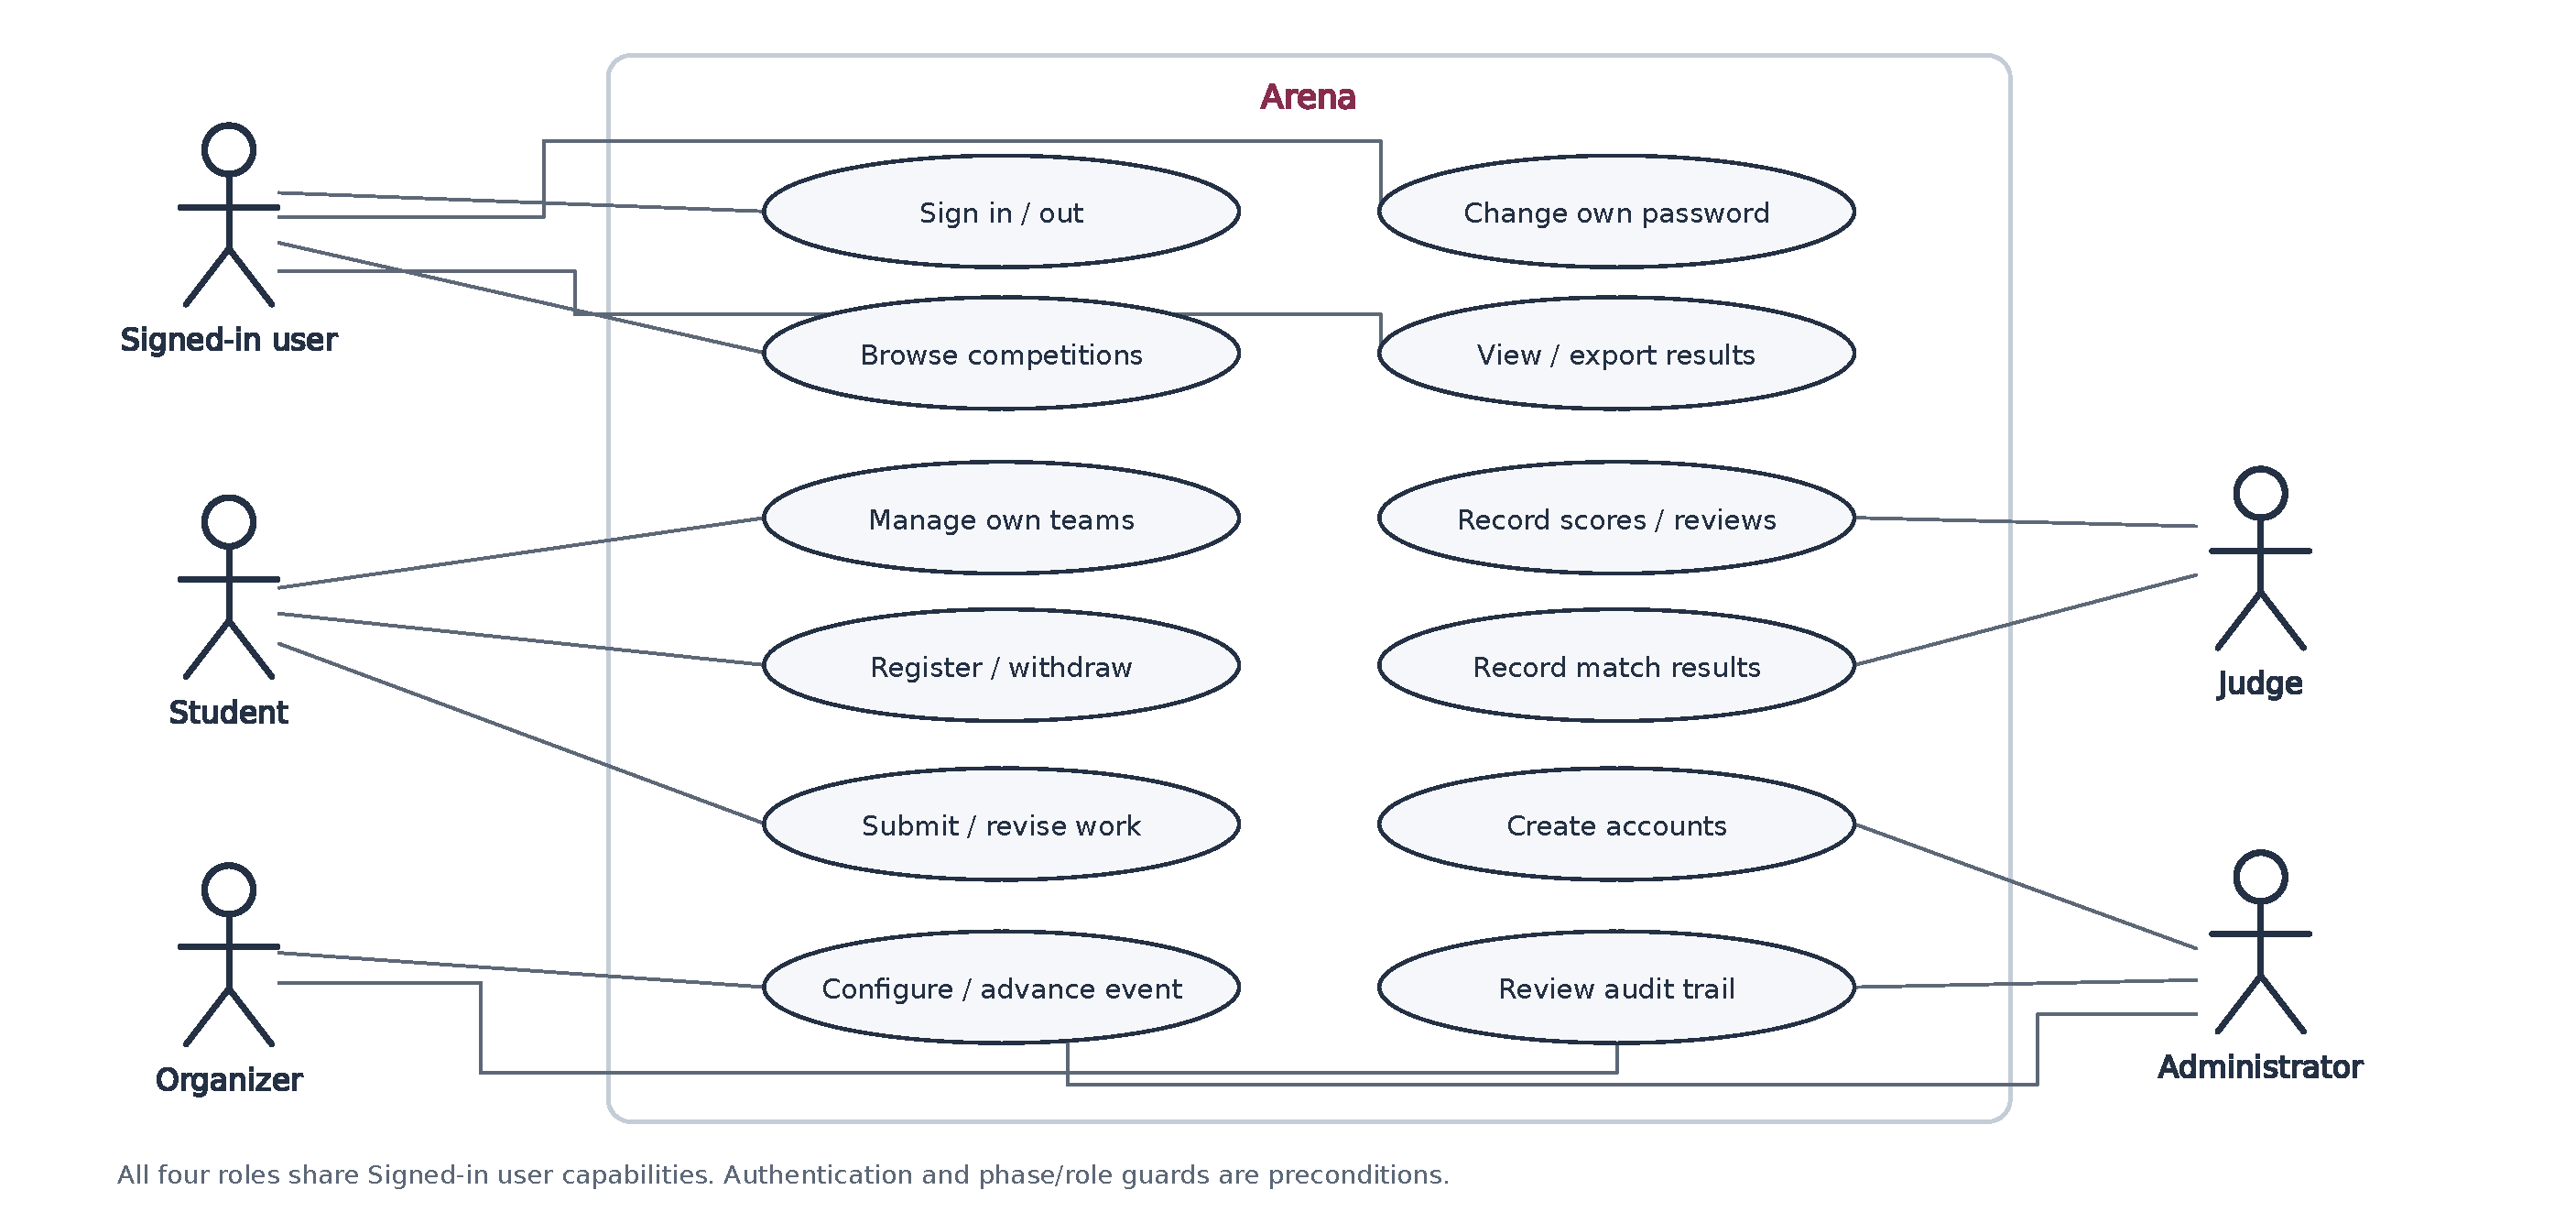
\includegraphics[width=\linewidth,height=11.8cm,keepaspectratio]{../reports/assets/uml/01_use_case.pdf}
\clearpage\subsection*{02 Registration sequence}
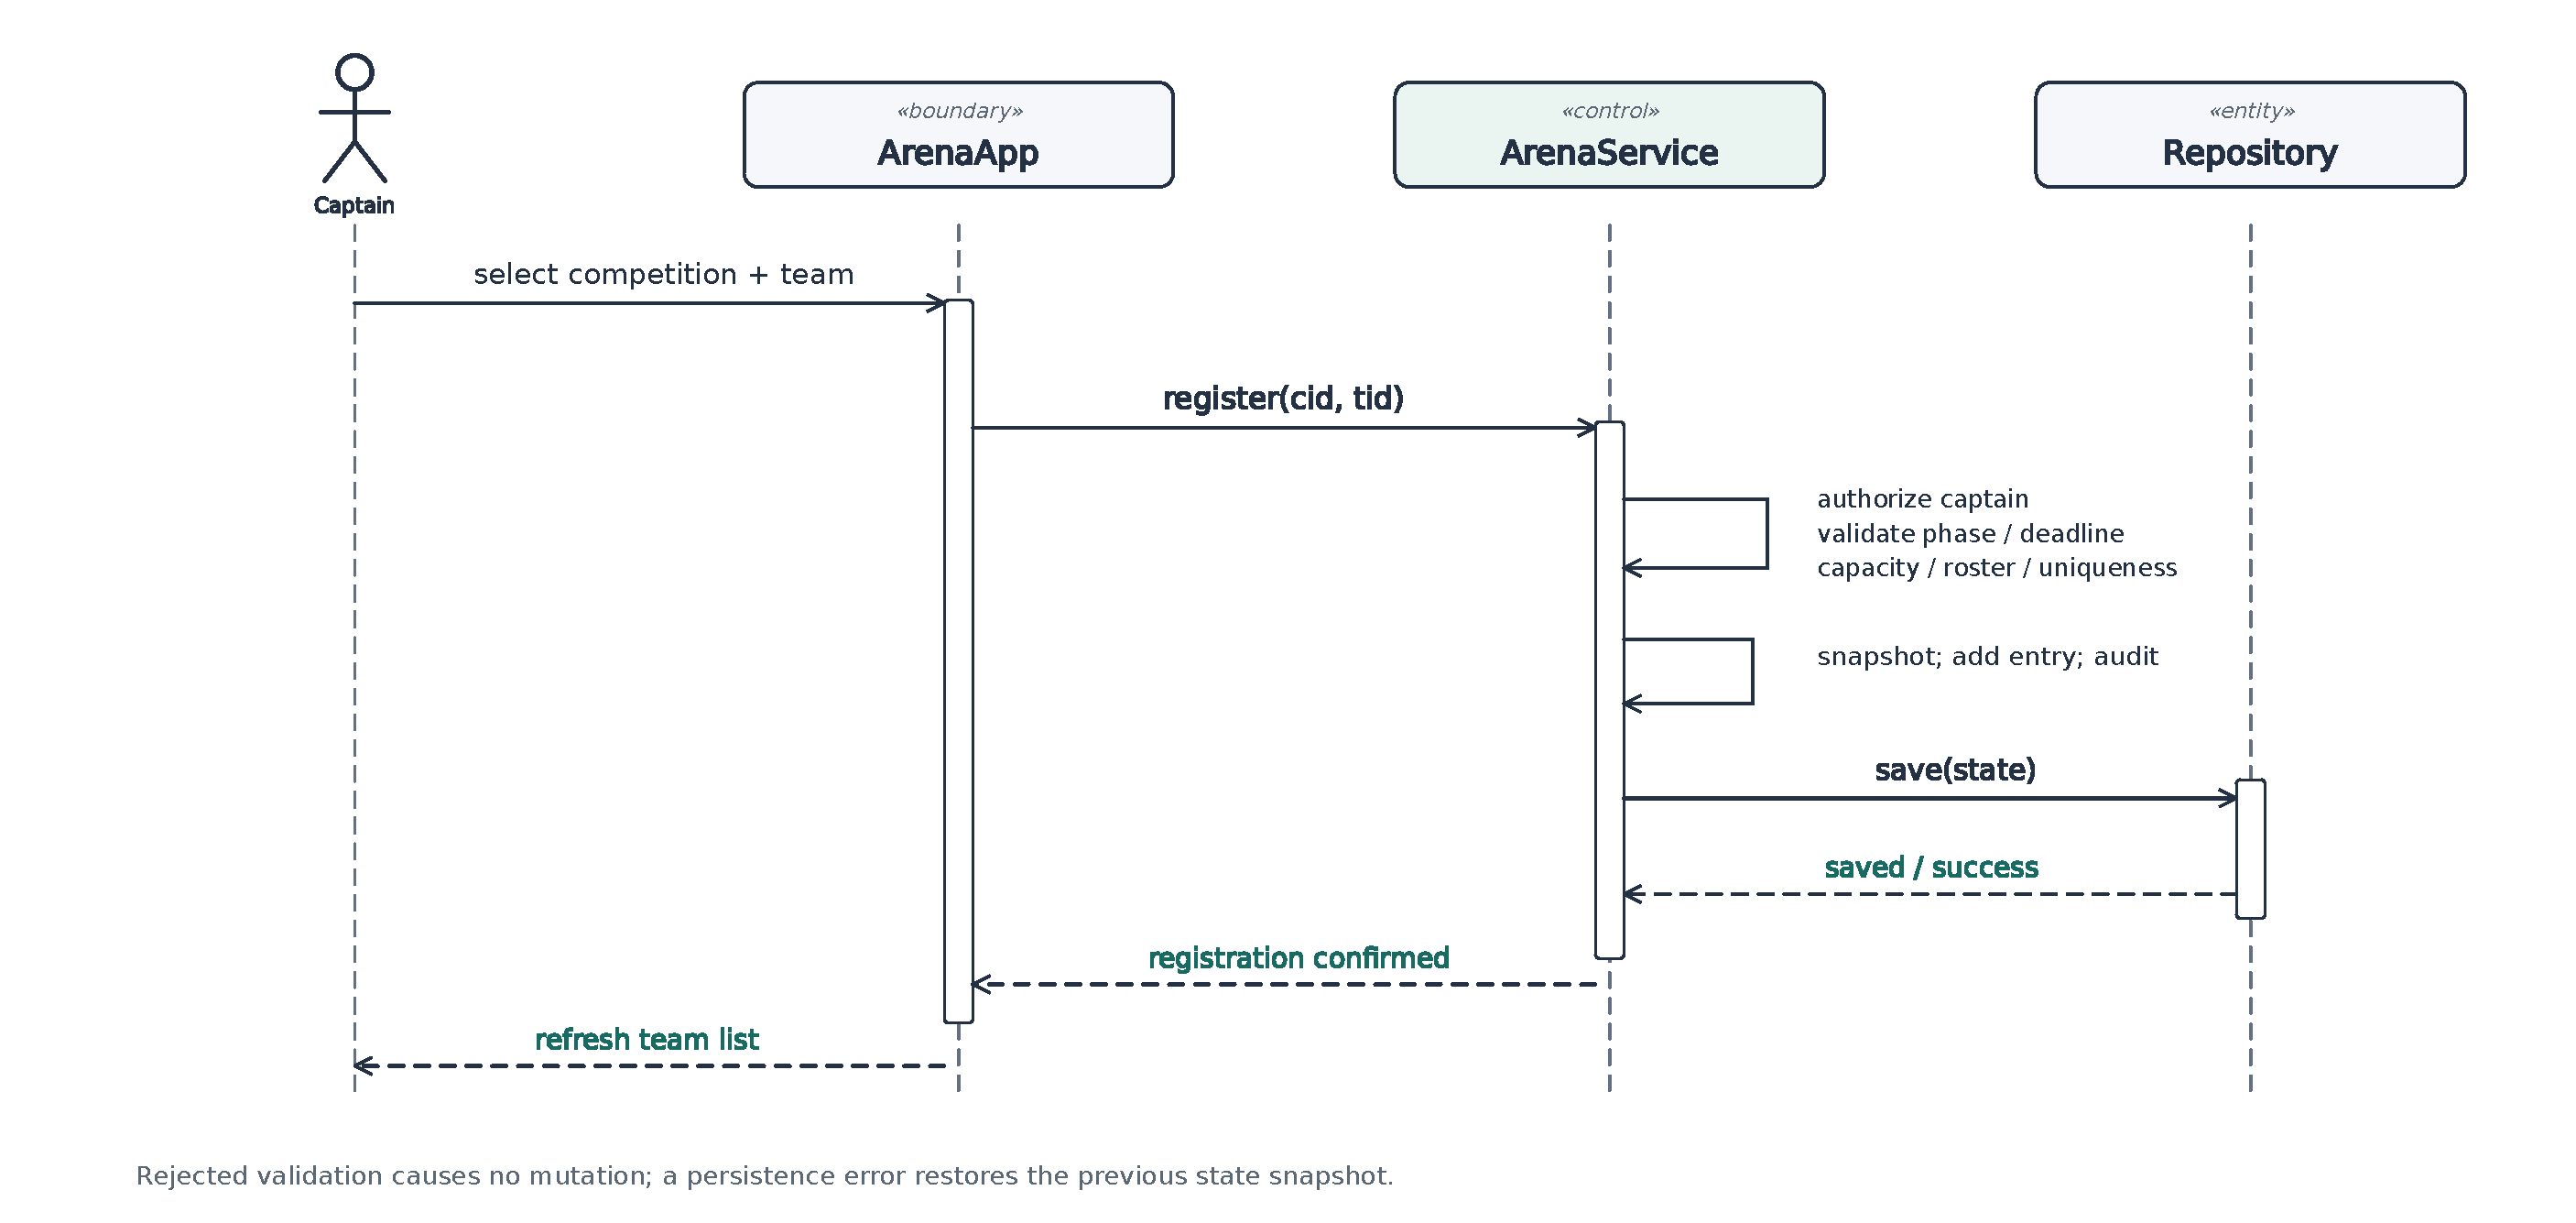
\includegraphics[width=\linewidth,height=13cm,keepaspectratio]{../reports/assets/uml/02_registration_sequence.pdf}
\clearpage\subsection*{03 Competition state machine}
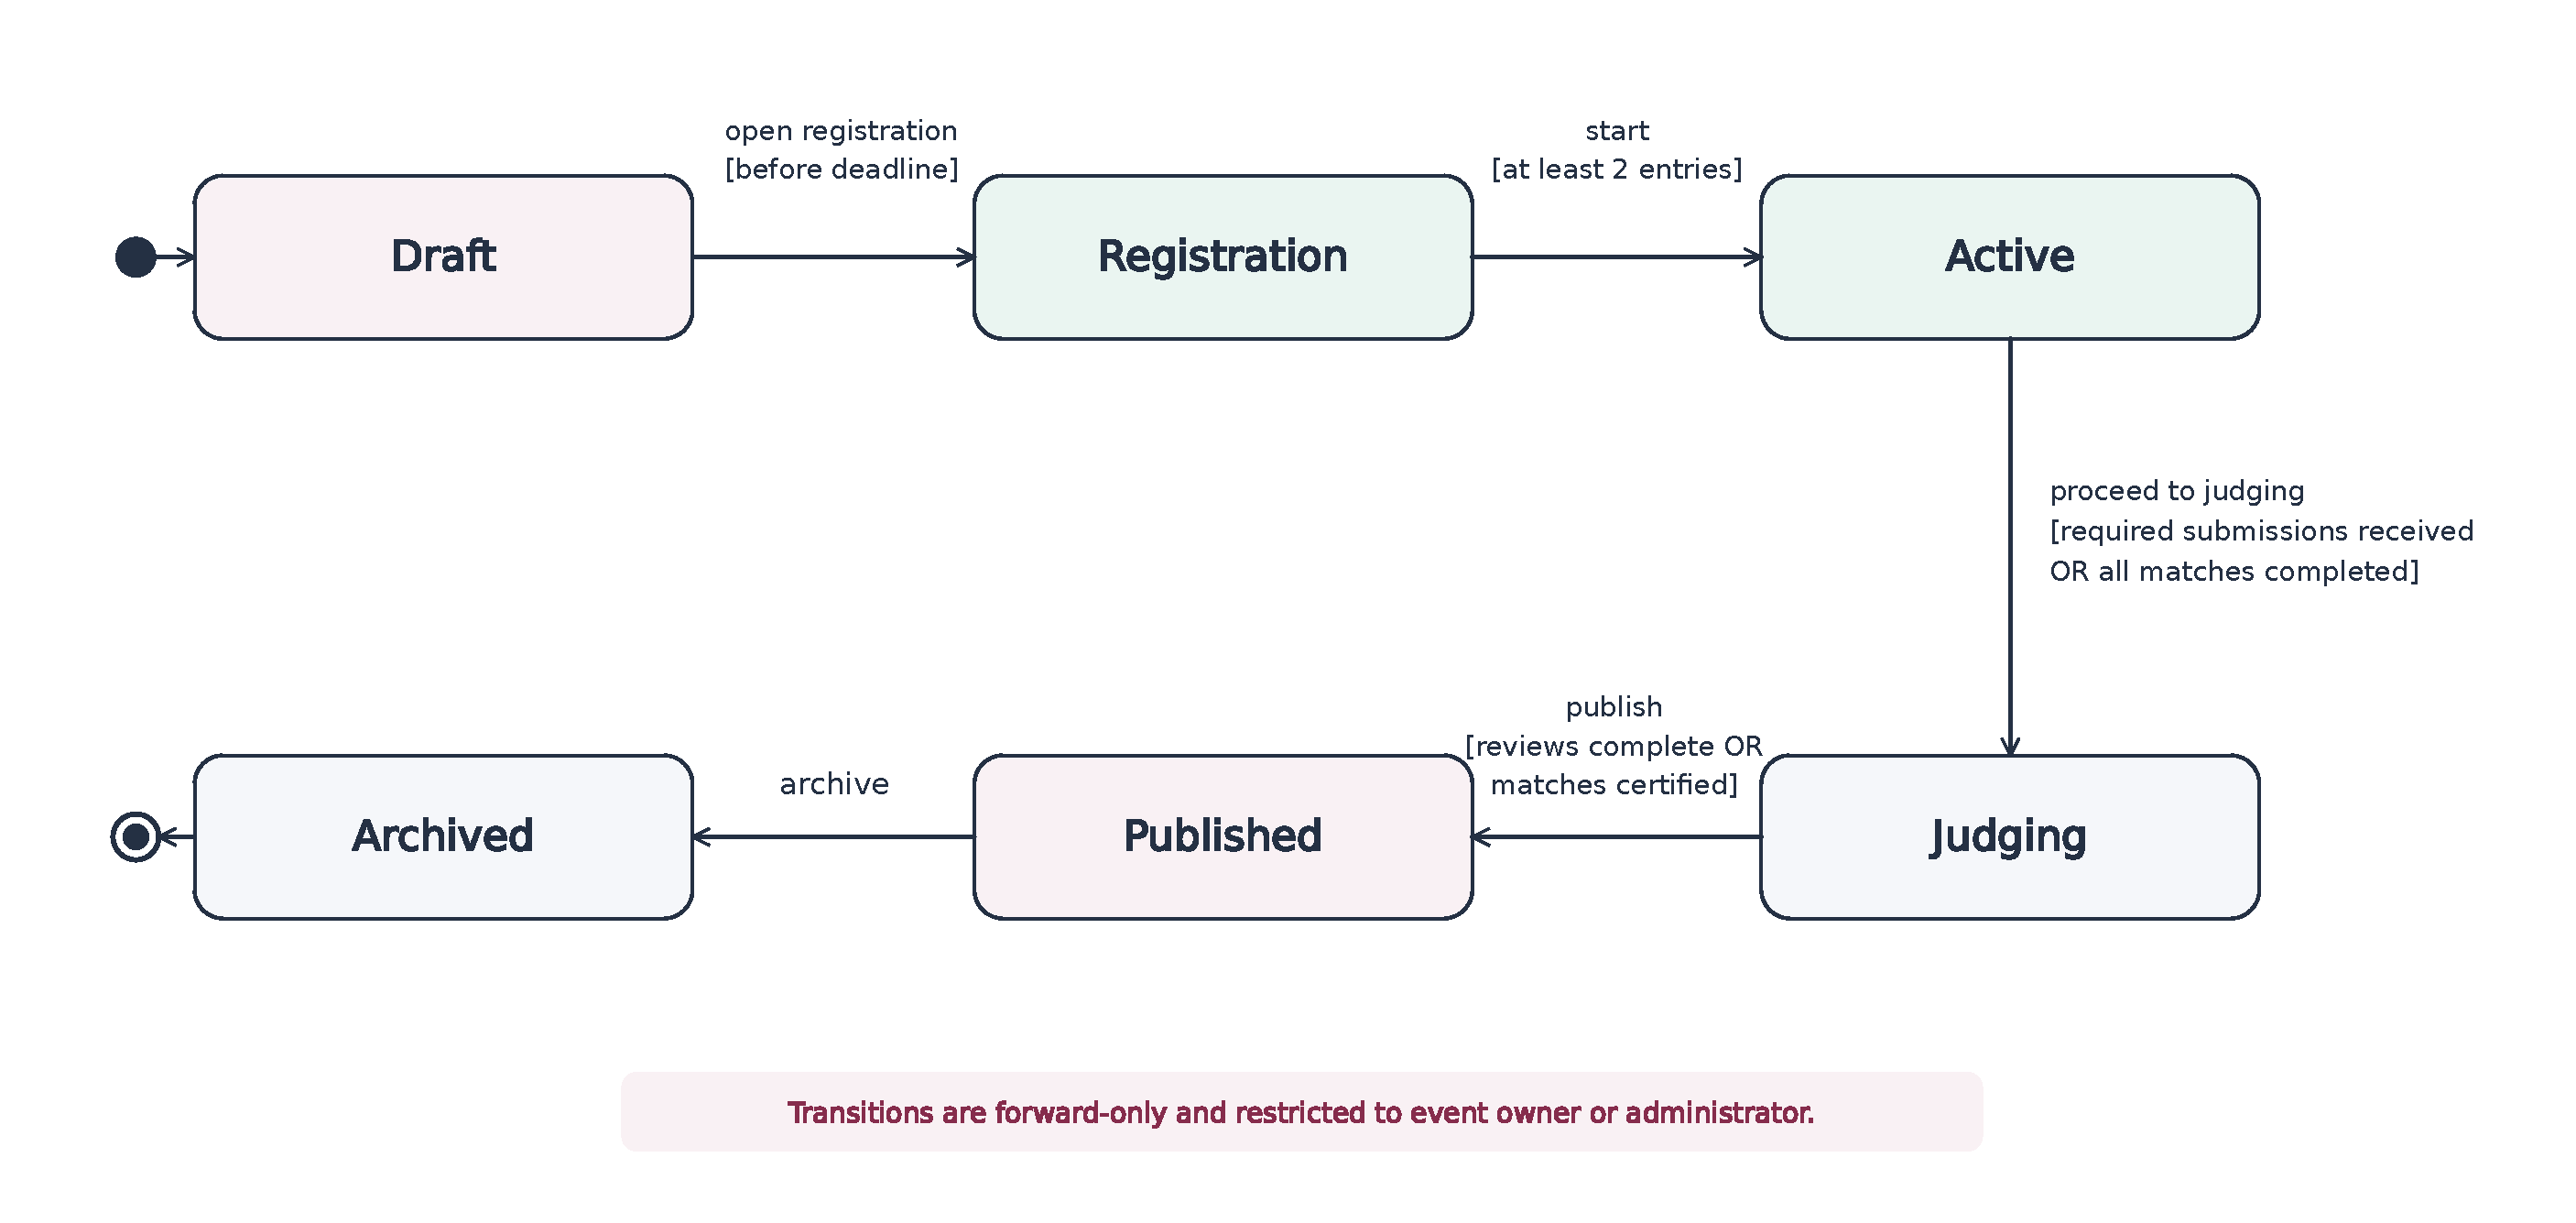
\includegraphics[width=\linewidth,height=13cm,keepaspectratio]{../reports/assets/uml/03_competition_state.pdf}
\clearpage\subsection*{04 Format-specific activity}
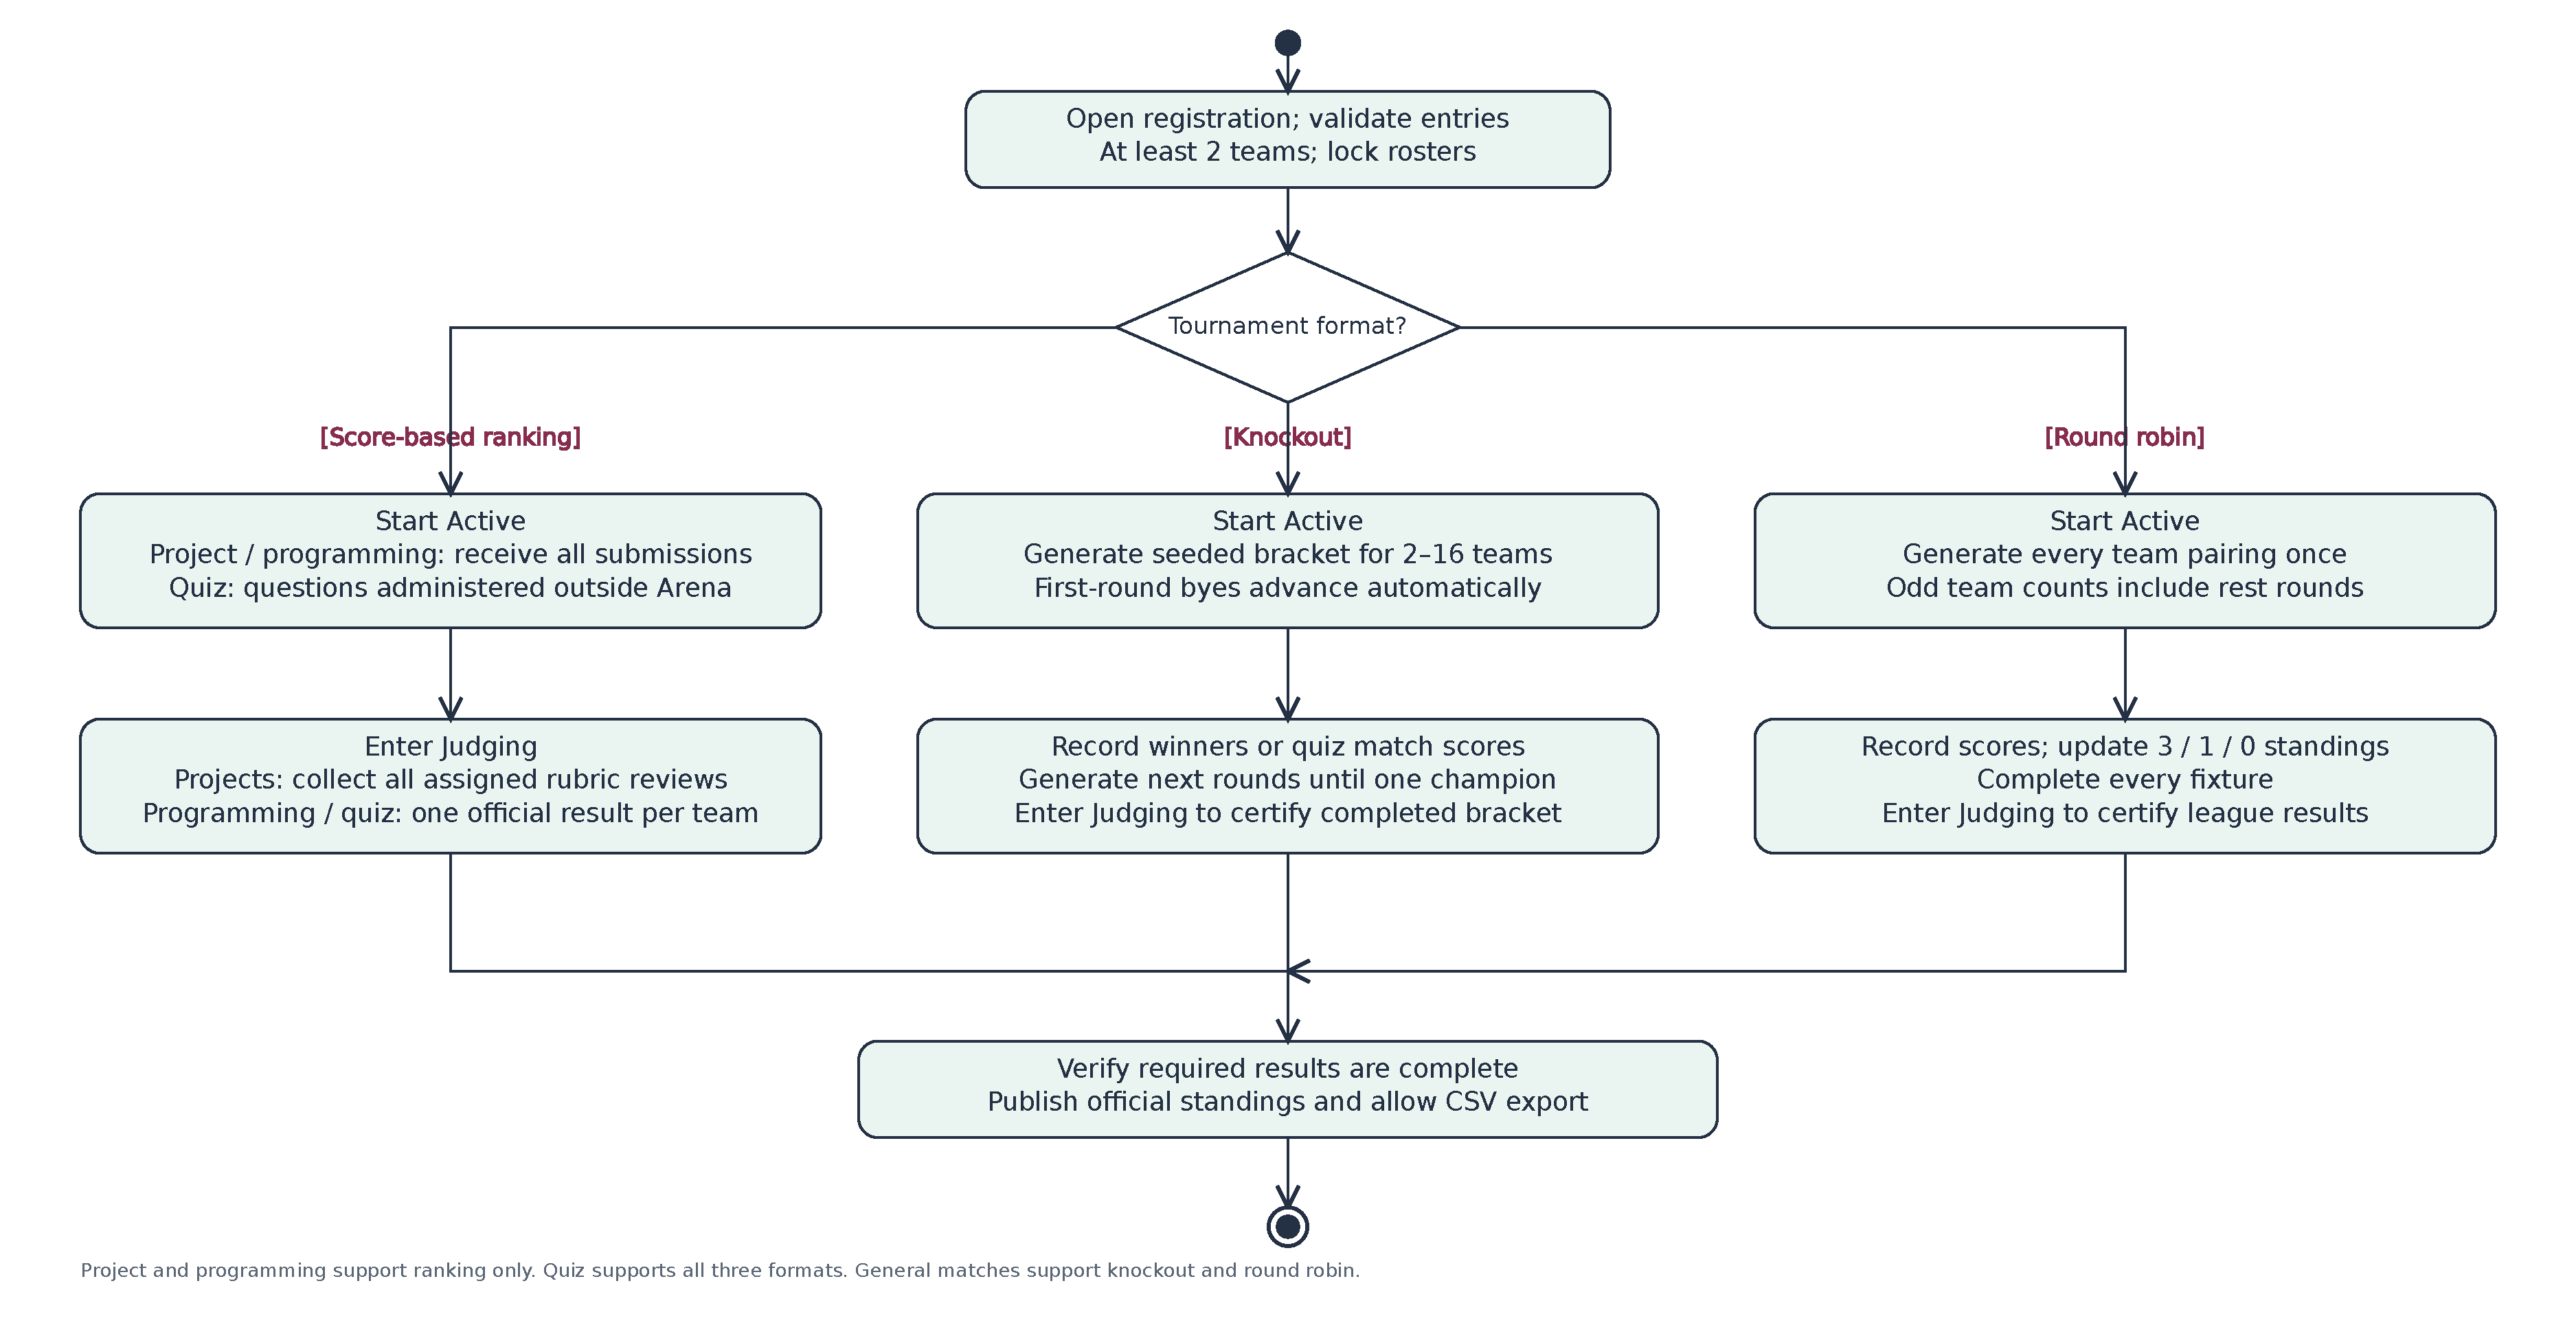
\includegraphics[width=\linewidth,height=13cm,keepaspectratio]{../reports/assets/uml/04_competition_activity.pdf}
\clearpage\subsection*{05 Conceptual domain}
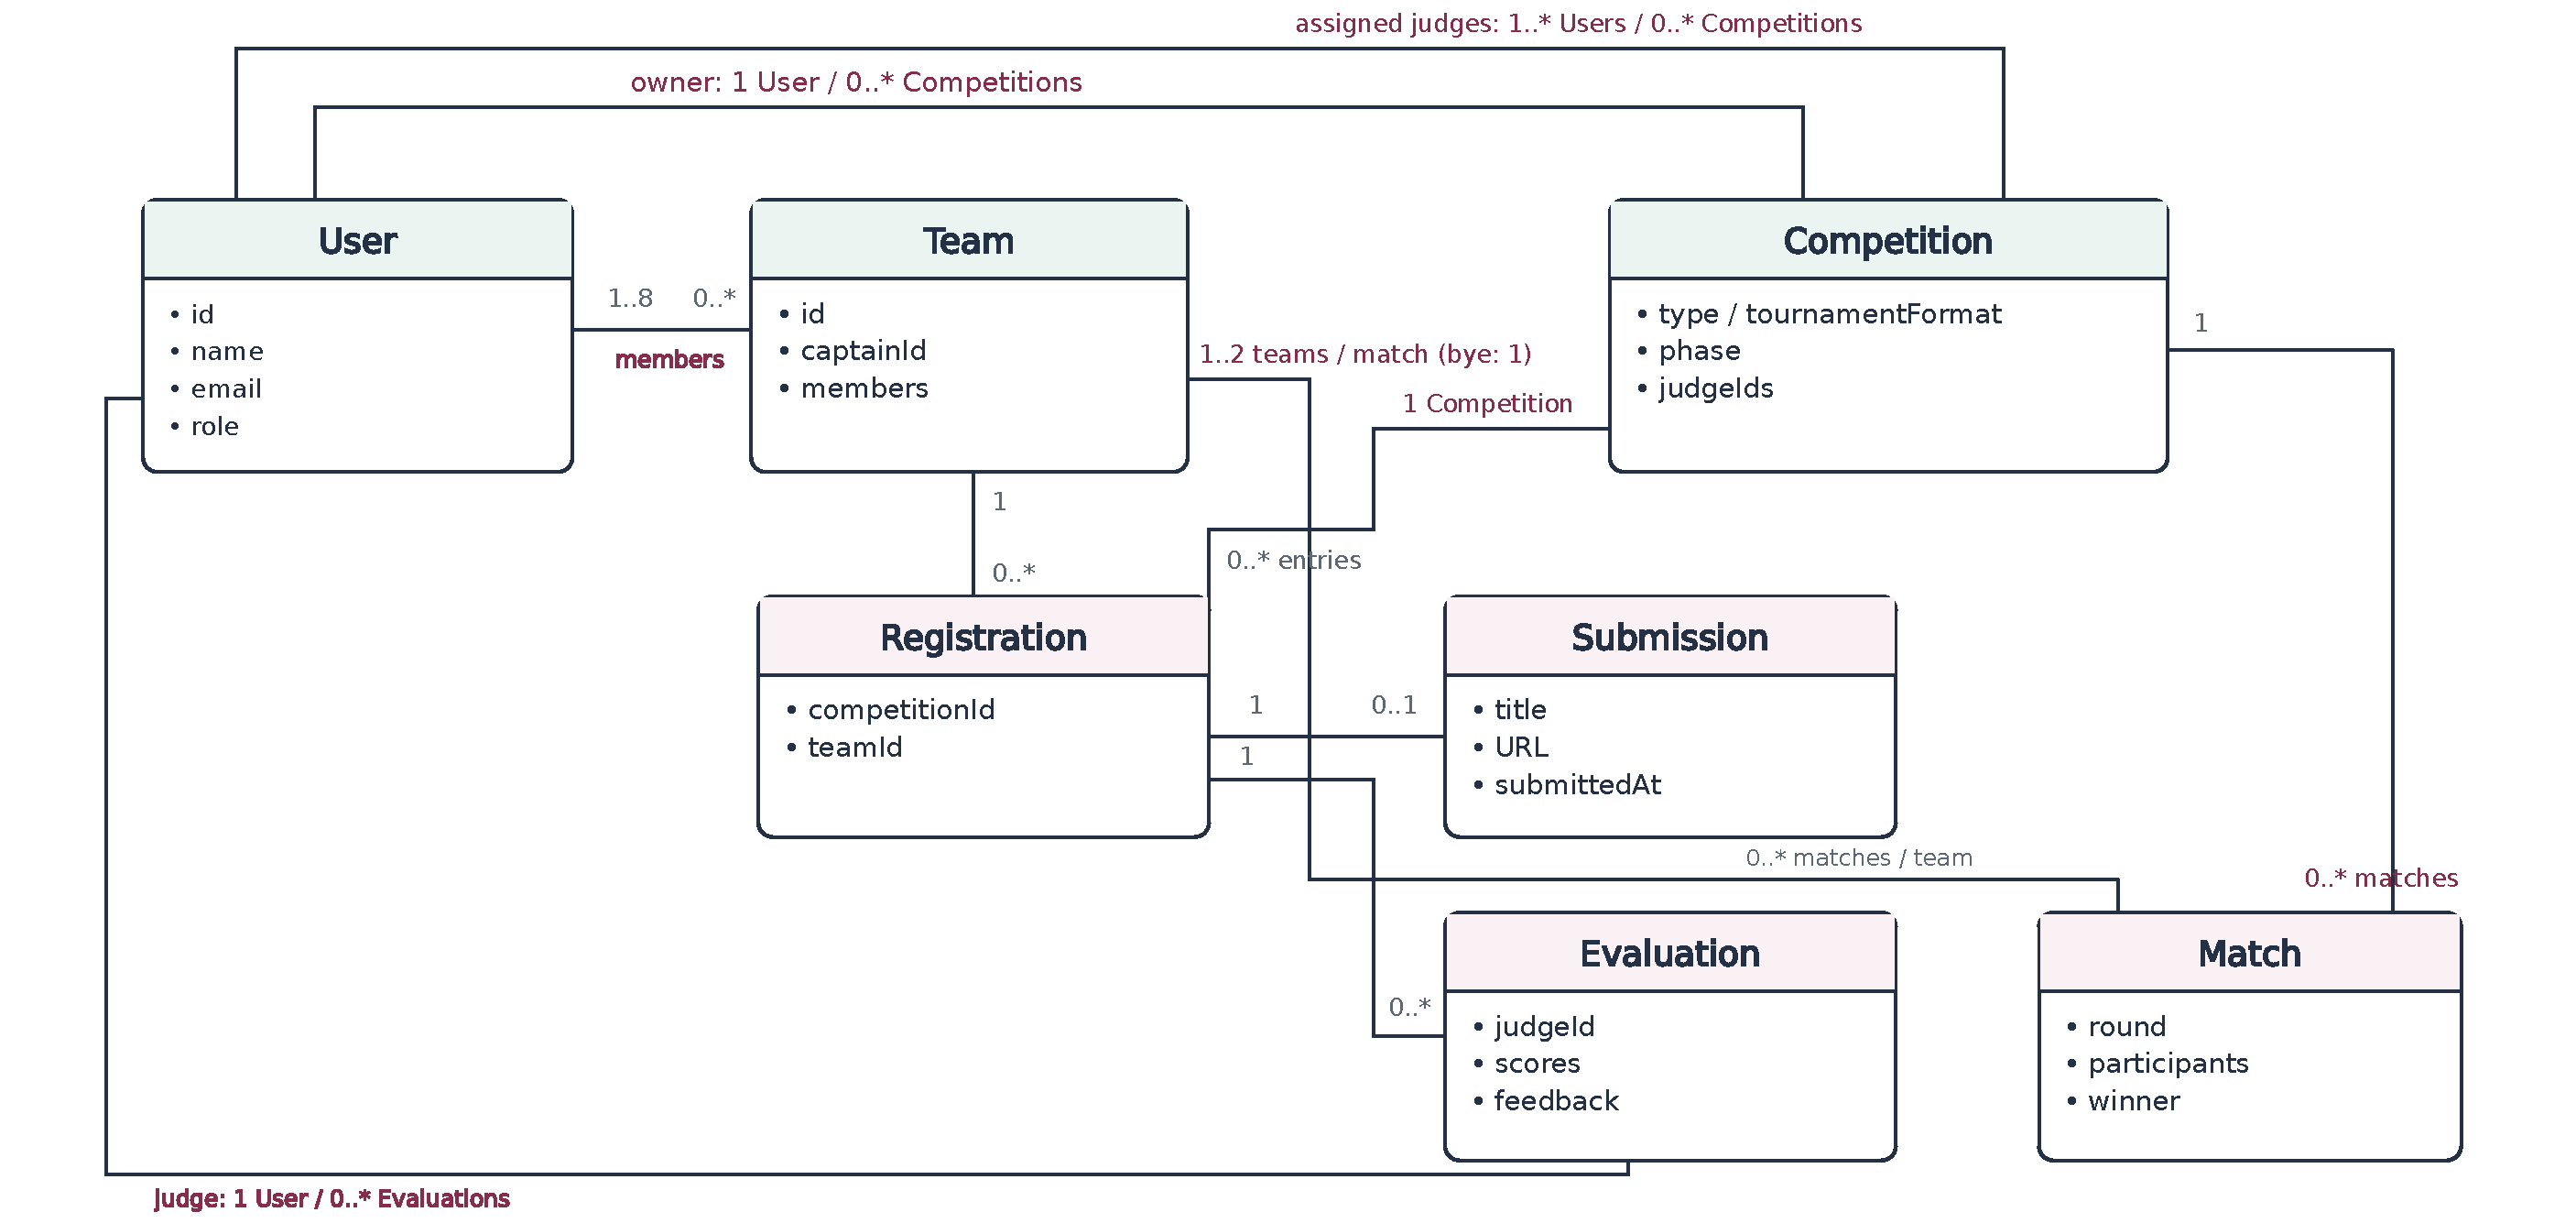
\includegraphics[width=\linewidth,height=13cm,keepaspectratio]{../reports/assets/uml/05_conceptual_domain.pdf}
\clearpage\subsection*{06 Software architecture}
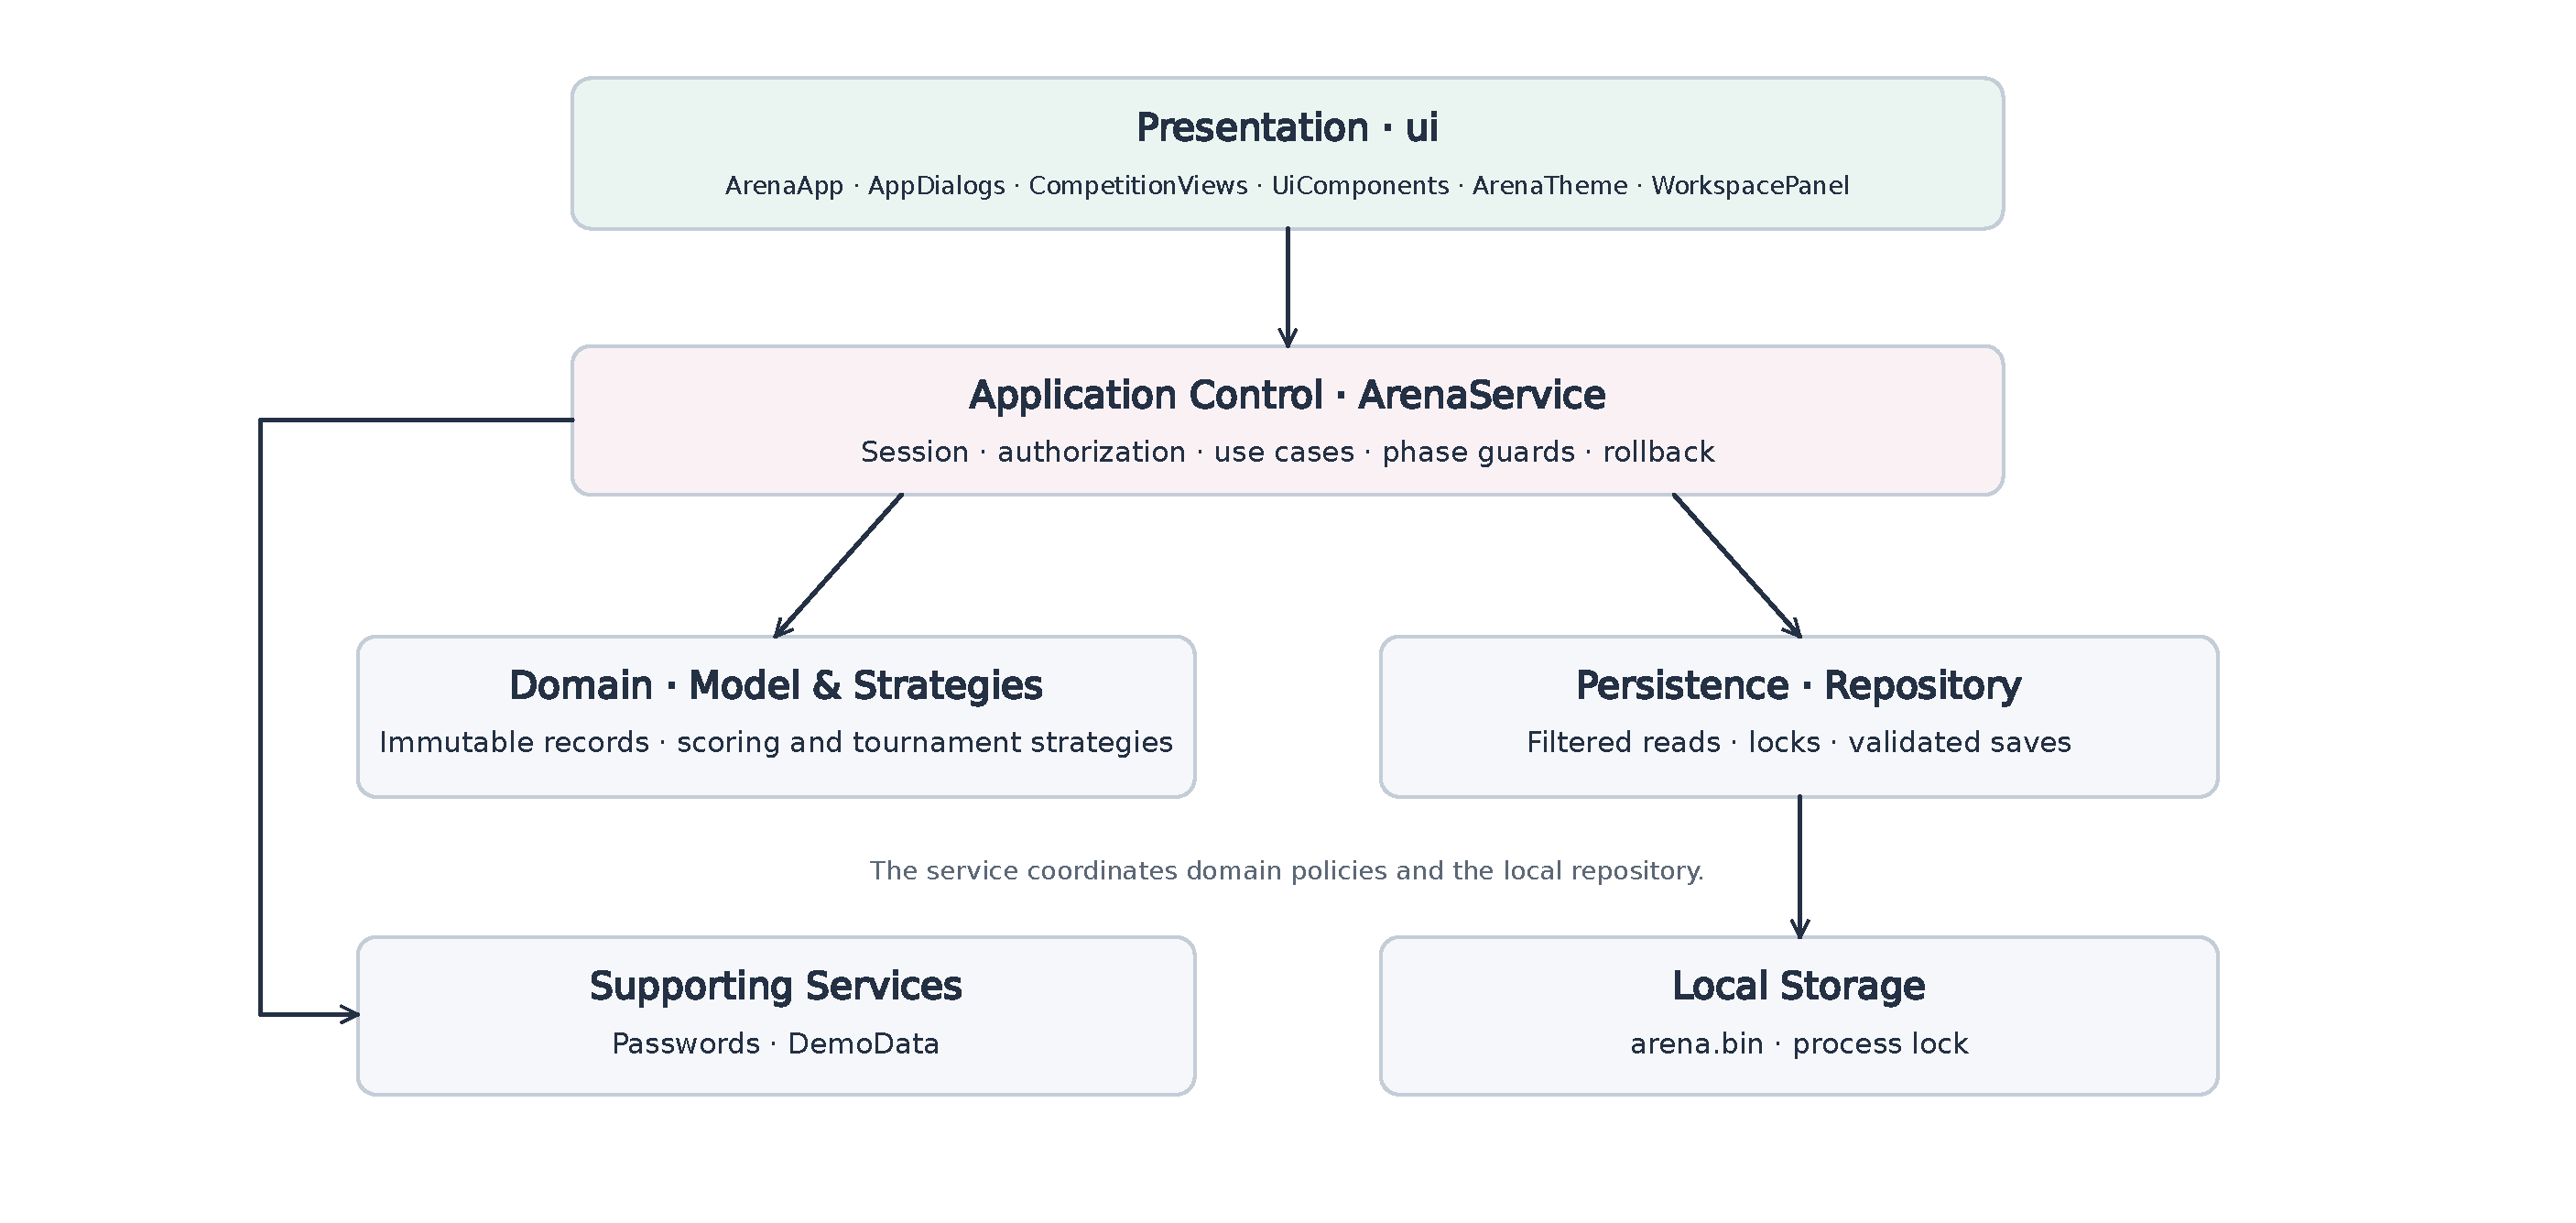
\includegraphics[width=\linewidth,height=13cm,keepaspectratio]{../reports/assets/uml/06_software_architecture.pdf}
\clearpage\subsection*{07 Competition Strategy}
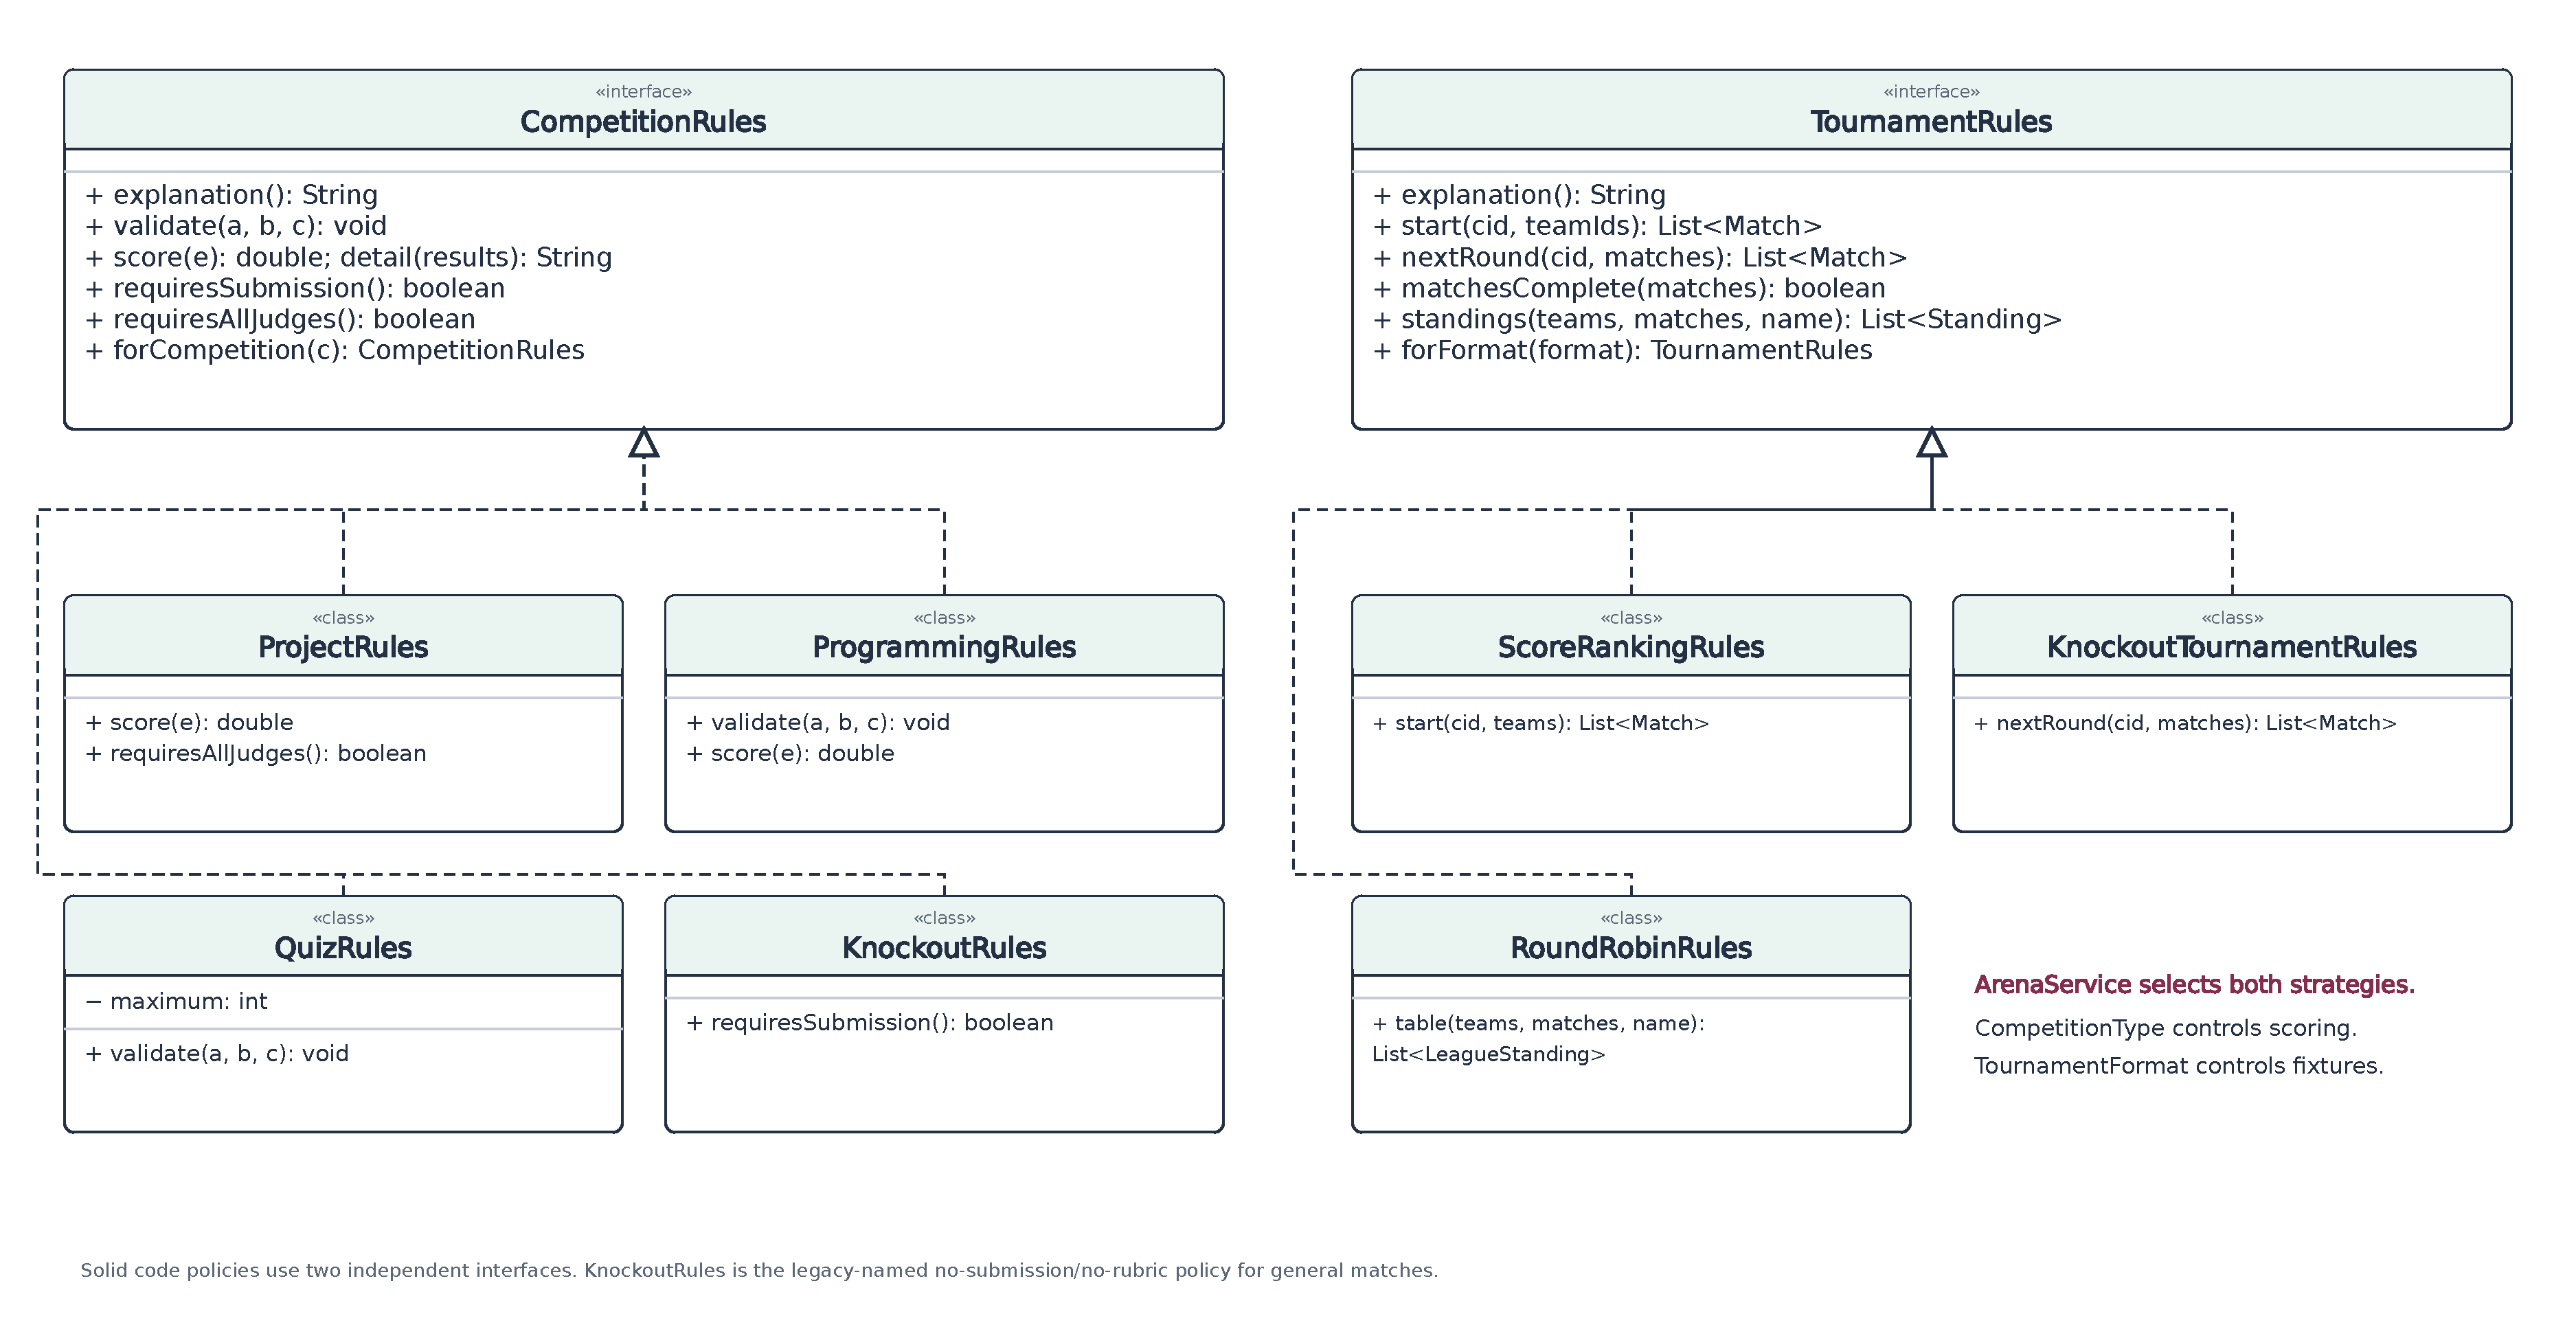
\includegraphics[width=\linewidth,height=13cm,keepaspectratio]{../reports/assets/uml/07_strategy_class.pdf}
\clearpage\subsection*{08 Design Class Diagram}
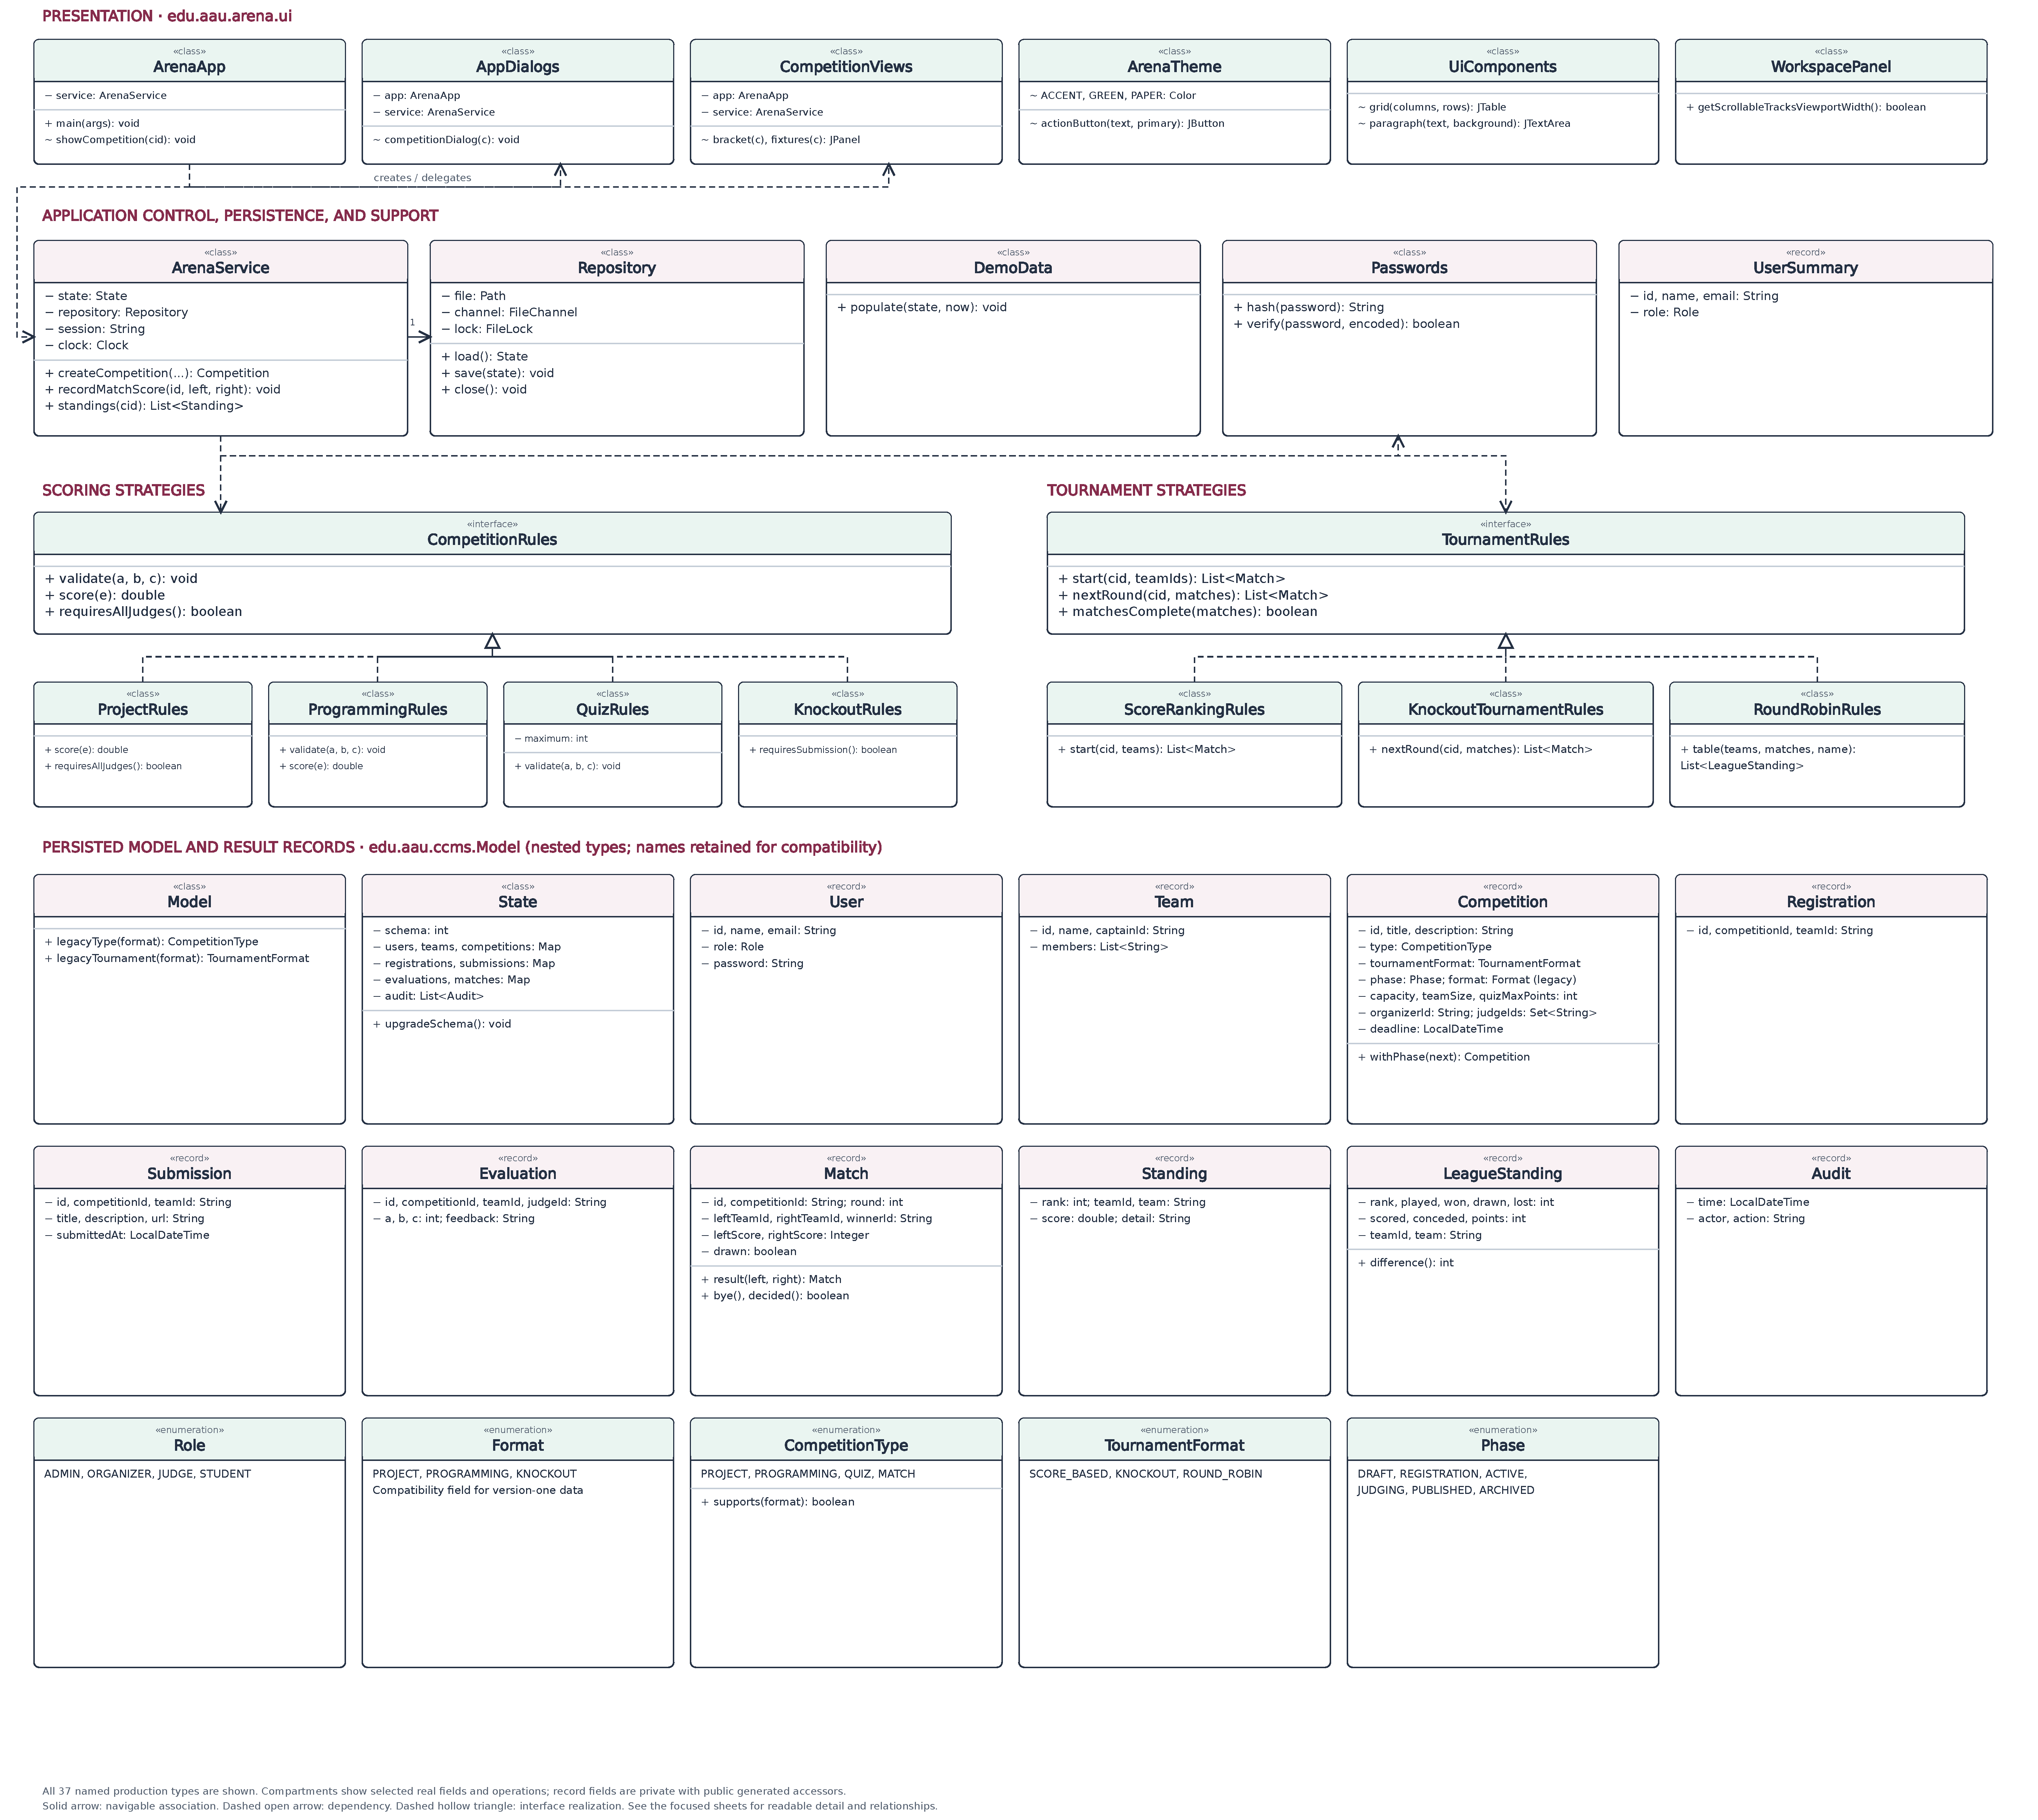
\includegraphics[width=\linewidth,height=13cm,keepaspectratio]{../reports/assets/uml/08_design_class.pdf}
\clearpage\subsection*{08a Application classes}
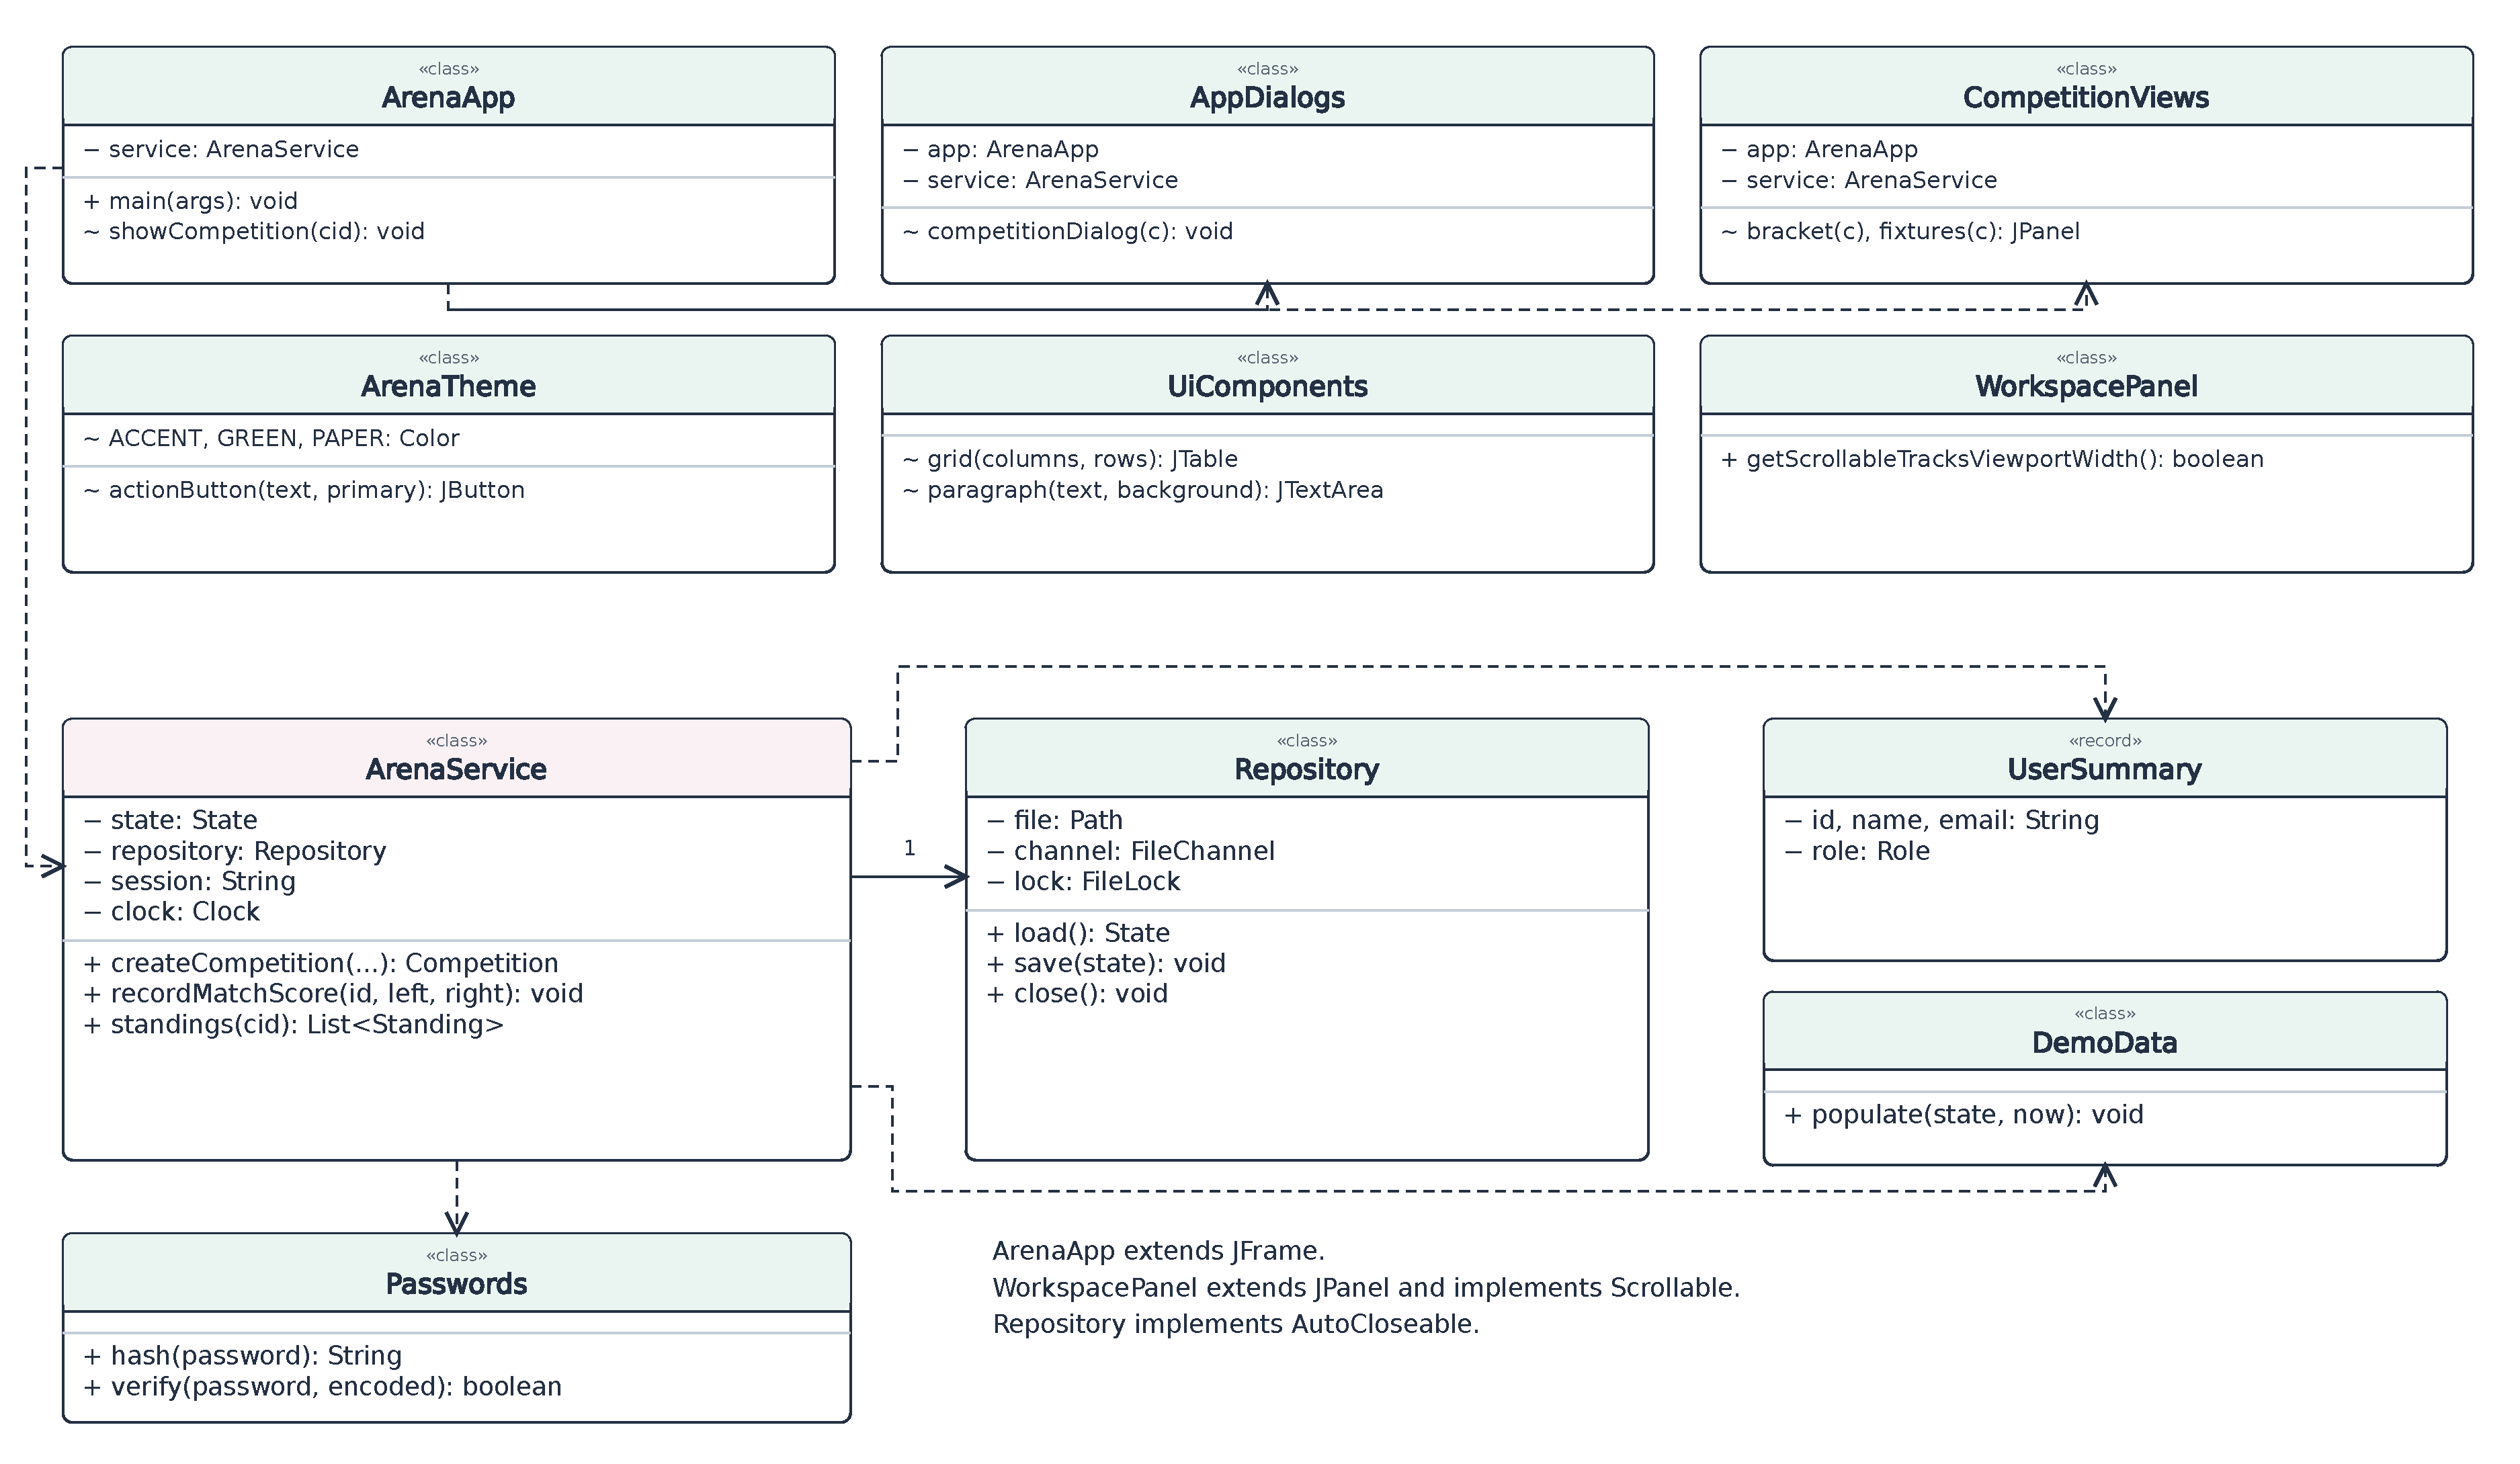
\includegraphics[width=\linewidth,height=13cm,keepaspectratio]{../reports/assets/uml/08a_application_classes.pdf}
\clearpage\subsection*{08b Record classes}
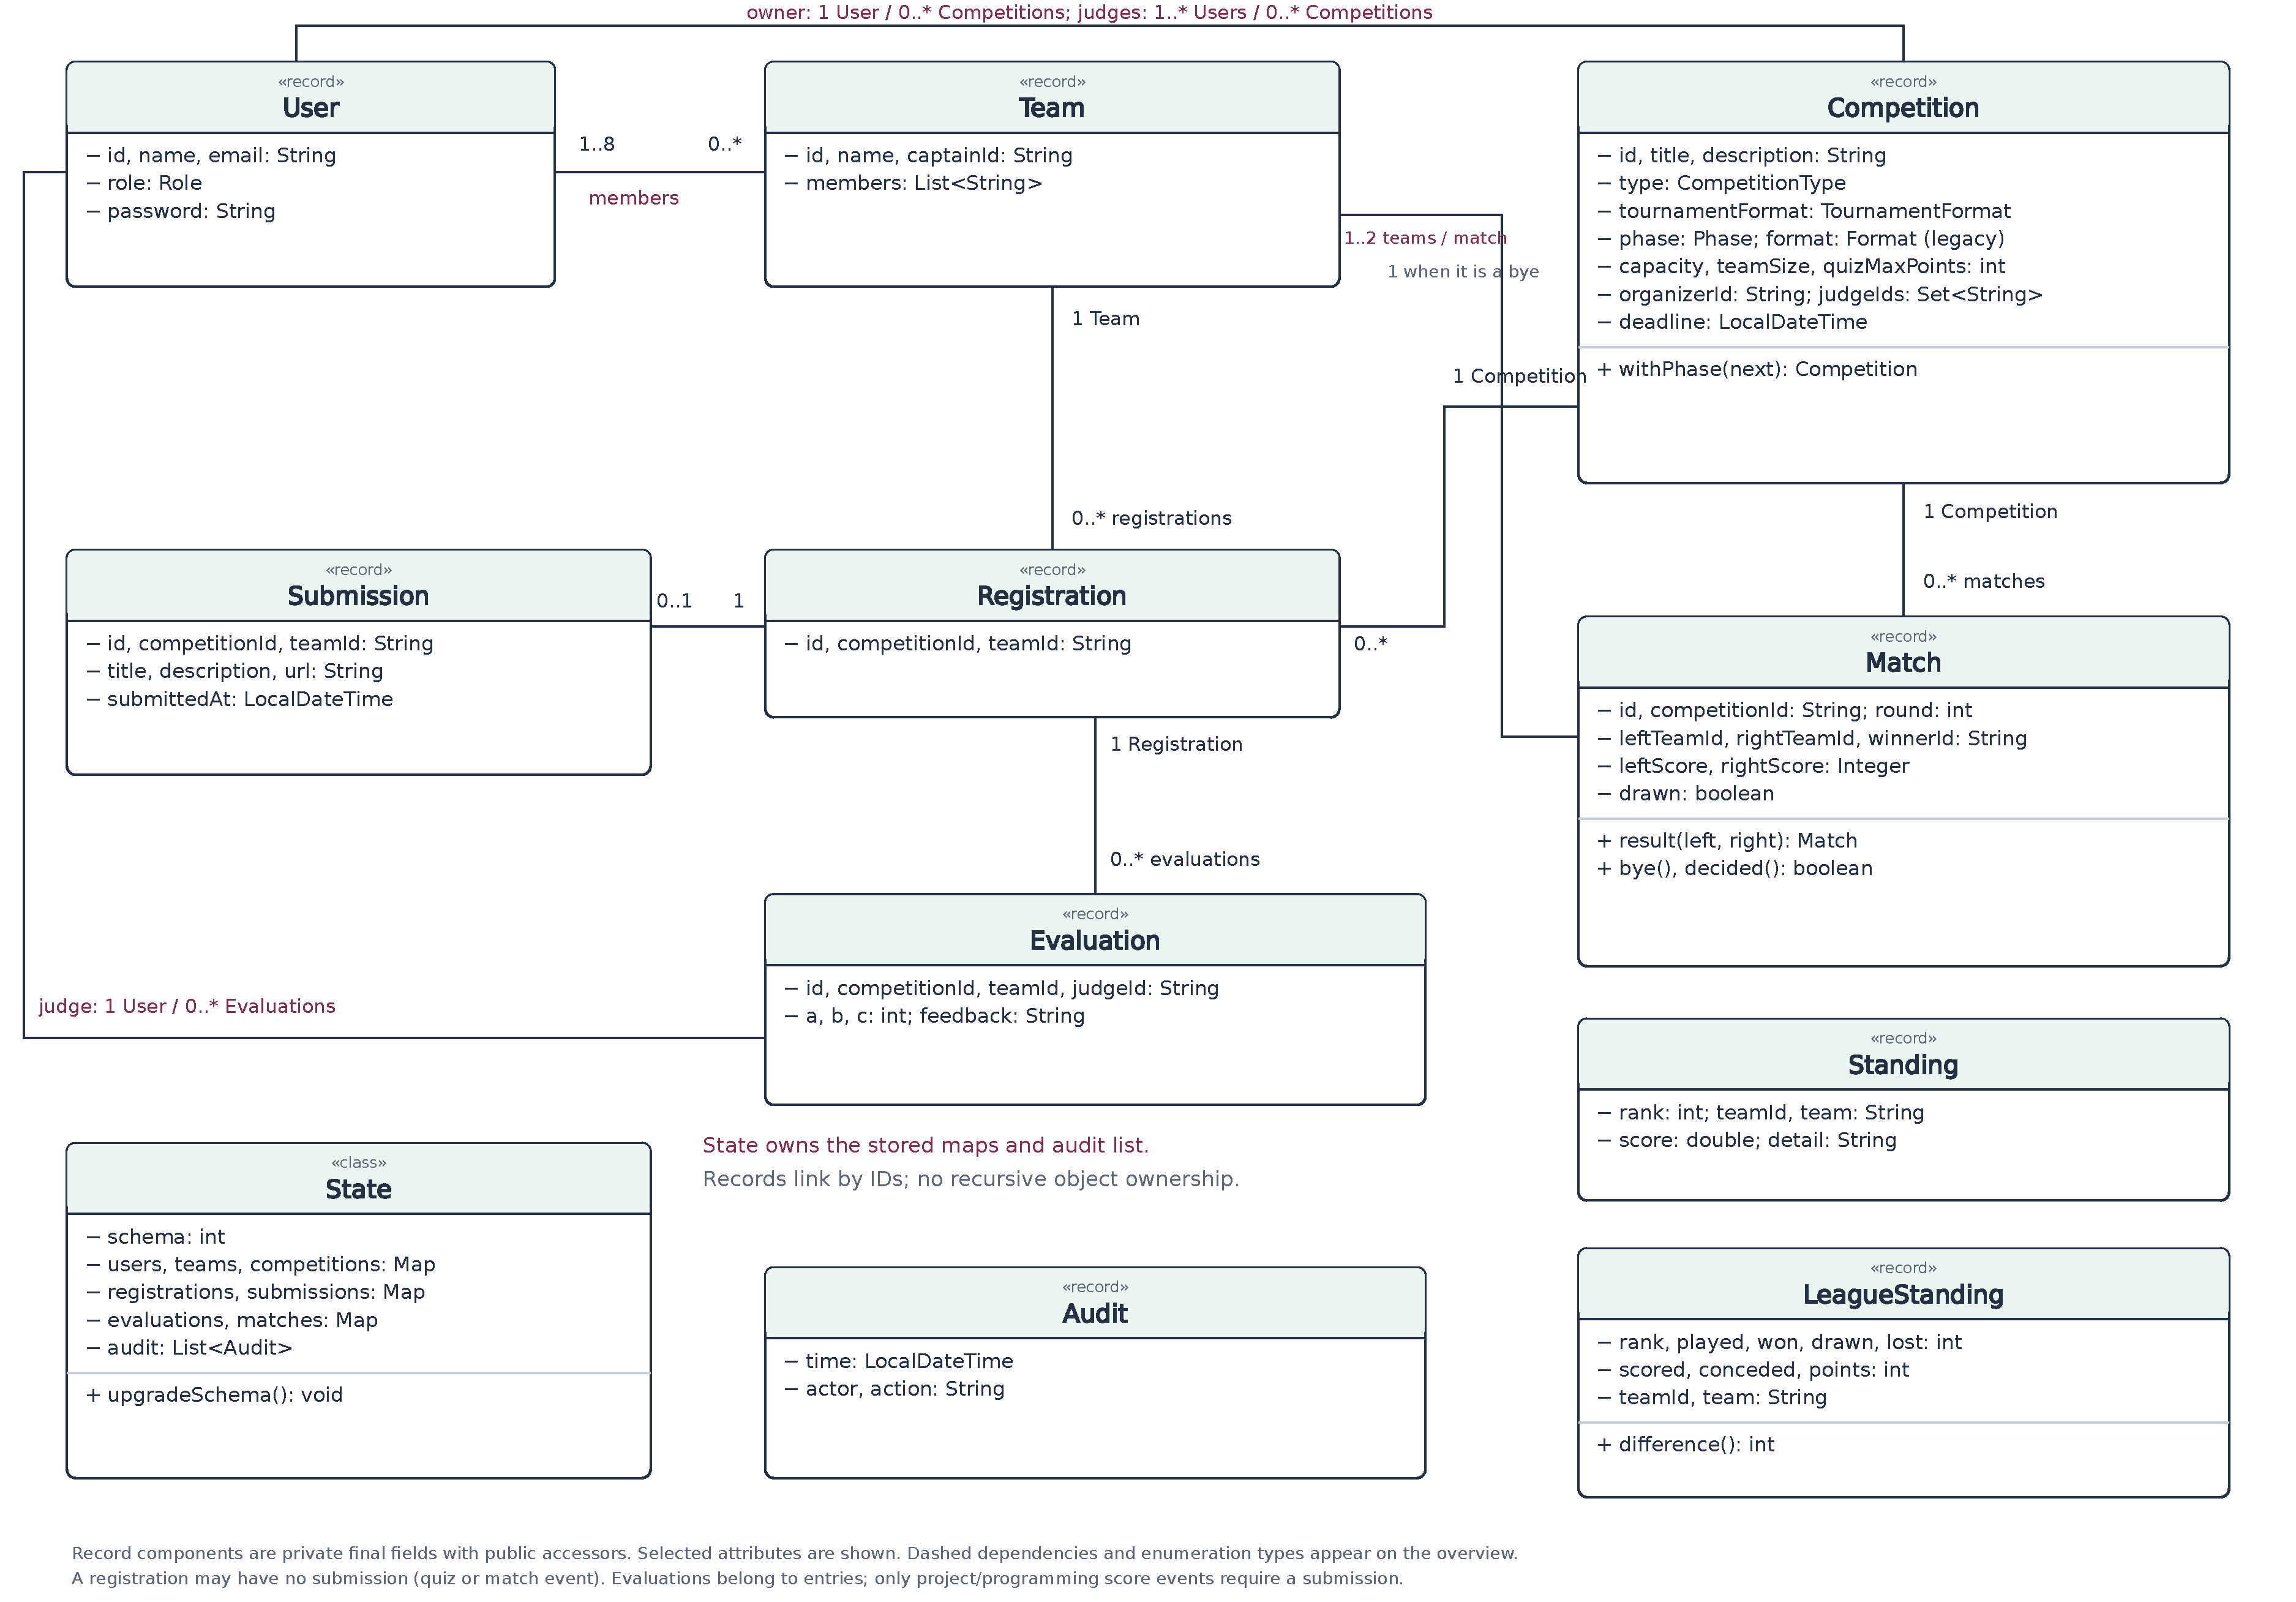
\includegraphics[width=\linewidth,height=13cm,keepaspectratio]{../reports/assets/uml/08b_record_classes.pdf}
\clearpage\subsection*{09 Package dependencies}
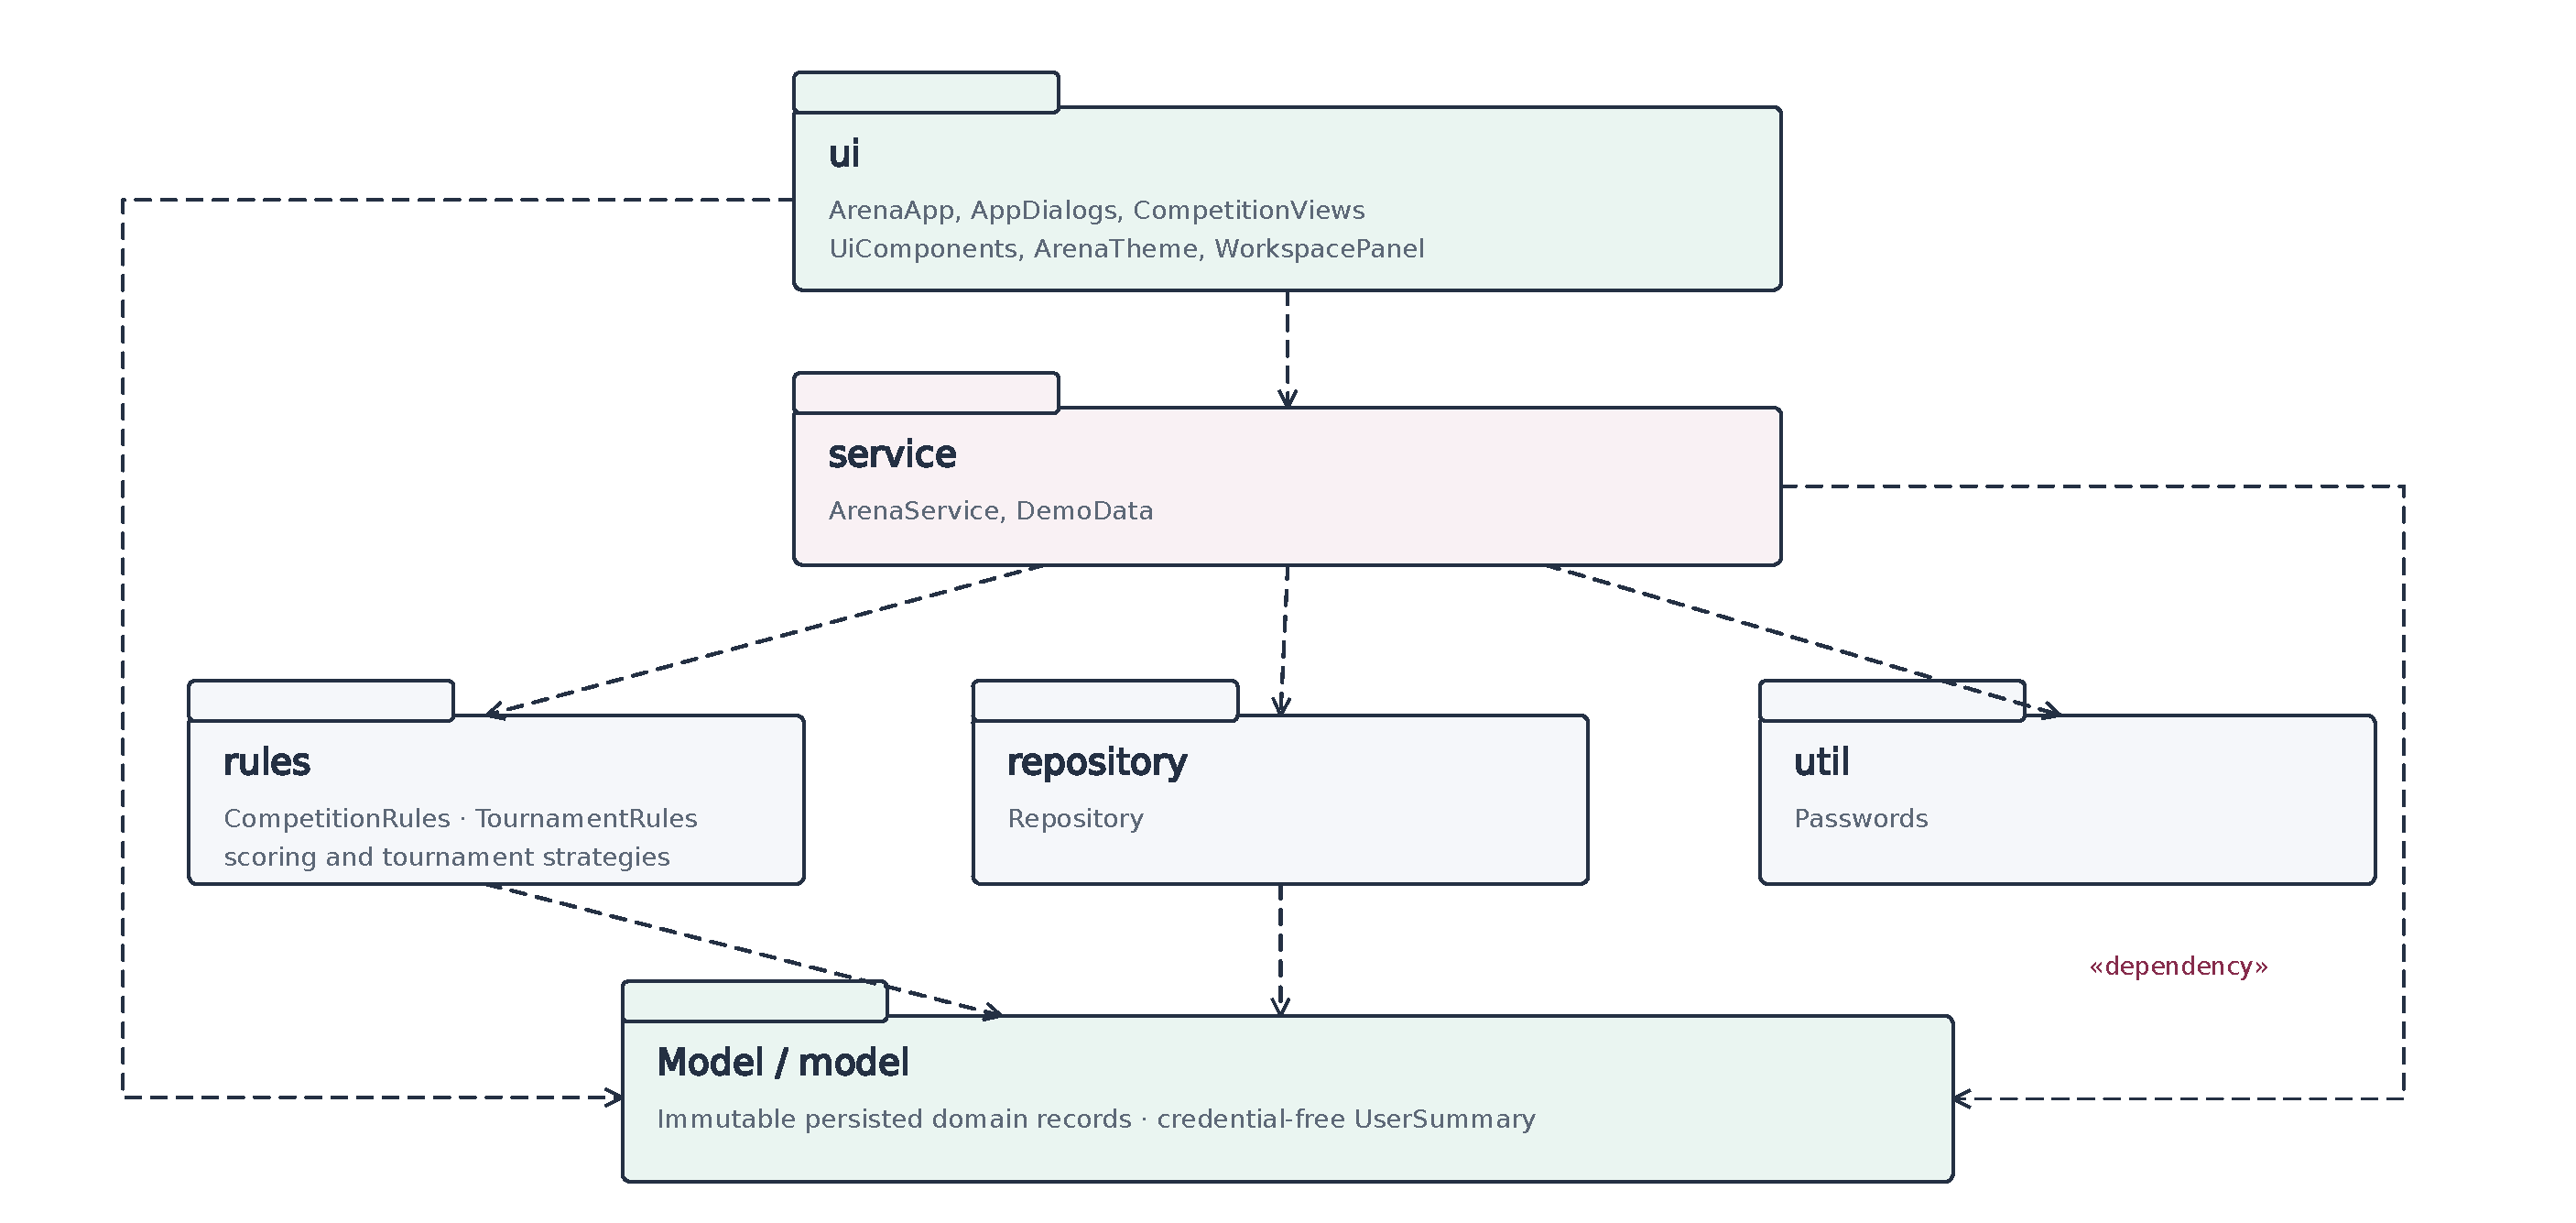
\includegraphics[width=\linewidth,height=13cm,keepaspectratio]{../reports/assets/uml/09_package_dependencies.pdf}
\end{landscape}

\topic{Reading map and source basis}
\begin{itemize}
\item Start with README.md, the professor's supplied approval, and the five original requirements/*.txt outlines.
\item Read reports/source/system-analysis.tex, then reports/source/system-design.tex. Follow the eleven figures in reports/assets/uml.
\item Read Model.java, CompetitionRules and its four implementations, TournamentRules and its three implementations, then ArenaService in the groups explained here.
\item Read Repository and Passwords, followed by DemoData. Trace startup in ArenaApp.main.
\item Read ArenaApp, AppDialogs, CompetitionViews, UiComponents, and ArenaTheme alongside the rendered app screens.
\item Compare prototype/index.html, styles.css, and app.js to the authoritative Java workflows.
\item Read all three custom test runners, AcceptanceMavenTest, and reports/test-evidence. Use the Testing Report for requirements mapping.
\item Read the Implementation Report/User Guide, Interface Mock-ups, the technical review and demo-data notes in project-notes, build scripts, pom.xml, packaging helper, and presentation/speaking-script-and-demo.md.
\end{itemize}
This guide describes the updated Arena implementation and the actual 10 November 2026 verification. The original pre-Arena guide remains in the private local archive. The persisted compatibility namespace and old-data fixtures are retained intentionally. Individual development contributions are not inferred from these explanations or speaking assignments.
\end{document}
